\documentclass{book}
\usepackage[a4paper,top=2.5cm,bottom=2.5cm,left=2.5cm,right=2.5cm]{geometry}
\usepackage{makeidx}
\usepackage{natbib}
\usepackage{graphicx}
\usepackage{multicol}
\usepackage{float}
\usepackage{listings}
\usepackage{color}
\usepackage{ifthen}
\usepackage[table]{xcolor}
\usepackage{textcomp}
\usepackage{alltt}
\usepackage{ifpdf}
\ifpdf
\usepackage[pdftex,
            pagebackref=true,
            colorlinks=true,
            linkcolor=blue,
            unicode
           ]{hyperref}
\else
\usepackage[ps2pdf,
            pagebackref=true,
            colorlinks=true,
            linkcolor=blue,
            unicode
           ]{hyperref}
\usepackage{pspicture}
\fi
\usepackage[utf8]{inputenc}
\usepackage{hfont}

\usepackage{mathptmx}
\usepackage[scaled=.90]{helvet}
\usepackage{courier}
\usepackage{sectsty}
\usepackage{amssymb}
\usepackage[titles]{tocloft}
\usepackage{doxygen}
\lstset{language=C++,inputencoding=utf8,basicstyle=\footnotesize,breaklines=true,breakatwhitespace=true,tabsize=4,numbers=left }
\makeindex
\setcounter{tocdepth}{3}
\renewcommand{\footrulewidth}{0.4pt}
\renewcommand{\familydefault}{\sfdefault}
\hfuzz=15pt
\setlength{\emergencystretch}{15pt}
\hbadness=750
\tolerance=750
\begin{document}
\hypersetup{pageanchor=false,citecolor=blue}
\begin{titlepage}
\vspace*{7cm}
\begin{center}
{\Large My\-Image\-Processing \\[1ex]\large 1.\-0.\-0 }\\
\vspace*{1cm}
{\large 다음에 의해 생성됨 \-:  Doxygen 1.8.2}\\
\vspace*{0.5cm}
{\small 월 11월 19 2012 19:28:15}\\
\end{center}
\end{titlepage}
\clearemptydoublepage
\pagenumbering{roman}
\tableofcontents
\clearemptydoublepage
\pagenumbering{arabic}
\hypersetup{pageanchor=true,citecolor=blue}
\chapter{My\-Image}
\label{index}\hypertarget{index}{}\input{index}
\chapter{계통도 색인}
\section{클래스 계통도}
이 상속 목록은 완전하진 않지만 알파벳순으로 대략적으로 정렬되어있습니다.\-:\begin{DoxyCompactList}
\item \contentsline{section}{\-\_\-\-P\-O\-I\-N\-T}{\pageref{class___p_o_i_n_t}}{}
\item C\-Dialog\begin{DoxyCompactList}
\item \contentsline{section}{C\-Binth\-Set}{\pageref{class_c_binth_set}}{}
\item \contentsline{section}{C\-Pow\-Dlg}{\pageref{class_c_pow_dlg}}{}
\item \contentsline{section}{C\-Scl\-Dlg}{\pageref{class_c_scl_dlg}}{}
\end{DoxyCompactList}
\item C\-Dialog\-Ex\begin{DoxyCompactList}
\item \contentsline{section}{C\-About\-Dlg}{\pageref{class_c_about_dlg}}{}
\item \contentsline{section}{C\-H\-B\-Dlg}{\pageref{class_c_h_b_dlg}}{}
\item \contentsline{section}{C\-Hist\-Dlg}{\pageref{class_c_hist_dlg}}{}
\end{DoxyCompactList}
\item C\-Document\begin{DoxyCompactList}
\item \contentsline{section}{C\-My\-Image\-Processing\-Doc}{\pageref{class_c_my_image_processing_doc}}{}
\end{DoxyCompactList}
\item C\-M\-D\-I\-Child\-Wnd\begin{DoxyCompactList}
\item \contentsline{section}{C\-Child\-Frame}{\pageref{class_c_child_frame}}{}
\end{DoxyCompactList}
\item C\-M\-D\-I\-Frame\-Wnd\begin{DoxyCompactList}
\item \contentsline{section}{C\-Main\-Frame}{\pageref{class_c_main_frame}}{}
\end{DoxyCompactList}
\item C\-Scroll\-View\begin{DoxyCompactList}
\item \contentsline{section}{C\-My\-Image\-Processing\-View}{\pageref{class_c_my_image_processing_view}}{}
\end{DoxyCompactList}
\item C\-Win\-App\begin{DoxyCompactList}
\item \contentsline{section}{C\-My\-Image\-Processing\-App}{\pageref{class_c_my_image_processing_app}}{}
\end{DoxyCompactList}
\item \contentsline{section}{M\-A\-T\-R\-I\-X2\-D}{\pageref{class_m_a_t_r_i_x2_d}}{}
\item \contentsline{section}{M\-A\-T\-R\-I\-X3\-D}{\pageref{class_m_a_t_r_i_x3_d}}{}
\item \contentsline{section}{My\-Image}{\pageref{class_my_image}}{}
\end{DoxyCompactList}

\chapter{클래스 색인}
\section{클래스 목록}
다음은 클래스, 구조체, 공용체 그리고 인터페이스들입니다. (간략한 설명만을 보여줍니다) \-:\begin{DoxyCompactList}
\item\contentsline{section}{\hyperlink{class___p_o_i_n_t}{\-\_\-\-P\-O\-I\-N\-T} }{\pageref{class___p_o_i_n_t}}{}
\item\contentsline{section}{\hyperlink{class_c_about_dlg}{C\-About\-Dlg} }{\pageref{class_c_about_dlg}}{}
\item\contentsline{section}{\hyperlink{class_c_binth_set}{C\-Binth\-Set} }{\pageref{class_c_binth_set}}{}
\item\contentsline{section}{\hyperlink{class_c_child_frame}{C\-Child\-Frame} }{\pageref{class_c_child_frame}}{}
\item\contentsline{section}{\hyperlink{class_c_h_b_dlg}{C\-H\-B\-Dlg} }{\pageref{class_c_h_b_dlg}}{}
\item\contentsline{section}{\hyperlink{class_c_hist_dlg}{C\-Hist\-Dlg} }{\pageref{class_c_hist_dlg}}{}
\item\contentsline{section}{\hyperlink{class_c_main_frame}{C\-Main\-Frame} }{\pageref{class_c_main_frame}}{}
\item\contentsline{section}{\hyperlink{class_c_my_image_processing_app}{C\-My\-Image\-Processing\-App} }{\pageref{class_c_my_image_processing_app}}{}
\item\contentsline{section}{\hyperlink{class_c_my_image_processing_doc}{C\-My\-Image\-Processing\-Doc} }{\pageref{class_c_my_image_processing_doc}}{}
\item\contentsline{section}{\hyperlink{class_c_my_image_processing_view}{C\-My\-Image\-Processing\-View} }{\pageref{class_c_my_image_processing_view}}{}
\item\contentsline{section}{\hyperlink{class_c_pow_dlg}{C\-Pow\-Dlg} }{\pageref{class_c_pow_dlg}}{}
\item\contentsline{section}{\hyperlink{class_c_scl_dlg}{C\-Scl\-Dlg} }{\pageref{class_c_scl_dlg}}{}
\item\contentsline{section}{\hyperlink{class_m_a_t_r_i_x2_d}{M\-A\-T\-R\-I\-X2\-D} }{\pageref{class_m_a_t_r_i_x2_d}}{}
\item\contentsline{section}{\hyperlink{class_m_a_t_r_i_x3_d}{M\-A\-T\-R\-I\-X3\-D} }{\pageref{class_m_a_t_r_i_x3_d}}{}
\item\contentsline{section}{\hyperlink{class_my_image}{My\-Image} \\*각종 영상처리 기법 구현 }{\pageref{class_my_image}}{}
\end{DoxyCompactList}

\chapter{파일 색인}
\section{파일 목록}
다음은 모든 파일에 대한 목록입니다. (간략한 설명만을 보여줍니다) \-:\begin{DoxyCompactList}
\item\contentsline{section}{H\-:/\-Repository/\-My\-Image\-Processing/\-My\-Image\-Processing/\hyperlink{_binth_set_8cpp}{Binth\-Set.\-cpp} }{\pageref{_binth_set_8cpp}}{}
\item\contentsline{section}{H\-:/\-Repository/\-My\-Image\-Processing/\-My\-Image\-Processing/\hyperlink{_binth_set_8h}{Binth\-Set.\-h} }{\pageref{_binth_set_8h}}{}
\item\contentsline{section}{H\-:/\-Repository/\-My\-Image\-Processing/\-My\-Image\-Processing/\hyperlink{_child_frm_8cpp}{Child\-Frm.\-cpp} }{\pageref{_child_frm_8cpp}}{}
\item\contentsline{section}{H\-:/\-Repository/\-My\-Image\-Processing/\-My\-Image\-Processing/\hyperlink{_child_frm_8h}{Child\-Frm.\-h} }{\pageref{_child_frm_8h}}{}
\item\contentsline{section}{H\-:/\-Repository/\-My\-Image\-Processing/\-My\-Image\-Processing/\hyperlink{constant_8h}{constant.\-h} }{\pageref{constant_8h}}{}
\item\contentsline{section}{H\-:/\-Repository/\-My\-Image\-Processing/\-My\-Image\-Processing/\hyperlink{function_8cpp}{function.\-cpp} }{\pageref{function_8cpp}}{}
\item\contentsline{section}{H\-:/\-Repository/\-My\-Image\-Processing/\-My\-Image\-Processing/\hyperlink{function_8h}{function.\-h} }{\pageref{function_8h}}{}
\item\contentsline{section}{H\-:/\-Repository/\-My\-Image\-Processing/\-My\-Image\-Processing/\hyperlink{_h_b_dlg_8cpp}{H\-B\-Dlg.\-cpp} }{\pageref{_h_b_dlg_8cpp}}{}
\item\contentsline{section}{H\-:/\-Repository/\-My\-Image\-Processing/\-My\-Image\-Processing/\hyperlink{_h_b_dlg_8h}{H\-B\-Dlg.\-h} }{\pageref{_h_b_dlg_8h}}{}
\item\contentsline{section}{H\-:/\-Repository/\-My\-Image\-Processing/\-My\-Image\-Processing/\hyperlink{_hist_dlg_8cpp}{Hist\-Dlg.\-cpp} }{\pageref{_hist_dlg_8cpp}}{}
\item\contentsline{section}{H\-:/\-Repository/\-My\-Image\-Processing/\-My\-Image\-Processing/\hyperlink{_hist_dlg_8h}{Hist\-Dlg.\-h} }{\pageref{_hist_dlg_8h}}{}
\item\contentsline{section}{H\-:/\-Repository/\-My\-Image\-Processing/\-My\-Image\-Processing/\hyperlink{_main_frm_8cpp}{Main\-Frm.\-cpp} }{\pageref{_main_frm_8cpp}}{}
\item\contentsline{section}{H\-:/\-Repository/\-My\-Image\-Processing/\-My\-Image\-Processing/\hyperlink{_main_frm_8h}{Main\-Frm.\-h} }{\pageref{_main_frm_8h}}{}
\item\contentsline{section}{H\-:/\-Repository/\-My\-Image\-Processing/\-My\-Image\-Processing/\hyperlink{matrix_8h}{matrix.\-h} \\*Matrix Class }{\pageref{matrix_8h}}{}
\item\contentsline{section}{H\-:/\-Repository/\-My\-Image\-Processing/\-My\-Image\-Processing/\hyperlink{_my_image_8cpp}{My\-Image.\-cpp} }{\pageref{_my_image_8cpp}}{}
\item\contentsline{section}{H\-:/\-Repository/\-My\-Image\-Processing/\-My\-Image\-Processing/\hyperlink{_my_image_8h}{My\-Image.\-h} \\*\hyperlink{class_my_image}{My\-Image} 클래스 선언 }{\pageref{_my_image_8h}}{}
\item\contentsline{section}{H\-:/\-Repository/\-My\-Image\-Processing/\-My\-Image\-Processing/\hyperlink{_my_image_processing_8cpp}{My\-Image\-Processing.\-cpp} }{\pageref{_my_image_processing_8cpp}}{}
\item\contentsline{section}{H\-:/\-Repository/\-My\-Image\-Processing/\-My\-Image\-Processing/\hyperlink{_my_image_processing_8h}{My\-Image\-Processing.\-h} }{\pageref{_my_image_processing_8h}}{}
\item\contentsline{section}{H\-:/\-Repository/\-My\-Image\-Processing/\-My\-Image\-Processing/\hyperlink{_my_image_processing_doc_8cpp}{My\-Image\-Processing\-Doc.\-cpp} }{\pageref{_my_image_processing_doc_8cpp}}{}
\item\contentsline{section}{H\-:/\-Repository/\-My\-Image\-Processing/\-My\-Image\-Processing/\hyperlink{_my_image_processing_doc_8h}{My\-Image\-Processing\-Doc.\-h} }{\pageref{_my_image_processing_doc_8h}}{}
\item\contentsline{section}{H\-:/\-Repository/\-My\-Image\-Processing/\-My\-Image\-Processing/\hyperlink{_my_image_processing_view_8cpp}{My\-Image\-Processing\-View.\-cpp} }{\pageref{_my_image_processing_view_8cpp}}{}
\item\contentsline{section}{H\-:/\-Repository/\-My\-Image\-Processing/\-My\-Image\-Processing/\hyperlink{_my_image_processing_view_8h}{My\-Image\-Processing\-View.\-h} }{\pageref{_my_image_processing_view_8h}}{}
\item\contentsline{section}{H\-:/\-Repository/\-My\-Image\-Processing/\-My\-Image\-Processing/\hyperlink{_pow_dlg_8cpp}{Pow\-Dlg.\-cpp} }{\pageref{_pow_dlg_8cpp}}{}
\item\contentsline{section}{H\-:/\-Repository/\-My\-Image\-Processing/\-My\-Image\-Processing/\hyperlink{_pow_dlg_8h}{Pow\-Dlg.\-h} }{\pageref{_pow_dlg_8h}}{}
\item\contentsline{section}{H\-:/\-Repository/\-My\-Image\-Processing/\-My\-Image\-Processing/\hyperlink{resource_8h}{resource.\-h} }{\pageref{resource_8h}}{}
\item\contentsline{section}{H\-:/\-Repository/\-My\-Image\-Processing/\-My\-Image\-Processing/\hyperlink{_scl_dlg_8cpp}{Scl\-Dlg.\-cpp} }{\pageref{_scl_dlg_8cpp}}{}
\item\contentsline{section}{H\-:/\-Repository/\-My\-Image\-Processing/\-My\-Image\-Processing/\hyperlink{_scl_dlg_8h}{Scl\-Dlg.\-h} }{\pageref{_scl_dlg_8h}}{}
\item\contentsline{section}{H\-:/\-Repository/\-My\-Image\-Processing/\-My\-Image\-Processing/\hyperlink{stdafx_8cpp}{stdafx.\-cpp} }{\pageref{stdafx_8cpp}}{}
\item\contentsline{section}{H\-:/\-Repository/\-My\-Image\-Processing/\-My\-Image\-Processing/\hyperlink{stdafx_8h}{stdafx.\-h} }{\pageref{stdafx_8h}}{}
\item\contentsline{section}{H\-:/\-Repository/\-My\-Image\-Processing/\-My\-Image\-Processing/\hyperlink{targetver_8h}{targetver.\-h} }{\pageref{targetver_8h}}{}
\end{DoxyCompactList}

\chapter{클래스 문서화}
\hypertarget{class___p_o_i_n_t}{\section{\-\_\-\-P\-O\-I\-N\-T 클래스 참조}
\label{class___p_o_i_n_t}\index{\-\_\-\-P\-O\-I\-N\-T@{\-\_\-\-P\-O\-I\-N\-T}}
}


{\ttfamily \#include $<$matrix.\-h$>$}

\subsection*{Public 멤버 함수}
\begin{DoxyCompactItemize}
\item 
\hyperlink{class___p_o_i_n_t_aebc7d45f047362dce0d56e6cd530ad6c}{\-\_\-\-P\-O\-I\-N\-T} (double \hyperlink{class___p_o_i_n_t_a6ee692c537dddb23fb74564a3d197d0c}{x}, double \hyperlink{class___p_o_i_n_t_a111acb89986d4cd271761fce3b8ea9ba}{y})
\begin{DoxyCompactList}\small\item\em 좌표 (x, y)를 설정 \end{DoxyCompactList}\item 
\hyperlink{class___p_o_i_n_t_af974d7b50e7ba6074063d8427e4b9a2f}{\-\_\-\-P\-O\-I\-N\-T} (\hyperlink{class___p_o_i_n_t}{\-\_\-\-P\-O\-I\-N\-T} \&p)
\item 
void \hyperlink{class___p_o_i_n_t_a83d7143450421cccb3429d3da3df1ac3}{set\-Point} (double \hyperlink{class___p_o_i_n_t_a6ee692c537dddb23fb74564a3d197d0c}{x}, double \hyperlink{class___p_o_i_n_t_a111acb89986d4cd271761fce3b8ea9ba}{y})
\begin{DoxyCompactList}\small\item\em setter for (x, y) \end{DoxyCompactList}\item 
double \hyperlink{class___p_o_i_n_t_aa45385011e59d7e3124bed2e889bafa5}{get\-X} ()
\begin{DoxyCompactList}\small\item\em getter for x \end{DoxyCompactList}\item 
double \hyperlink{class___p_o_i_n_t_a90459303c88af3a2046bb85d4033b524}{get\-Y} ()
\begin{DoxyCompactList}\small\item\em getter for y \end{DoxyCompactList}\end{DoxyCompactItemize}
\subsection*{Public 속성}
\begin{DoxyCompactItemize}
\item 
double \hyperlink{class___p_o_i_n_t_a6ee692c537dddb23fb74564a3d197d0c}{x}
\begin{DoxyCompactList}\small\item\em 2\-D Cartesian Coordinate x, y를 표현 \end{DoxyCompactList}\item 
double \hyperlink{class___p_o_i_n_t_a111acb89986d4cd271761fce3b8ea9ba}{y}
\begin{DoxyCompactList}\small\item\em y좌표 \end{DoxyCompactList}\end{DoxyCompactItemize}


\subsection{생성자 \& 소멸자 문서화}
\hypertarget{class___p_o_i_n_t_aebc7d45f047362dce0d56e6cd530ad6c}{\index{\-\_\-\-P\-O\-I\-N\-T@{\-\_\-\-P\-O\-I\-N\-T}!\-\_\-\-P\-O\-I\-N\-T@{\-\_\-\-P\-O\-I\-N\-T}}
\index{\-\_\-\-P\-O\-I\-N\-T@{\-\_\-\-P\-O\-I\-N\-T}!_POINT@{\-\_\-\-P\-O\-I\-N\-T}}
\subsubsection[{\-\_\-\-P\-O\-I\-N\-T}]{\setlength{\rightskip}{0pt plus 5cm}\-\_\-\-P\-O\-I\-N\-T\-::\-\_\-\-P\-O\-I\-N\-T (
\begin{DoxyParamCaption}
\item[{double}]{x, }
\item[{double}]{y}
\end{DoxyParamCaption}
)\hspace{0.3cm}{\ttfamily [inline]}}}\label{class___p_o_i_n_t_aebc7d45f047362dce0d56e6cd530ad6c}


좌표 (x, y)를 설정 


\begin{DoxyParams}{매개변수}
{\em x} & \-: x 좌표 \\
\hline
{\em y} & \-: y 좌표 \\
\hline
\end{DoxyParams}
\hypertarget{class___p_o_i_n_t_af974d7b50e7ba6074063d8427e4b9a2f}{\index{\-\_\-\-P\-O\-I\-N\-T@{\-\_\-\-P\-O\-I\-N\-T}!\-\_\-\-P\-O\-I\-N\-T@{\-\_\-\-P\-O\-I\-N\-T}}
\index{\-\_\-\-P\-O\-I\-N\-T@{\-\_\-\-P\-O\-I\-N\-T}!_POINT@{\-\_\-\-P\-O\-I\-N\-T}}
\subsubsection[{\-\_\-\-P\-O\-I\-N\-T}]{\setlength{\rightskip}{0pt plus 5cm}\-\_\-\-P\-O\-I\-N\-T\-::\-\_\-\-P\-O\-I\-N\-T (
\begin{DoxyParamCaption}
\item[{{\bf \-\_\-\-P\-O\-I\-N\-T} \&}]{p}
\end{DoxyParamCaption}
)\hspace{0.3cm}{\ttfamily [inline]}}}\label{class___p_o_i_n_t_af974d7b50e7ba6074063d8427e4b9a2f}


\subsection{멤버 함수 문서화}
\hypertarget{class___p_o_i_n_t_aa45385011e59d7e3124bed2e889bafa5}{\index{\-\_\-\-P\-O\-I\-N\-T@{\-\_\-\-P\-O\-I\-N\-T}!get\-X@{get\-X}}
\index{get\-X@{get\-X}!_POINT@{\-\_\-\-P\-O\-I\-N\-T}}
\subsubsection[{get\-X}]{\setlength{\rightskip}{0pt plus 5cm}double \-\_\-\-P\-O\-I\-N\-T\-::get\-X (
\begin{DoxyParamCaption}
{}
\end{DoxyParamCaption}
)\hspace{0.3cm}{\ttfamily [inline]}}}\label{class___p_o_i_n_t_aa45385011e59d7e3124bed2e889bafa5}


getter for x 

\hypertarget{class___p_o_i_n_t_a90459303c88af3a2046bb85d4033b524}{\index{\-\_\-\-P\-O\-I\-N\-T@{\-\_\-\-P\-O\-I\-N\-T}!get\-Y@{get\-Y}}
\index{get\-Y@{get\-Y}!_POINT@{\-\_\-\-P\-O\-I\-N\-T}}
\subsubsection[{get\-Y}]{\setlength{\rightskip}{0pt plus 5cm}double \-\_\-\-P\-O\-I\-N\-T\-::get\-Y (
\begin{DoxyParamCaption}
{}
\end{DoxyParamCaption}
)\hspace{0.3cm}{\ttfamily [inline]}}}\label{class___p_o_i_n_t_a90459303c88af3a2046bb85d4033b524}


getter for y 

\hypertarget{class___p_o_i_n_t_a83d7143450421cccb3429d3da3df1ac3}{\index{\-\_\-\-P\-O\-I\-N\-T@{\-\_\-\-P\-O\-I\-N\-T}!set\-Point@{set\-Point}}
\index{set\-Point@{set\-Point}!_POINT@{\-\_\-\-P\-O\-I\-N\-T}}
\subsubsection[{set\-Point}]{\setlength{\rightskip}{0pt plus 5cm}void \-\_\-\-P\-O\-I\-N\-T\-::set\-Point (
\begin{DoxyParamCaption}
\item[{double}]{x, }
\item[{double}]{y}
\end{DoxyParamCaption}
)\hspace{0.3cm}{\ttfamily [inline]}}}\label{class___p_o_i_n_t_a83d7143450421cccb3429d3da3df1ac3}


setter for (x, y) 



\subsection{멤버 데이타 문서화}
\hypertarget{class___p_o_i_n_t_a6ee692c537dddb23fb74564a3d197d0c}{\index{\-\_\-\-P\-O\-I\-N\-T@{\-\_\-\-P\-O\-I\-N\-T}!x@{x}}
\index{x@{x}!_POINT@{\-\_\-\-P\-O\-I\-N\-T}}
\subsubsection[{x}]{\setlength{\rightskip}{0pt plus 5cm}double \-\_\-\-P\-O\-I\-N\-T\-::x}}\label{class___p_o_i_n_t_a6ee692c537dddb23fb74564a3d197d0c}


2\-D Cartesian Coordinate x, y를 표현 

x좌표 \hypertarget{class___p_o_i_n_t_a111acb89986d4cd271761fce3b8ea9ba}{\index{\-\_\-\-P\-O\-I\-N\-T@{\-\_\-\-P\-O\-I\-N\-T}!y@{y}}
\index{y@{y}!_POINT@{\-\_\-\-P\-O\-I\-N\-T}}
\subsubsection[{y}]{\setlength{\rightskip}{0pt plus 5cm}double \-\_\-\-P\-O\-I\-N\-T\-::y}}\label{class___p_o_i_n_t_a111acb89986d4cd271761fce3b8ea9ba}


y좌표 



이 클래스에 대한 문서화 페이지는 다음의 파일로부터 생성되었습니다.\-:\begin{DoxyCompactItemize}
\item 
My\-Image\-Processing/\hyperlink{matrix_8h}{matrix.\-h}\end{DoxyCompactItemize}

\hypertarget{class_c_about_dlg}{\section{C\-About\-Dlg 클래스 참조}
\label{class_c_about_dlg}\index{C\-About\-Dlg@{C\-About\-Dlg}}
}
C\-About\-Dlg에 대한 상속 다이어그램 \-: \begin{figure}[H]
\begin{center}
\leavevmode
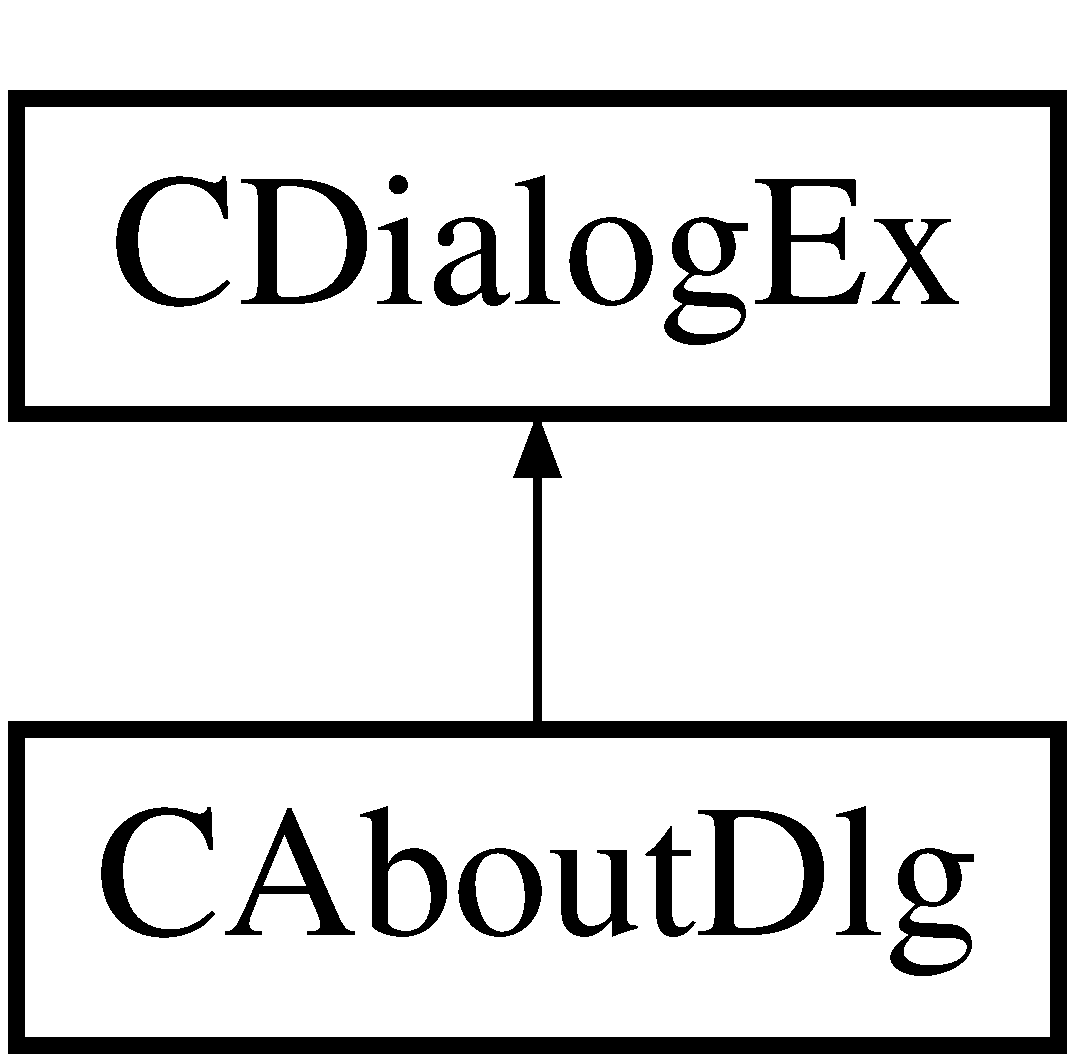
\includegraphics[height=2.000000cm]{class_c_about_dlg}
\end{center}
\end{figure}
\subsection*{Public 타입}
\begin{DoxyCompactItemize}
\item 
enum \{ \hyperlink{class_c_about_dlg_ab29e21bead9ca10b63b4628e8f8e4325ab6703c7538518b2b788243189e9f7981}{I\-D\-D} = I\-D\-D\-\_\-\-A\-B\-O\-U\-T\-B\-O\-X
 \}
\end{DoxyCompactItemize}
\subsection*{Public 멤버 함수}
\begin{DoxyCompactItemize}
\item 
\hyperlink{class_c_about_dlg_a6d1e6a33fef23bee6e75254189d865ce}{C\-About\-Dlg} ()
\end{DoxyCompactItemize}
\subsection*{Protected 멤버 함수}
\begin{DoxyCompactItemize}
\item 
virtual void \hyperlink{class_c_about_dlg_ab83db7484fec957282d7d5a21aed4df4}{Do\-Data\-Exchange} (C\-Data\-Exchange $\ast$p\-D\-X)
\end{DoxyCompactItemize}


\subsection{멤버 열거형 문서화}
\hypertarget{class_c_about_dlg_ab29e21bead9ca10b63b4628e8f8e4325}{\subsubsection[{anonymous enum}]{\setlength{\rightskip}{0pt plus 5cm}anonymous enum}}\label{class_c_about_dlg_ab29e21bead9ca10b63b4628e8f8e4325}
\begin{Desc}
\item[열거형 멤버\-: ]\par
\begin{description}
\index{I\-D\-D@{I\-D\-D}!C\-About\-Dlg@{C\-About\-Dlg}}\index{C\-About\-Dlg@{C\-About\-Dlg}!I\-D\-D@{I\-D\-D}}\item[{\em 
\hypertarget{class_c_about_dlg_ab29e21bead9ca10b63b4628e8f8e4325ab6703c7538518b2b788243189e9f7981}{I\-D\-D}\label{class_c_about_dlg_ab29e21bead9ca10b63b4628e8f8e4325ab6703c7538518b2b788243189e9f7981}
}]\end{description}
\end{Desc}



\subsection{생성자 \& 소멸자 문서화}
\hypertarget{class_c_about_dlg_a6d1e6a33fef23bee6e75254189d865ce}{\index{C\-About\-Dlg@{C\-About\-Dlg}!C\-About\-Dlg@{C\-About\-Dlg}}
\index{C\-About\-Dlg@{C\-About\-Dlg}!CAboutDlg@{C\-About\-Dlg}}
\subsubsection[{C\-About\-Dlg}]{\setlength{\rightskip}{0pt plus 5cm}C\-About\-Dlg\-::\-C\-About\-Dlg (
\begin{DoxyParamCaption}
{}
\end{DoxyParamCaption}
)}}\label{class_c_about_dlg_a6d1e6a33fef23bee6e75254189d865ce}


\subsection{멤버 함수 문서화}
\hypertarget{class_c_about_dlg_ab83db7484fec957282d7d5a21aed4df4}{\index{C\-About\-Dlg@{C\-About\-Dlg}!Do\-Data\-Exchange@{Do\-Data\-Exchange}}
\index{Do\-Data\-Exchange@{Do\-Data\-Exchange}!CAboutDlg@{C\-About\-Dlg}}
\subsubsection[{Do\-Data\-Exchange}]{\setlength{\rightskip}{0pt plus 5cm}void C\-About\-Dlg\-::\-Do\-Data\-Exchange (
\begin{DoxyParamCaption}
\item[{C\-Data\-Exchange $\ast$}]{p\-D\-X}
\end{DoxyParamCaption}
)\hspace{0.3cm}{\ttfamily [protected]}, {\ttfamily [virtual]}}}\label{class_c_about_dlg_ab83db7484fec957282d7d5a21aed4df4}


이 클래스에 대한 문서화 페이지는 다음의 파일로부터 생성되었습니다.\-:\begin{DoxyCompactItemize}
\item 
H\-:/\-Repository/\-My\-Image\-Processing/\-My\-Image\-Processing/\hyperlink{_my_image_processing_8cpp}{My\-Image\-Processing.\-cpp}\end{DoxyCompactItemize}

\hypertarget{class_c_binth_set}{\section{C\-Binth\-Set 클래스 참조}
\label{class_c_binth_set}\index{C\-Binth\-Set@{C\-Binth\-Set}}
}


{\ttfamily \#include $<$Binth\-Set.\-h$>$}

C\-Binth\-Set에 대한 상속 다이어그램 \-: \begin{figure}[H]
\begin{center}
\leavevmode
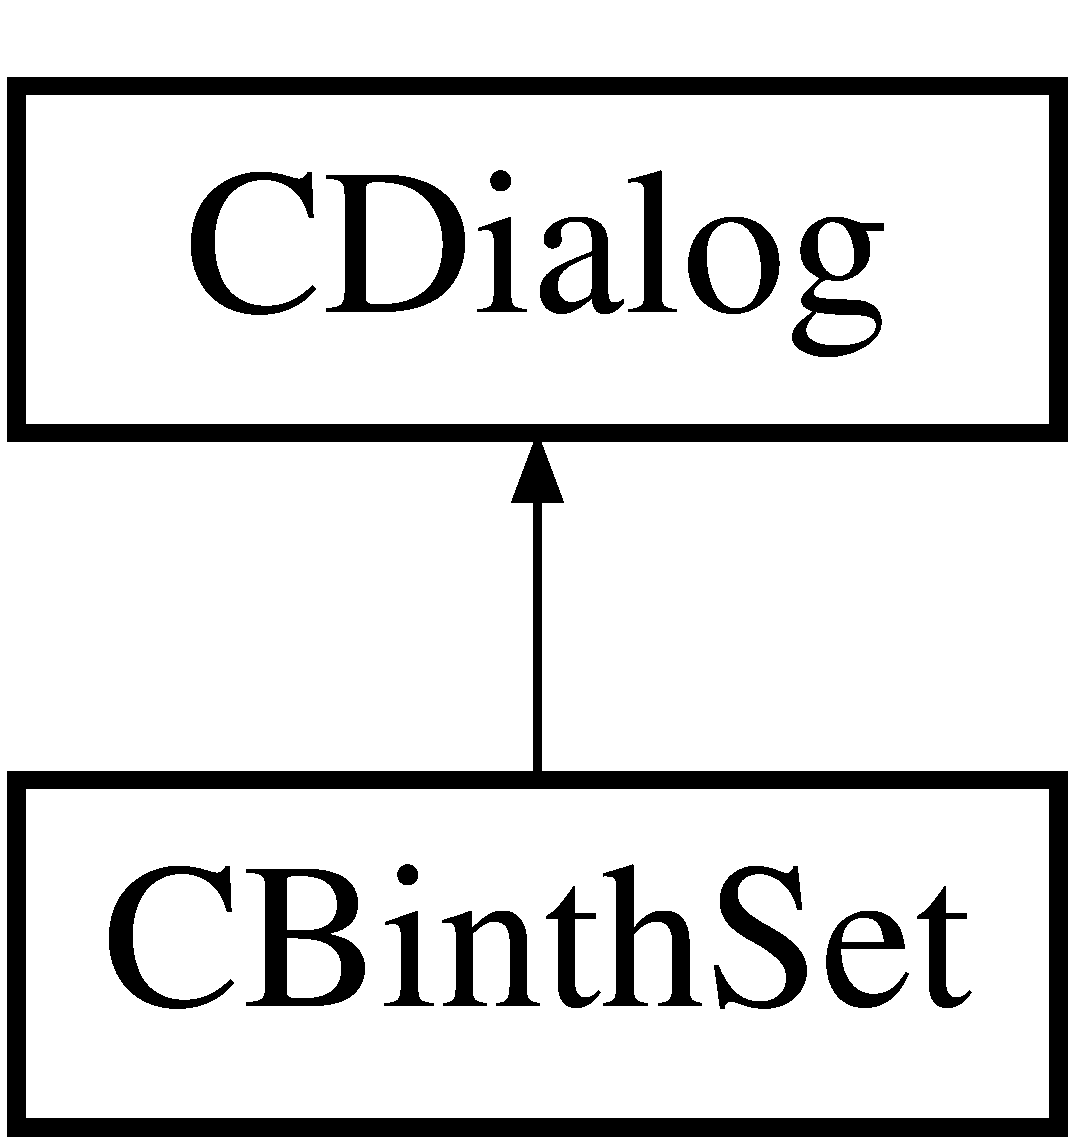
\includegraphics[height=2.000000cm]{class_c_binth_set}
\end{center}
\end{figure}
\subsection*{Public 타입}
\begin{DoxyCompactItemize}
\item 
enum \{ \hyperlink{class_c_binth_set_aca68a0fab0b7b10ebe4fd14a8a6c8c54a9d704acbd71024f8a51ae396d202392d}{I\-D\-D} = I\-D\-D\-\_\-\-B\-I\-N\-\_\-\-D\-L\-G
 \}
\end{DoxyCompactItemize}
\subsection*{Public 멤버 함수}
\begin{DoxyCompactItemize}
\item 
\hyperlink{class_c_binth_set_a3e8d4b627eea7c34e4779323dc6398fb}{C\-Binth\-Set} (C\-Wnd $\ast$p\-Parent=N\-U\-L\-L)
\item 
virtual \hyperlink{class_c_binth_set_aa9d7aa54a9308bc3a8c330f5289c4912}{$\sim$\-C\-Binth\-Set} ()
\item 
afx\-\_\-msg void \hyperlink{class_c_binth_set_a35f30f579e72fc9593335e620065aa15}{On\-Bn\-Clicked\-Ok} ()
\end{DoxyCompactItemize}
\subsection*{Public 속성}
\begin{DoxyCompactItemize}
\item 
int \hyperlink{class_c_binth_set_aa81e0016e3e463a022dbbaa6c7f85f2a}{m\-\_\-binth}
\end{DoxyCompactItemize}
\subsection*{Protected 멤버 함수}
\begin{DoxyCompactItemize}
\item 
virtual void \hyperlink{class_c_binth_set_ae150a279770f1fe4f597b73c07e887ba}{Do\-Data\-Exchange} (C\-Data\-Exchange $\ast$p\-D\-X)
\end{DoxyCompactItemize}


\subsection{멤버 열거형 문서화}
\hypertarget{class_c_binth_set_aca68a0fab0b7b10ebe4fd14a8a6c8c54}{\subsubsection[{anonymous enum}]{\setlength{\rightskip}{0pt plus 5cm}anonymous enum}}\label{class_c_binth_set_aca68a0fab0b7b10ebe4fd14a8a6c8c54}
\begin{Desc}
\item[열거형 멤버\-: ]\par
\begin{description}
\index{I\-D\-D@{I\-D\-D}!C\-Binth\-Set@{C\-Binth\-Set}}\index{C\-Binth\-Set@{C\-Binth\-Set}!I\-D\-D@{I\-D\-D}}\item[{\em 
\hypertarget{class_c_binth_set_aca68a0fab0b7b10ebe4fd14a8a6c8c54a9d704acbd71024f8a51ae396d202392d}{I\-D\-D}\label{class_c_binth_set_aca68a0fab0b7b10ebe4fd14a8a6c8c54a9d704acbd71024f8a51ae396d202392d}
}]\end{description}
\end{Desc}



\subsection{생성자 \& 소멸자 문서화}
\hypertarget{class_c_binth_set_a3e8d4b627eea7c34e4779323dc6398fb}{\index{C\-Binth\-Set@{C\-Binth\-Set}!C\-Binth\-Set@{C\-Binth\-Set}}
\index{C\-Binth\-Set@{C\-Binth\-Set}!CBinthSet@{C\-Binth\-Set}}
\subsubsection[{C\-Binth\-Set}]{\setlength{\rightskip}{0pt plus 5cm}C\-Binth\-Set\-::\-C\-Binth\-Set (
\begin{DoxyParamCaption}
\item[{C\-Wnd $\ast$}]{p\-Parent = {\ttfamily NULL}}
\end{DoxyParamCaption}
)}}\label{class_c_binth_set_a3e8d4b627eea7c34e4779323dc6398fb}
\hypertarget{class_c_binth_set_aa9d7aa54a9308bc3a8c330f5289c4912}{\index{C\-Binth\-Set@{C\-Binth\-Set}!$\sim$\-C\-Binth\-Set@{$\sim$\-C\-Binth\-Set}}
\index{$\sim$\-C\-Binth\-Set@{$\sim$\-C\-Binth\-Set}!CBinthSet@{C\-Binth\-Set}}
\subsubsection[{$\sim$\-C\-Binth\-Set}]{\setlength{\rightskip}{0pt plus 5cm}C\-Binth\-Set\-::$\sim$\-C\-Binth\-Set (
\begin{DoxyParamCaption}
{}
\end{DoxyParamCaption}
)\hspace{0.3cm}{\ttfamily [virtual]}}}\label{class_c_binth_set_aa9d7aa54a9308bc3a8c330f5289c4912}


\subsection{멤버 함수 문서화}
\hypertarget{class_c_binth_set_ae150a279770f1fe4f597b73c07e887ba}{\index{C\-Binth\-Set@{C\-Binth\-Set}!Do\-Data\-Exchange@{Do\-Data\-Exchange}}
\index{Do\-Data\-Exchange@{Do\-Data\-Exchange}!CBinthSet@{C\-Binth\-Set}}
\subsubsection[{Do\-Data\-Exchange}]{\setlength{\rightskip}{0pt plus 5cm}void C\-Binth\-Set\-::\-Do\-Data\-Exchange (
\begin{DoxyParamCaption}
\item[{C\-Data\-Exchange $\ast$}]{p\-D\-X}
\end{DoxyParamCaption}
)\hspace{0.3cm}{\ttfamily [protected]}, {\ttfamily [virtual]}}}\label{class_c_binth_set_ae150a279770f1fe4f597b73c07e887ba}
\hypertarget{class_c_binth_set_a35f30f579e72fc9593335e620065aa15}{\index{C\-Binth\-Set@{C\-Binth\-Set}!On\-Bn\-Clicked\-Ok@{On\-Bn\-Clicked\-Ok}}
\index{On\-Bn\-Clicked\-Ok@{On\-Bn\-Clicked\-Ok}!CBinthSet@{C\-Binth\-Set}}
\subsubsection[{On\-Bn\-Clicked\-Ok}]{\setlength{\rightskip}{0pt plus 5cm}void C\-Binth\-Set\-::\-On\-Bn\-Clicked\-Ok (
\begin{DoxyParamCaption}
{}
\end{DoxyParamCaption}
)}}\label{class_c_binth_set_a35f30f579e72fc9593335e620065aa15}


\subsection{멤버 데이타 문서화}
\hypertarget{class_c_binth_set_aa81e0016e3e463a022dbbaa6c7f85f2a}{\index{C\-Binth\-Set@{C\-Binth\-Set}!m\-\_\-binth@{m\-\_\-binth}}
\index{m\-\_\-binth@{m\-\_\-binth}!CBinthSet@{C\-Binth\-Set}}
\subsubsection[{m\-\_\-binth}]{\setlength{\rightskip}{0pt plus 5cm}int C\-Binth\-Set\-::m\-\_\-binth}}\label{class_c_binth_set_aa81e0016e3e463a022dbbaa6c7f85f2a}


이 클래스에 대한 문서화 페이지는 다음의 파일들로부터 생성되었습니다.\-:\begin{DoxyCompactItemize}
\item 
H\-:/\-Repository/\-My\-Image\-Processing/\-My\-Image\-Processing/\hyperlink{_binth_set_8h}{Binth\-Set.\-h}\item 
H\-:/\-Repository/\-My\-Image\-Processing/\-My\-Image\-Processing/\hyperlink{_binth_set_8cpp}{Binth\-Set.\-cpp}\end{DoxyCompactItemize}

\hypertarget{class_c_child_frame}{\section{C\-Child\-Frame 클래스 참조}
\label{class_c_child_frame}\index{C\-Child\-Frame@{C\-Child\-Frame}}
}


{\ttfamily \#include $<$Child\-Frm.\-h$>$}

C\-Child\-Frame에 대한 상속 다이어그램 \-: \begin{figure}[H]
\begin{center}
\leavevmode
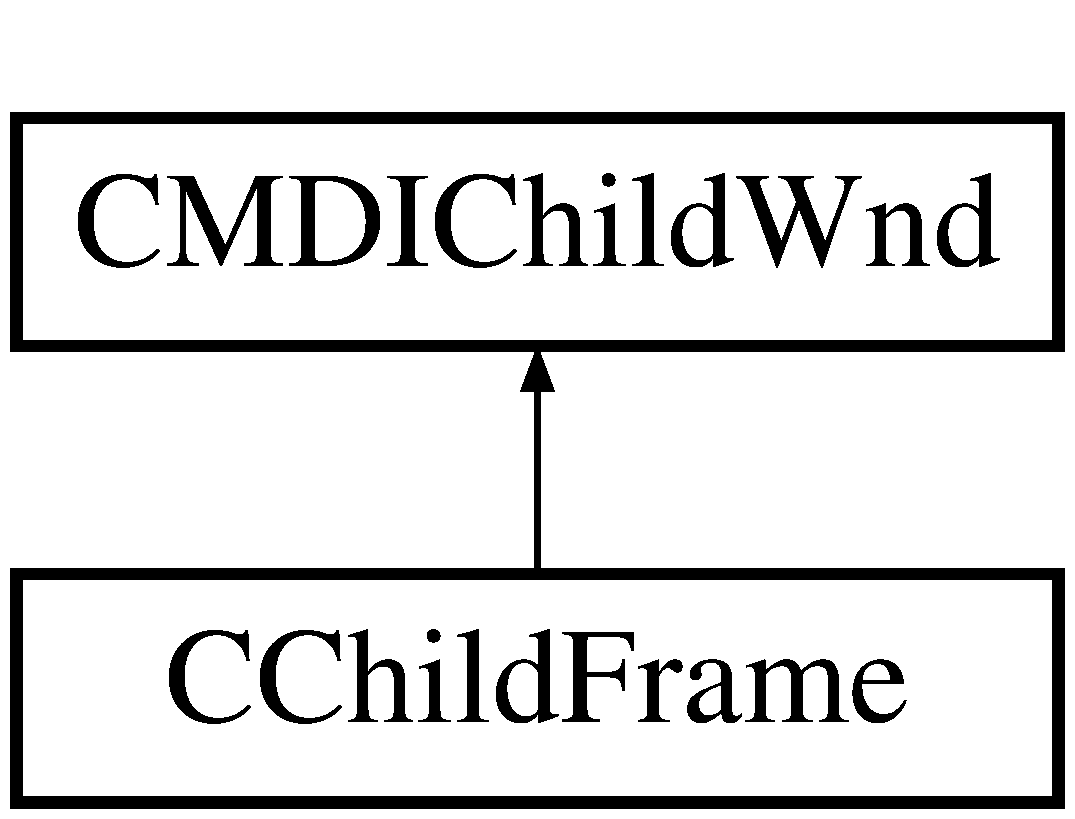
\includegraphics[height=2.000000cm]{class_c_child_frame}
\end{center}
\end{figure}
\subsection*{Public 멤버 함수}
\begin{DoxyCompactItemize}
\item 
\hyperlink{class_c_child_frame_ac25f19634b6795d77ef5b739900232d6}{C\-Child\-Frame} ()
\item 
virtual B\-O\-O\-L \hyperlink{class_c_child_frame_afe5999283ada65f5b1f9fbabb288a8fe}{Pre\-Create\-Window} (C\-R\-E\-A\-T\-E\-S\-T\-R\-U\-C\-T \&cs)
\item 
virtual \hyperlink{class_c_child_frame_ae43d3b449c8696c96963d0818de69735}{$\sim$\-C\-Child\-Frame} ()
\end{DoxyCompactItemize}


\subsection{생성자 \& 소멸자 문서화}
\hypertarget{class_c_child_frame_ac25f19634b6795d77ef5b739900232d6}{\index{C\-Child\-Frame@{C\-Child\-Frame}!C\-Child\-Frame@{C\-Child\-Frame}}
\index{C\-Child\-Frame@{C\-Child\-Frame}!CChildFrame@{C\-Child\-Frame}}
\subsubsection[{C\-Child\-Frame}]{\setlength{\rightskip}{0pt plus 5cm}C\-Child\-Frame\-::\-C\-Child\-Frame (
\begin{DoxyParamCaption}
{}
\end{DoxyParamCaption}
)}}\label{class_c_child_frame_ac25f19634b6795d77ef5b739900232d6}
\hypertarget{class_c_child_frame_ae43d3b449c8696c96963d0818de69735}{\index{C\-Child\-Frame@{C\-Child\-Frame}!$\sim$\-C\-Child\-Frame@{$\sim$\-C\-Child\-Frame}}
\index{$\sim$\-C\-Child\-Frame@{$\sim$\-C\-Child\-Frame}!CChildFrame@{C\-Child\-Frame}}
\subsubsection[{$\sim$\-C\-Child\-Frame}]{\setlength{\rightskip}{0pt plus 5cm}C\-Child\-Frame\-::$\sim$\-C\-Child\-Frame (
\begin{DoxyParamCaption}
{}
\end{DoxyParamCaption}
)\hspace{0.3cm}{\ttfamily [virtual]}}}\label{class_c_child_frame_ae43d3b449c8696c96963d0818de69735}


\subsection{멤버 함수 문서화}
\hypertarget{class_c_child_frame_afe5999283ada65f5b1f9fbabb288a8fe}{\index{C\-Child\-Frame@{C\-Child\-Frame}!Pre\-Create\-Window@{Pre\-Create\-Window}}
\index{Pre\-Create\-Window@{Pre\-Create\-Window}!CChildFrame@{C\-Child\-Frame}}
\subsubsection[{Pre\-Create\-Window}]{\setlength{\rightskip}{0pt plus 5cm}B\-O\-O\-L C\-Child\-Frame\-::\-Pre\-Create\-Window (
\begin{DoxyParamCaption}
\item[{C\-R\-E\-A\-T\-E\-S\-T\-R\-U\-C\-T \&}]{cs}
\end{DoxyParamCaption}
)\hspace{0.3cm}{\ttfamily [virtual]}}}\label{class_c_child_frame_afe5999283ada65f5b1f9fbabb288a8fe}


이 클래스에 대한 문서화 페이지는 다음의 파일들로부터 생성되었습니다.\-:\begin{DoxyCompactItemize}
\item 
H\-:/\-Repository/\-My\-Image\-Processing/\-My\-Image\-Processing/\hyperlink{_child_frm_8h}{Child\-Frm.\-h}\item 
H\-:/\-Repository/\-My\-Image\-Processing/\-My\-Image\-Processing/\hyperlink{_child_frm_8cpp}{Child\-Frm.\-cpp}\end{DoxyCompactItemize}

\hypertarget{class_c_h_b_dlg}{\section{C\-H\-B\-Dlg 클래스 참조}
\label{class_c_h_b_dlg}\index{C\-H\-B\-Dlg@{C\-H\-B\-Dlg}}
}


{\ttfamily \#include $<$H\-B\-Dlg.\-h$>$}

C\-H\-B\-Dlg에 대한 상속 다이어그램 \-: \begin{figure}[H]
\begin{center}
\leavevmode
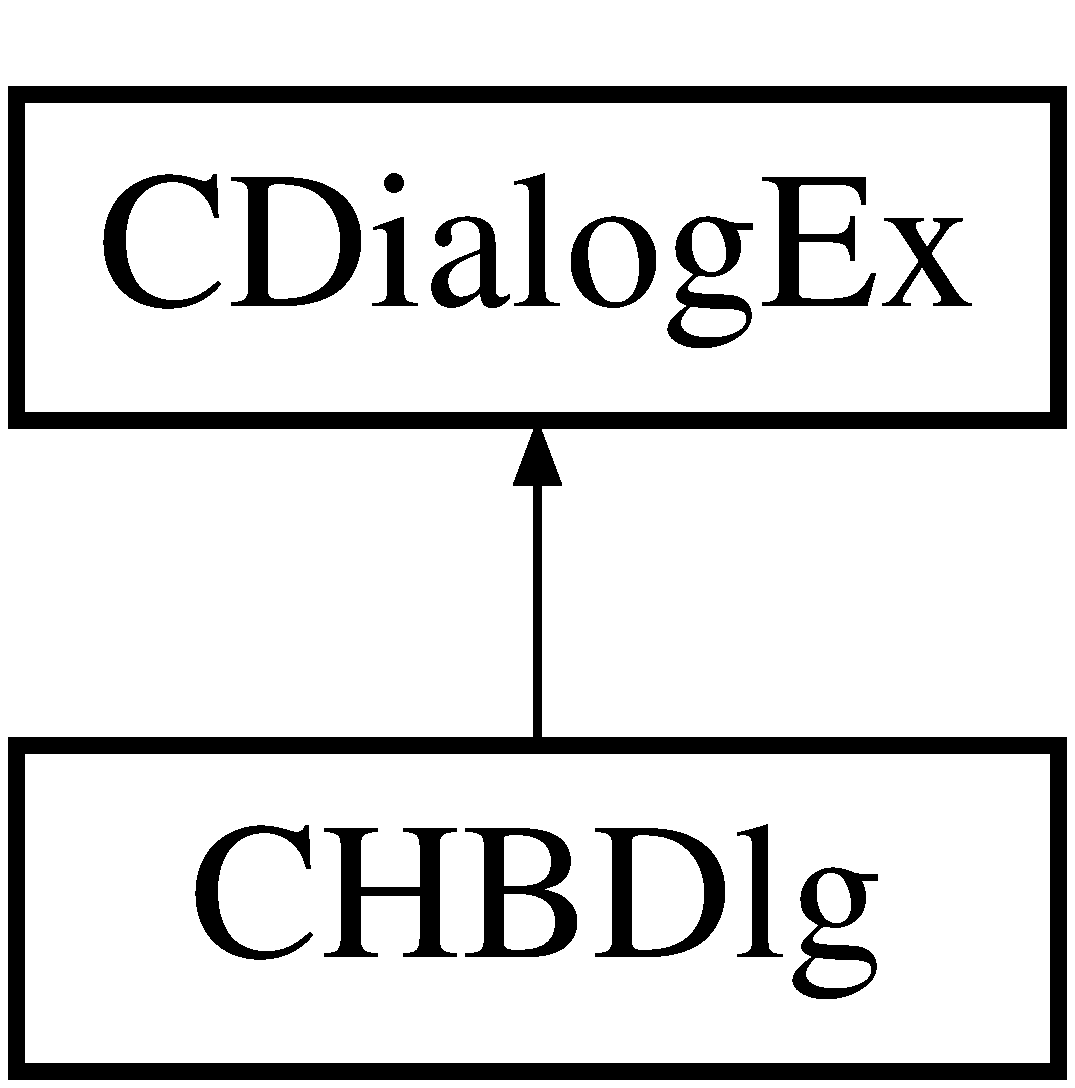
\includegraphics[height=2.000000cm]{class_c_h_b_dlg}
\end{center}
\end{figure}
\subsection*{Public 타입}
\begin{DoxyCompactItemize}
\item 
enum \{ \hyperlink{class_c_h_b_dlg_a85c548c902dee40ffff4a0ab6abf026ea551e8b24bba5583d8430cdec070fdd90}{I\-D\-D} = I\-D\-D\-\_\-\-H\-B\-\_\-\-D\-L\-G
 \}
\end{DoxyCompactItemize}
\subsection*{Public 멤버 함수}
\begin{DoxyCompactItemize}
\item 
\hyperlink{class_c_h_b_dlg_ad1ad2d7431f683474b3e674a758e45cf}{C\-H\-B\-Dlg} (C\-Wnd $\ast$p\-Parent=N\-U\-L\-L)
\item 
virtual \hyperlink{class_c_h_b_dlg_aa6fa7e090e4b39b162e071867acad12e}{$\sim$\-C\-H\-B\-Dlg} ()
\end{DoxyCompactItemize}
\subsection*{Public 속성}
\begin{DoxyCompactItemize}
\item 
double \hyperlink{class_c_h_b_dlg_a9df17f6054e5bd5e4acfabe606fc12b3}{m\-\_\-\-A}
\end{DoxyCompactItemize}
\subsection*{Protected 멤버 함수}
\begin{DoxyCompactItemize}
\item 
virtual void \hyperlink{class_c_h_b_dlg_a4a5143405ebecad3bbc6e32dcc0b0f9b}{Do\-Data\-Exchange} (C\-Data\-Exchange $\ast$p\-D\-X)
\end{DoxyCompactItemize}


\subsection{멤버 열거형 문서화}
\hypertarget{class_c_h_b_dlg_a85c548c902dee40ffff4a0ab6abf026e}{\subsubsection[{anonymous enum}]{\setlength{\rightskip}{0pt plus 5cm}anonymous enum}}\label{class_c_h_b_dlg_a85c548c902dee40ffff4a0ab6abf026e}
\begin{Desc}
\item[열거형 멤버\-: ]\par
\begin{description}
\index{I\-D\-D@{I\-D\-D}!C\-H\-B\-Dlg@{C\-H\-B\-Dlg}}\index{C\-H\-B\-Dlg@{C\-H\-B\-Dlg}!I\-D\-D@{I\-D\-D}}\item[{\em 
\hypertarget{class_c_h_b_dlg_a85c548c902dee40ffff4a0ab6abf026ea551e8b24bba5583d8430cdec070fdd90}{I\-D\-D}\label{class_c_h_b_dlg_a85c548c902dee40ffff4a0ab6abf026ea551e8b24bba5583d8430cdec070fdd90}
}]\end{description}
\end{Desc}



\subsection{생성자 \& 소멸자 문서화}
\hypertarget{class_c_h_b_dlg_ad1ad2d7431f683474b3e674a758e45cf}{\index{C\-H\-B\-Dlg@{C\-H\-B\-Dlg}!C\-H\-B\-Dlg@{C\-H\-B\-Dlg}}
\index{C\-H\-B\-Dlg@{C\-H\-B\-Dlg}!CHBDlg@{C\-H\-B\-Dlg}}
\subsubsection[{C\-H\-B\-Dlg}]{\setlength{\rightskip}{0pt plus 5cm}C\-H\-B\-Dlg\-::\-C\-H\-B\-Dlg (
\begin{DoxyParamCaption}
\item[{C\-Wnd $\ast$}]{p\-Parent = {\ttfamily NULL}}
\end{DoxyParamCaption}
)}}\label{class_c_h_b_dlg_ad1ad2d7431f683474b3e674a758e45cf}
\hypertarget{class_c_h_b_dlg_aa6fa7e090e4b39b162e071867acad12e}{\index{C\-H\-B\-Dlg@{C\-H\-B\-Dlg}!$\sim$\-C\-H\-B\-Dlg@{$\sim$\-C\-H\-B\-Dlg}}
\index{$\sim$\-C\-H\-B\-Dlg@{$\sim$\-C\-H\-B\-Dlg}!CHBDlg@{C\-H\-B\-Dlg}}
\subsubsection[{$\sim$\-C\-H\-B\-Dlg}]{\setlength{\rightskip}{0pt plus 5cm}C\-H\-B\-Dlg\-::$\sim$\-C\-H\-B\-Dlg (
\begin{DoxyParamCaption}
{}
\end{DoxyParamCaption}
)\hspace{0.3cm}{\ttfamily [virtual]}}}\label{class_c_h_b_dlg_aa6fa7e090e4b39b162e071867acad12e}


\subsection{멤버 함수 문서화}
\hypertarget{class_c_h_b_dlg_a4a5143405ebecad3bbc6e32dcc0b0f9b}{\index{C\-H\-B\-Dlg@{C\-H\-B\-Dlg}!Do\-Data\-Exchange@{Do\-Data\-Exchange}}
\index{Do\-Data\-Exchange@{Do\-Data\-Exchange}!CHBDlg@{C\-H\-B\-Dlg}}
\subsubsection[{Do\-Data\-Exchange}]{\setlength{\rightskip}{0pt plus 5cm}void C\-H\-B\-Dlg\-::\-Do\-Data\-Exchange (
\begin{DoxyParamCaption}
\item[{C\-Data\-Exchange $\ast$}]{p\-D\-X}
\end{DoxyParamCaption}
)\hspace{0.3cm}{\ttfamily [protected]}, {\ttfamily [virtual]}}}\label{class_c_h_b_dlg_a4a5143405ebecad3bbc6e32dcc0b0f9b}


\subsection{멤버 데이타 문서화}
\hypertarget{class_c_h_b_dlg_a9df17f6054e5bd5e4acfabe606fc12b3}{\index{C\-H\-B\-Dlg@{C\-H\-B\-Dlg}!m\-\_\-\-A@{m\-\_\-\-A}}
\index{m\-\_\-\-A@{m\-\_\-\-A}!CHBDlg@{C\-H\-B\-Dlg}}
\subsubsection[{m\-\_\-\-A}]{\setlength{\rightskip}{0pt plus 5cm}double C\-H\-B\-Dlg\-::m\-\_\-\-A}}\label{class_c_h_b_dlg_a9df17f6054e5bd5e4acfabe606fc12b3}


이 클래스에 대한 문서화 페이지는 다음의 파일들로부터 생성되었습니다.\-:\begin{DoxyCompactItemize}
\item 
My\-Image\-Processing/\hyperlink{_h_b_dlg_8h}{H\-B\-Dlg.\-h}\item 
My\-Image\-Processing/\hyperlink{_h_b_dlg_8cpp}{H\-B\-Dlg.\-cpp}\end{DoxyCompactItemize}

\hypertarget{class_c_hist_dlg}{\section{C\-Hist\-Dlg 클래스 참조}
\label{class_c_hist_dlg}\index{C\-Hist\-Dlg@{C\-Hist\-Dlg}}
}


{\ttfamily \#include $<$Hist\-Dlg.\-h$>$}

C\-Hist\-Dlg에 대한 상속 다이어그램 \-: \begin{figure}[H]
\begin{center}
\leavevmode
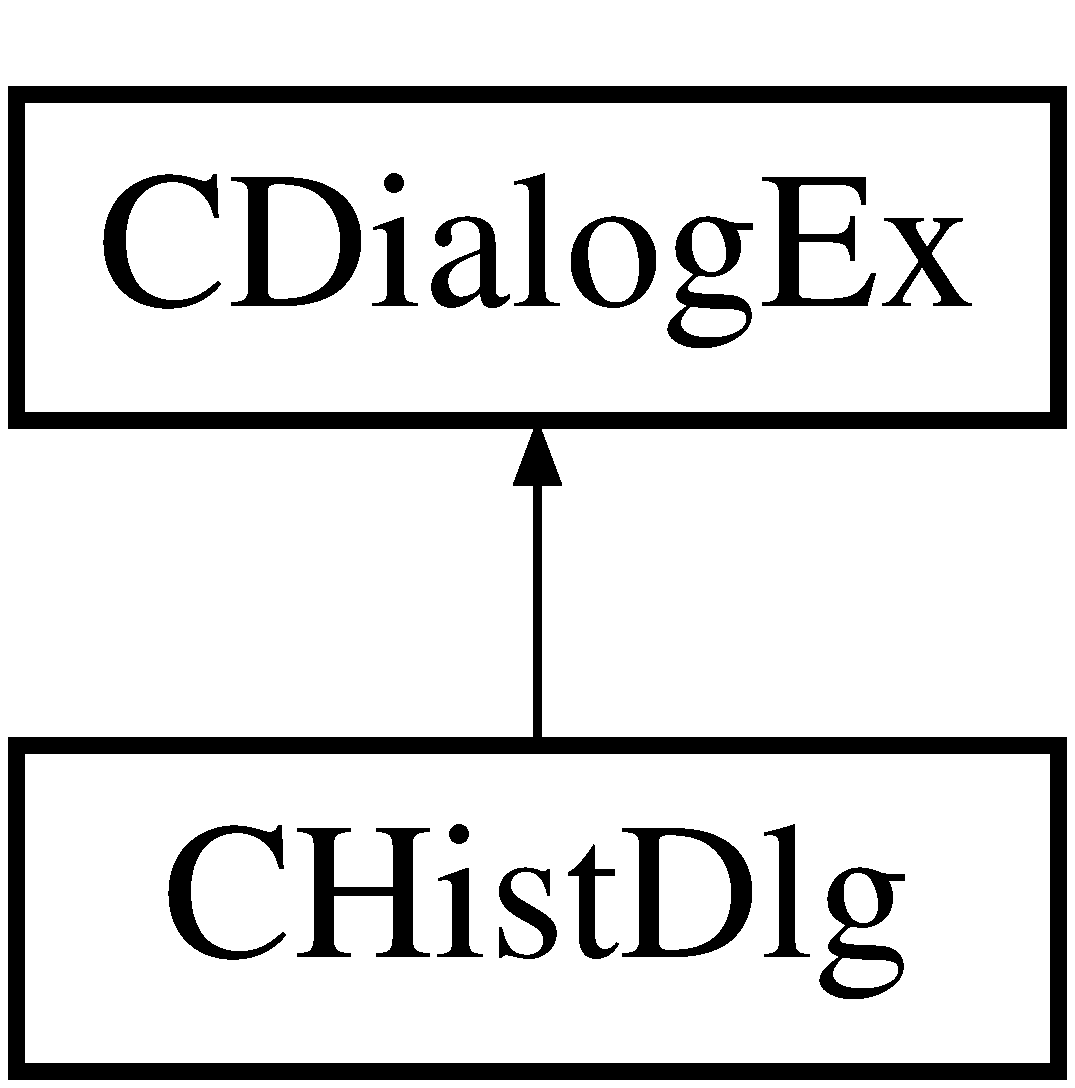
\includegraphics[height=2.000000cm]{class_c_hist_dlg}
\end{center}
\end{figure}
\subsection*{Public 타입}
\begin{DoxyCompactItemize}
\item 
enum \{ \hyperlink{class_c_hist_dlg_ac536fdef65118a44834ace1e795b5d53a6355bda489fa5ea40bdc03fb4ea1baea}{I\-D\-D} = I\-D\-D\-\_\-\-H\-I\-S\-T\-\_\-\-D\-L\-G
 \}
\end{DoxyCompactItemize}
\subsection*{Public 멤버 함수}
\begin{DoxyCompactItemize}
\item 
\hyperlink{class_c_hist_dlg_aa172ce29b9e60682f146391eff5fdce0}{C\-Hist\-Dlg} (C\-Wnd $\ast$p\-Parent=N\-U\-L\-L)
\item 
virtual \hyperlink{class_c_hist_dlg_a16e7c76fa6892cb0545974d62a089521}{$\sim$\-C\-Hist\-Dlg} ()
\item 
void \hyperlink{class_c_hist_dlg_a29a406cadf520060ad60a7a9a246ac57}{Set\-Image} (Cx\-Image $\ast$img, int k=0)
\item 
afx\-\_\-msg void \hyperlink{class_c_hist_dlg_ada0bb1f41d5042d24816802a405b064e}{On\-Paint} ()
\item 
afx\-\_\-msg void \hyperlink{class_c_hist_dlg_a9cf978b6cac92b42356db7e01502bd25}{On\-Bn\-Clicked\-Radio1} ()
\item 
afx\-\_\-msg void \hyperlink{class_c_hist_dlg_afddab2267513f03160832fb11491d58d}{On\-Bn\-Clicked\-Radio2} ()
\item 
afx\-\_\-msg void \hyperlink{class_c_hist_dlg_a1afa7ec674ebbe137b275d5c62f967db}{On\-Bn\-Clicked\-Radio3} ()
\item 
virtual B\-O\-O\-L \hyperlink{class_c_hist_dlg_ae655e453dd12a2ee5db4c1ab2bb57c88}{On\-Init\-Dialog} ()
\end{DoxyCompactItemize}
\subsection*{Protected 멤버 함수}
\begin{DoxyCompactItemize}
\item 
virtual void \hyperlink{class_c_hist_dlg_ad79b371c18c4129610b59608d97ed67f}{Do\-Data\-Exchange} (C\-Data\-Exchange $\ast$p\-D\-X)
\end{DoxyCompactItemize}
\subsection*{Private 속성}
\begin{DoxyCompactItemize}
\item 
double \hyperlink{class_c_hist_dlg_a6c2d395cebef6f871fd1791fa57b6f55}{m\-\_\-\-Histogram} \mbox{[}256\mbox{]}
\item 
Cx\-Image $\ast$ \hyperlink{class_c_hist_dlg_a931451fed18d5abe289575cecc8e9f54}{m\-\_\-img}
\end{DoxyCompactItemize}


\subsection{멤버 열거형 문서화}
\hypertarget{class_c_hist_dlg_ac536fdef65118a44834ace1e795b5d53}{\subsubsection[{anonymous enum}]{\setlength{\rightskip}{0pt plus 5cm}anonymous enum}}\label{class_c_hist_dlg_ac536fdef65118a44834ace1e795b5d53}
\begin{Desc}
\item[열거형 멤버\-: ]\par
\begin{description}
\index{I\-D\-D@{I\-D\-D}!C\-Hist\-Dlg@{C\-Hist\-Dlg}}\index{C\-Hist\-Dlg@{C\-Hist\-Dlg}!I\-D\-D@{I\-D\-D}}\item[{\em 
\hypertarget{class_c_hist_dlg_ac536fdef65118a44834ace1e795b5d53a6355bda489fa5ea40bdc03fb4ea1baea}{I\-D\-D}\label{class_c_hist_dlg_ac536fdef65118a44834ace1e795b5d53a6355bda489fa5ea40bdc03fb4ea1baea}
}]\end{description}
\end{Desc}



\subsection{생성자 \& 소멸자 문서화}
\hypertarget{class_c_hist_dlg_aa172ce29b9e60682f146391eff5fdce0}{\index{C\-Hist\-Dlg@{C\-Hist\-Dlg}!C\-Hist\-Dlg@{C\-Hist\-Dlg}}
\index{C\-Hist\-Dlg@{C\-Hist\-Dlg}!CHistDlg@{C\-Hist\-Dlg}}
\subsubsection[{C\-Hist\-Dlg}]{\setlength{\rightskip}{0pt plus 5cm}C\-Hist\-Dlg\-::\-C\-Hist\-Dlg (
\begin{DoxyParamCaption}
\item[{C\-Wnd $\ast$}]{p\-Parent = {\ttfamily NULL}}
\end{DoxyParamCaption}
)}}\label{class_c_hist_dlg_aa172ce29b9e60682f146391eff5fdce0}
\hypertarget{class_c_hist_dlg_a16e7c76fa6892cb0545974d62a089521}{\index{C\-Hist\-Dlg@{C\-Hist\-Dlg}!$\sim$\-C\-Hist\-Dlg@{$\sim$\-C\-Hist\-Dlg}}
\index{$\sim$\-C\-Hist\-Dlg@{$\sim$\-C\-Hist\-Dlg}!CHistDlg@{C\-Hist\-Dlg}}
\subsubsection[{$\sim$\-C\-Hist\-Dlg}]{\setlength{\rightskip}{0pt plus 5cm}C\-Hist\-Dlg\-::$\sim$\-C\-Hist\-Dlg (
\begin{DoxyParamCaption}
{}
\end{DoxyParamCaption}
)\hspace{0.3cm}{\ttfamily [virtual]}}}\label{class_c_hist_dlg_a16e7c76fa6892cb0545974d62a089521}


\subsection{멤버 함수 문서화}
\hypertarget{class_c_hist_dlg_ad79b371c18c4129610b59608d97ed67f}{\index{C\-Hist\-Dlg@{C\-Hist\-Dlg}!Do\-Data\-Exchange@{Do\-Data\-Exchange}}
\index{Do\-Data\-Exchange@{Do\-Data\-Exchange}!CHistDlg@{C\-Hist\-Dlg}}
\subsubsection[{Do\-Data\-Exchange}]{\setlength{\rightskip}{0pt plus 5cm}void C\-Hist\-Dlg\-::\-Do\-Data\-Exchange (
\begin{DoxyParamCaption}
\item[{C\-Data\-Exchange $\ast$}]{p\-D\-X}
\end{DoxyParamCaption}
)\hspace{0.3cm}{\ttfamily [protected]}, {\ttfamily [virtual]}}}\label{class_c_hist_dlg_ad79b371c18c4129610b59608d97ed67f}
\hypertarget{class_c_hist_dlg_a9cf978b6cac92b42356db7e01502bd25}{\index{C\-Hist\-Dlg@{C\-Hist\-Dlg}!On\-Bn\-Clicked\-Radio1@{On\-Bn\-Clicked\-Radio1}}
\index{On\-Bn\-Clicked\-Radio1@{On\-Bn\-Clicked\-Radio1}!CHistDlg@{C\-Hist\-Dlg}}
\subsubsection[{On\-Bn\-Clicked\-Radio1}]{\setlength{\rightskip}{0pt plus 5cm}void C\-Hist\-Dlg\-::\-On\-Bn\-Clicked\-Radio1 (
\begin{DoxyParamCaption}
{}
\end{DoxyParamCaption}
)}}\label{class_c_hist_dlg_a9cf978b6cac92b42356db7e01502bd25}
\hypertarget{class_c_hist_dlg_afddab2267513f03160832fb11491d58d}{\index{C\-Hist\-Dlg@{C\-Hist\-Dlg}!On\-Bn\-Clicked\-Radio2@{On\-Bn\-Clicked\-Radio2}}
\index{On\-Bn\-Clicked\-Radio2@{On\-Bn\-Clicked\-Radio2}!CHistDlg@{C\-Hist\-Dlg}}
\subsubsection[{On\-Bn\-Clicked\-Radio2}]{\setlength{\rightskip}{0pt plus 5cm}void C\-Hist\-Dlg\-::\-On\-Bn\-Clicked\-Radio2 (
\begin{DoxyParamCaption}
{}
\end{DoxyParamCaption}
)}}\label{class_c_hist_dlg_afddab2267513f03160832fb11491d58d}
\hypertarget{class_c_hist_dlg_a1afa7ec674ebbe137b275d5c62f967db}{\index{C\-Hist\-Dlg@{C\-Hist\-Dlg}!On\-Bn\-Clicked\-Radio3@{On\-Bn\-Clicked\-Radio3}}
\index{On\-Bn\-Clicked\-Radio3@{On\-Bn\-Clicked\-Radio3}!CHistDlg@{C\-Hist\-Dlg}}
\subsubsection[{On\-Bn\-Clicked\-Radio3}]{\setlength{\rightskip}{0pt plus 5cm}void C\-Hist\-Dlg\-::\-On\-Bn\-Clicked\-Radio3 (
\begin{DoxyParamCaption}
{}
\end{DoxyParamCaption}
)}}\label{class_c_hist_dlg_a1afa7ec674ebbe137b275d5c62f967db}
\hypertarget{class_c_hist_dlg_ae655e453dd12a2ee5db4c1ab2bb57c88}{\index{C\-Hist\-Dlg@{C\-Hist\-Dlg}!On\-Init\-Dialog@{On\-Init\-Dialog}}
\index{On\-Init\-Dialog@{On\-Init\-Dialog}!CHistDlg@{C\-Hist\-Dlg}}
\subsubsection[{On\-Init\-Dialog}]{\setlength{\rightskip}{0pt plus 5cm}B\-O\-O\-L C\-Hist\-Dlg\-::\-On\-Init\-Dialog (
\begin{DoxyParamCaption}
{}
\end{DoxyParamCaption}
)\hspace{0.3cm}{\ttfamily [virtual]}}}\label{class_c_hist_dlg_ae655e453dd12a2ee5db4c1ab2bb57c88}
\hypertarget{class_c_hist_dlg_ada0bb1f41d5042d24816802a405b064e}{\index{C\-Hist\-Dlg@{C\-Hist\-Dlg}!On\-Paint@{On\-Paint}}
\index{On\-Paint@{On\-Paint}!CHistDlg@{C\-Hist\-Dlg}}
\subsubsection[{On\-Paint}]{\setlength{\rightskip}{0pt plus 5cm}void C\-Hist\-Dlg\-::\-On\-Paint (
\begin{DoxyParamCaption}
{}
\end{DoxyParamCaption}
)}}\label{class_c_hist_dlg_ada0bb1f41d5042d24816802a405b064e}
\hypertarget{class_c_hist_dlg_a29a406cadf520060ad60a7a9a246ac57}{\index{C\-Hist\-Dlg@{C\-Hist\-Dlg}!Set\-Image@{Set\-Image}}
\index{Set\-Image@{Set\-Image}!CHistDlg@{C\-Hist\-Dlg}}
\subsubsection[{Set\-Image}]{\setlength{\rightskip}{0pt plus 5cm}void C\-Hist\-Dlg\-::\-Set\-Image (
\begin{DoxyParamCaption}
\item[{Cx\-Image $\ast$}]{img, }
\item[{int}]{k = {\ttfamily 0}}
\end{DoxyParamCaption}
)}}\label{class_c_hist_dlg_a29a406cadf520060ad60a7a9a246ac57}


\subsection{멤버 데이타 문서화}
\hypertarget{class_c_hist_dlg_a6c2d395cebef6f871fd1791fa57b6f55}{\index{C\-Hist\-Dlg@{C\-Hist\-Dlg}!m\-\_\-\-Histogram@{m\-\_\-\-Histogram}}
\index{m\-\_\-\-Histogram@{m\-\_\-\-Histogram}!CHistDlg@{C\-Hist\-Dlg}}
\subsubsection[{m\-\_\-\-Histogram}]{\setlength{\rightskip}{0pt plus 5cm}double C\-Hist\-Dlg\-::m\-\_\-\-Histogram\mbox{[}256\mbox{]}\hspace{0.3cm}{\ttfamily [private]}}}\label{class_c_hist_dlg_a6c2d395cebef6f871fd1791fa57b6f55}
\hypertarget{class_c_hist_dlg_a931451fed18d5abe289575cecc8e9f54}{\index{C\-Hist\-Dlg@{C\-Hist\-Dlg}!m\-\_\-img@{m\-\_\-img}}
\index{m\-\_\-img@{m\-\_\-img}!CHistDlg@{C\-Hist\-Dlg}}
\subsubsection[{m\-\_\-img}]{\setlength{\rightskip}{0pt plus 5cm}Cx\-Image$\ast$ C\-Hist\-Dlg\-::m\-\_\-img\hspace{0.3cm}{\ttfamily [private]}}}\label{class_c_hist_dlg_a931451fed18d5abe289575cecc8e9f54}


이 클래스에 대한 문서화 페이지는 다음의 파일들로부터 생성되었습니다.\-:\begin{DoxyCompactItemize}
\item 
H\-:/\-Repository/\-My\-Image\-Processing/\-My\-Image\-Processing/\hyperlink{_hist_dlg_8h}{Hist\-Dlg.\-h}\item 
H\-:/\-Repository/\-My\-Image\-Processing/\-My\-Image\-Processing/\hyperlink{_hist_dlg_8cpp}{Hist\-Dlg.\-cpp}\end{DoxyCompactItemize}

\hypertarget{class_c_main_frame}{\section{C\-Main\-Frame 클래스 참조}
\label{class_c_main_frame}\index{C\-Main\-Frame@{C\-Main\-Frame}}
}


{\ttfamily \#include $<$Main\-Frm.\-h$>$}

C\-Main\-Frame에 대한 상속 다이어그램 \-: \begin{figure}[H]
\begin{center}
\leavevmode
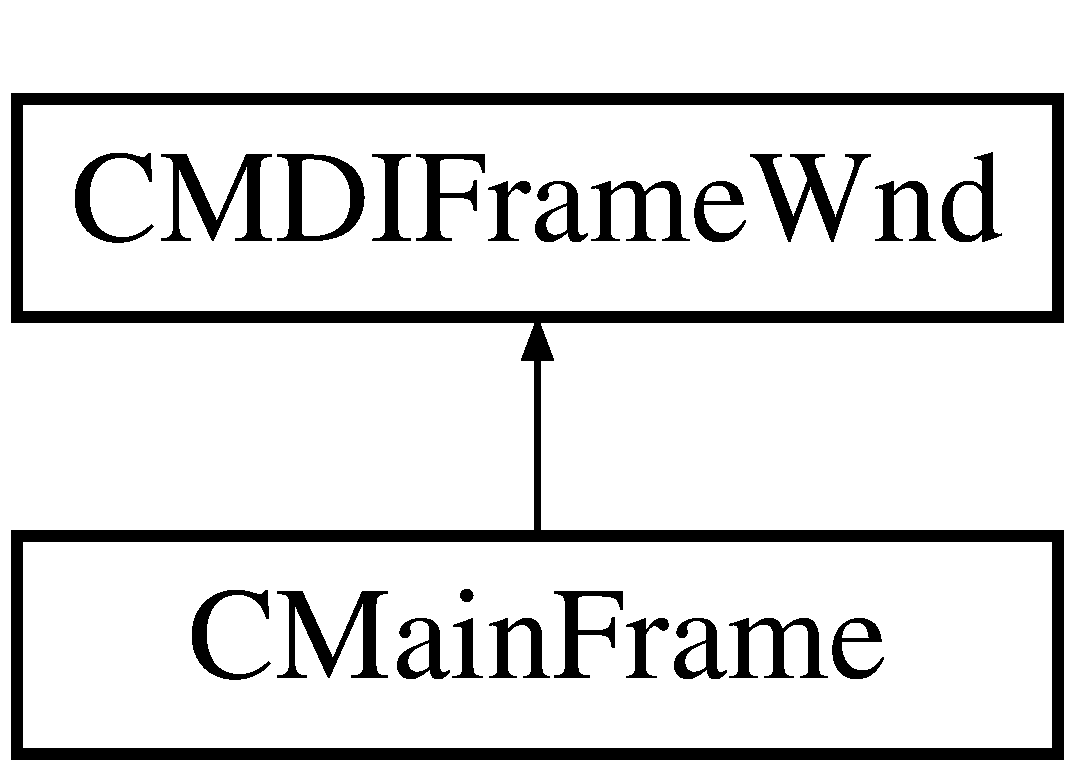
\includegraphics[height=2.000000cm]{class_c_main_frame}
\end{center}
\end{figure}
\subsection*{Public 멤버 함수}
\begin{DoxyCompactItemize}
\item 
\hyperlink{class_c_main_frame_af3e997aeae4148d2aaa4a1e1ae7bdd53}{C\-Main\-Frame} ()
\item 
virtual B\-O\-O\-L \hyperlink{class_c_main_frame_a549bf677c955c2898c3c683321633c16}{Pre\-Create\-Window} (C\-R\-E\-A\-T\-E\-S\-T\-R\-U\-C\-T \&cs)
\item 
virtual \hyperlink{class_c_main_frame_a8ae555f23fdf97edb4feb4d3e1bfa4ee}{$\sim$\-C\-Main\-Frame} ()
\end{DoxyCompactItemize}
\subsection*{Protected 멤버 함수}
\begin{DoxyCompactItemize}
\item 
afx\-\_\-msg int \hyperlink{class_c_main_frame_a48666466fd37412fcaeff75c3b12e0ed}{On\-Create} (L\-P\-C\-R\-E\-A\-T\-E\-S\-T\-R\-U\-C\-T lp\-Create\-Struct)
\end{DoxyCompactItemize}
\subsection*{Protected 속성}
\begin{DoxyCompactItemize}
\item 
C\-Status\-Bar \hyperlink{class_c_main_frame_ac01bafc03aee69cf982e6f029b4db6b0}{m\-\_\-wnd\-Status\-Bar}
\end{DoxyCompactItemize}


\subsection{생성자 \& 소멸자 문서화}
\hypertarget{class_c_main_frame_af3e997aeae4148d2aaa4a1e1ae7bdd53}{\index{C\-Main\-Frame@{C\-Main\-Frame}!C\-Main\-Frame@{C\-Main\-Frame}}
\index{C\-Main\-Frame@{C\-Main\-Frame}!CMainFrame@{C\-Main\-Frame}}
\subsubsection[{C\-Main\-Frame}]{\setlength{\rightskip}{0pt plus 5cm}C\-Main\-Frame\-::\-C\-Main\-Frame (
\begin{DoxyParamCaption}
{}
\end{DoxyParamCaption}
)}}\label{class_c_main_frame_af3e997aeae4148d2aaa4a1e1ae7bdd53}
\hypertarget{class_c_main_frame_a8ae555f23fdf97edb4feb4d3e1bfa4ee}{\index{C\-Main\-Frame@{C\-Main\-Frame}!$\sim$\-C\-Main\-Frame@{$\sim$\-C\-Main\-Frame}}
\index{$\sim$\-C\-Main\-Frame@{$\sim$\-C\-Main\-Frame}!CMainFrame@{C\-Main\-Frame}}
\subsubsection[{$\sim$\-C\-Main\-Frame}]{\setlength{\rightskip}{0pt plus 5cm}C\-Main\-Frame\-::$\sim$\-C\-Main\-Frame (
\begin{DoxyParamCaption}
{}
\end{DoxyParamCaption}
)\hspace{0.3cm}{\ttfamily [virtual]}}}\label{class_c_main_frame_a8ae555f23fdf97edb4feb4d3e1bfa4ee}


\subsection{멤버 함수 문서화}
\hypertarget{class_c_main_frame_a48666466fd37412fcaeff75c3b12e0ed}{\index{C\-Main\-Frame@{C\-Main\-Frame}!On\-Create@{On\-Create}}
\index{On\-Create@{On\-Create}!CMainFrame@{C\-Main\-Frame}}
\subsubsection[{On\-Create}]{\setlength{\rightskip}{0pt plus 5cm}int C\-Main\-Frame\-::\-On\-Create (
\begin{DoxyParamCaption}
\item[{L\-P\-C\-R\-E\-A\-T\-E\-S\-T\-R\-U\-C\-T}]{lp\-Create\-Struct}
\end{DoxyParamCaption}
)\hspace{0.3cm}{\ttfamily [protected]}}}\label{class_c_main_frame_a48666466fd37412fcaeff75c3b12e0ed}
\hypertarget{class_c_main_frame_a549bf677c955c2898c3c683321633c16}{\index{C\-Main\-Frame@{C\-Main\-Frame}!Pre\-Create\-Window@{Pre\-Create\-Window}}
\index{Pre\-Create\-Window@{Pre\-Create\-Window}!CMainFrame@{C\-Main\-Frame}}
\subsubsection[{Pre\-Create\-Window}]{\setlength{\rightskip}{0pt plus 5cm}B\-O\-O\-L C\-Main\-Frame\-::\-Pre\-Create\-Window (
\begin{DoxyParamCaption}
\item[{C\-R\-E\-A\-T\-E\-S\-T\-R\-U\-C\-T \&}]{cs}
\end{DoxyParamCaption}
)\hspace{0.3cm}{\ttfamily [virtual]}}}\label{class_c_main_frame_a549bf677c955c2898c3c683321633c16}


\subsection{멤버 데이타 문서화}
\hypertarget{class_c_main_frame_ac01bafc03aee69cf982e6f029b4db6b0}{\index{C\-Main\-Frame@{C\-Main\-Frame}!m\-\_\-wnd\-Status\-Bar@{m\-\_\-wnd\-Status\-Bar}}
\index{m\-\_\-wnd\-Status\-Bar@{m\-\_\-wnd\-Status\-Bar}!CMainFrame@{C\-Main\-Frame}}
\subsubsection[{m\-\_\-wnd\-Status\-Bar}]{\setlength{\rightskip}{0pt plus 5cm}C\-Status\-Bar C\-Main\-Frame\-::m\-\_\-wnd\-Status\-Bar\hspace{0.3cm}{\ttfamily [protected]}}}\label{class_c_main_frame_ac01bafc03aee69cf982e6f029b4db6b0}


이 클래스에 대한 문서화 페이지는 다음의 파일들로부터 생성되었습니다.\-:\begin{DoxyCompactItemize}
\item 
My\-Image\-Processing/\hyperlink{_main_frm_8h}{Main\-Frm.\-h}\item 
My\-Image\-Processing/\hyperlink{_main_frm_8cpp}{Main\-Frm.\-cpp}\end{DoxyCompactItemize}

\hypertarget{class_c_my_image_processing_app}{\section{C\-My\-Image\-Processing\-App 클래스 참조}
\label{class_c_my_image_processing_app}\index{C\-My\-Image\-Processing\-App@{C\-My\-Image\-Processing\-App}}
}


{\ttfamily \#include $<$My\-Image\-Processing.\-h$>$}

C\-My\-Image\-Processing\-App에 대한 상속 다이어그램 \-: \begin{figure}[H]
\begin{center}
\leavevmode
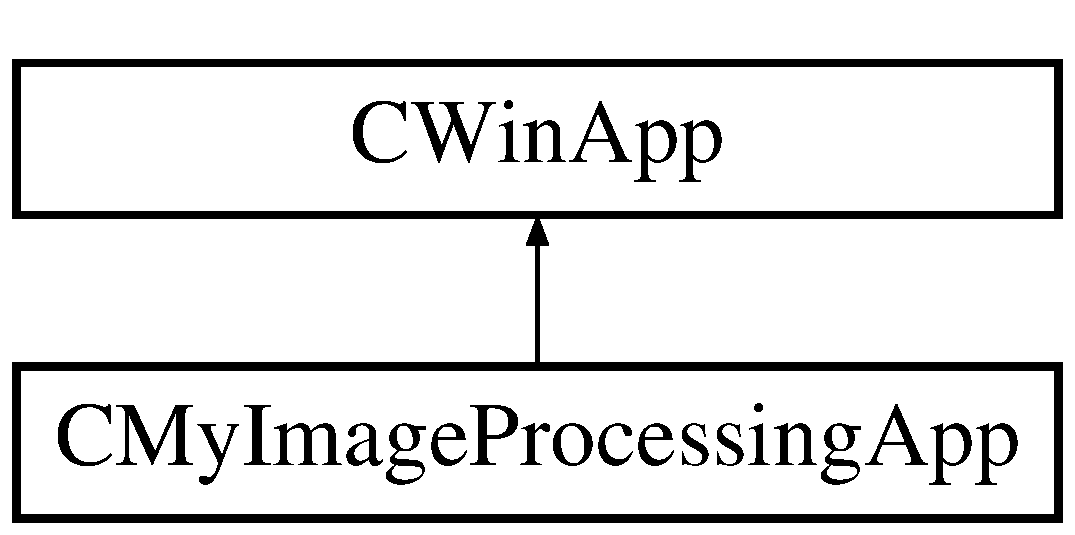
\includegraphics[height=2.000000cm]{class_c_my_image_processing_app}
\end{center}
\end{figure}
\subsection*{Public 멤버 함수}
\begin{DoxyCompactItemize}
\item 
\hyperlink{class_c_my_image_processing_app_ad1f80d98d11ebd682d96f4f242a1ac8e}{C\-My\-Image\-Processing\-App} ()
\item 
virtual B\-O\-O\-L \hyperlink{class_c_my_image_processing_app_a39dbd1c72587d475ba844ace08463174}{Init\-Instance} ()
\item 
virtual int \hyperlink{class_c_my_image_processing_app_aa9f926c482433d072c7594667a685fef}{Exit\-Instance} ()
\item 
afx\-\_\-msg void \hyperlink{class_c_my_image_processing_app_ad29a277fd0fba00c3fd4dfecc47a2eca}{On\-App\-About} ()
\end{DoxyCompactItemize}
\subsection*{Public 속성}
\begin{DoxyCompactItemize}
\item 
Cx\-Image $\ast$ \hyperlink{class_c_my_image_processing_app_ad42155c6a3d9aad19b57bb15a06ddda9}{m\-\_\-p\-New\-Image}
\item 
\hyperlink{class_my_image}{My\-Image} $\ast$ \hyperlink{class_c_my_image_processing_app_aa5a25236bb1a996bb2c86864d54fba25}{m\-\_\-\-New\-Image}
\end{DoxyCompactItemize}


\subsection{생성자 \& 소멸자 문서화}
\hypertarget{class_c_my_image_processing_app_ad1f80d98d11ebd682d96f4f242a1ac8e}{\index{C\-My\-Image\-Processing\-App@{C\-My\-Image\-Processing\-App}!C\-My\-Image\-Processing\-App@{C\-My\-Image\-Processing\-App}}
\index{C\-My\-Image\-Processing\-App@{C\-My\-Image\-Processing\-App}!CMyImageProcessingApp@{C\-My\-Image\-Processing\-App}}
\subsubsection[{C\-My\-Image\-Processing\-App}]{\setlength{\rightskip}{0pt plus 5cm}C\-My\-Image\-Processing\-App\-::\-C\-My\-Image\-Processing\-App (
\begin{DoxyParamCaption}
{}
\end{DoxyParamCaption}
)}}\label{class_c_my_image_processing_app_ad1f80d98d11ebd682d96f4f242a1ac8e}


\subsection{멤버 함수 문서화}
\hypertarget{class_c_my_image_processing_app_aa9f926c482433d072c7594667a685fef}{\index{C\-My\-Image\-Processing\-App@{C\-My\-Image\-Processing\-App}!Exit\-Instance@{Exit\-Instance}}
\index{Exit\-Instance@{Exit\-Instance}!CMyImageProcessingApp@{C\-My\-Image\-Processing\-App}}
\subsubsection[{Exit\-Instance}]{\setlength{\rightskip}{0pt plus 5cm}int C\-My\-Image\-Processing\-App\-::\-Exit\-Instance (
\begin{DoxyParamCaption}
{}
\end{DoxyParamCaption}
)\hspace{0.3cm}{\ttfamily [virtual]}}}\label{class_c_my_image_processing_app_aa9f926c482433d072c7594667a685fef}
\hypertarget{class_c_my_image_processing_app_a39dbd1c72587d475ba844ace08463174}{\index{C\-My\-Image\-Processing\-App@{C\-My\-Image\-Processing\-App}!Init\-Instance@{Init\-Instance}}
\index{Init\-Instance@{Init\-Instance}!CMyImageProcessingApp@{C\-My\-Image\-Processing\-App}}
\subsubsection[{Init\-Instance}]{\setlength{\rightskip}{0pt plus 5cm}B\-O\-O\-L C\-My\-Image\-Processing\-App\-::\-Init\-Instance (
\begin{DoxyParamCaption}
{}
\end{DoxyParamCaption}
)\hspace{0.3cm}{\ttfamily [virtual]}}}\label{class_c_my_image_processing_app_a39dbd1c72587d475ba844ace08463174}
\hypertarget{class_c_my_image_processing_app_ad29a277fd0fba00c3fd4dfecc47a2eca}{\index{C\-My\-Image\-Processing\-App@{C\-My\-Image\-Processing\-App}!On\-App\-About@{On\-App\-About}}
\index{On\-App\-About@{On\-App\-About}!CMyImageProcessingApp@{C\-My\-Image\-Processing\-App}}
\subsubsection[{On\-App\-About}]{\setlength{\rightskip}{0pt plus 5cm}void C\-My\-Image\-Processing\-App\-::\-On\-App\-About (
\begin{DoxyParamCaption}
{}
\end{DoxyParamCaption}
)}}\label{class_c_my_image_processing_app_ad29a277fd0fba00c3fd4dfecc47a2eca}


\subsection{멤버 데이타 문서화}
\hypertarget{class_c_my_image_processing_app_aa5a25236bb1a996bb2c86864d54fba25}{\index{C\-My\-Image\-Processing\-App@{C\-My\-Image\-Processing\-App}!m\-\_\-\-New\-Image@{m\-\_\-\-New\-Image}}
\index{m\-\_\-\-New\-Image@{m\-\_\-\-New\-Image}!CMyImageProcessingApp@{C\-My\-Image\-Processing\-App}}
\subsubsection[{m\-\_\-\-New\-Image}]{\setlength{\rightskip}{0pt plus 5cm}{\bf My\-Image}$\ast$ C\-My\-Image\-Processing\-App\-::m\-\_\-\-New\-Image}}\label{class_c_my_image_processing_app_aa5a25236bb1a996bb2c86864d54fba25}
\hypertarget{class_c_my_image_processing_app_ad42155c6a3d9aad19b57bb15a06ddda9}{\index{C\-My\-Image\-Processing\-App@{C\-My\-Image\-Processing\-App}!m\-\_\-p\-New\-Image@{m\-\_\-p\-New\-Image}}
\index{m\-\_\-p\-New\-Image@{m\-\_\-p\-New\-Image}!CMyImageProcessingApp@{C\-My\-Image\-Processing\-App}}
\subsubsection[{m\-\_\-p\-New\-Image}]{\setlength{\rightskip}{0pt plus 5cm}Cx\-Image$\ast$ C\-My\-Image\-Processing\-App\-::m\-\_\-p\-New\-Image}}\label{class_c_my_image_processing_app_ad42155c6a3d9aad19b57bb15a06ddda9}


이 클래스에 대한 문서화 페이지는 다음의 파일들로부터 생성되었습니다.\-:\begin{DoxyCompactItemize}
\item 
My\-Image\-Processing/\hyperlink{_my_image_processing_8h}{My\-Image\-Processing.\-h}\item 
My\-Image\-Processing/\hyperlink{_my_image_processing_8cpp}{My\-Image\-Processing.\-cpp}\end{DoxyCompactItemize}

\hypertarget{class_c_my_image_processing_doc}{\section{C\-My\-Image\-Processing\-Doc 클래스 참조}
\label{class_c_my_image_processing_doc}\index{C\-My\-Image\-Processing\-Doc@{C\-My\-Image\-Processing\-Doc}}
}


{\ttfamily \#include $<$My\-Image\-Processing\-Doc.\-h$>$}

C\-My\-Image\-Processing\-Doc에 대한 상속 다이어그램 \-: \begin{figure}[H]
\begin{center}
\leavevmode
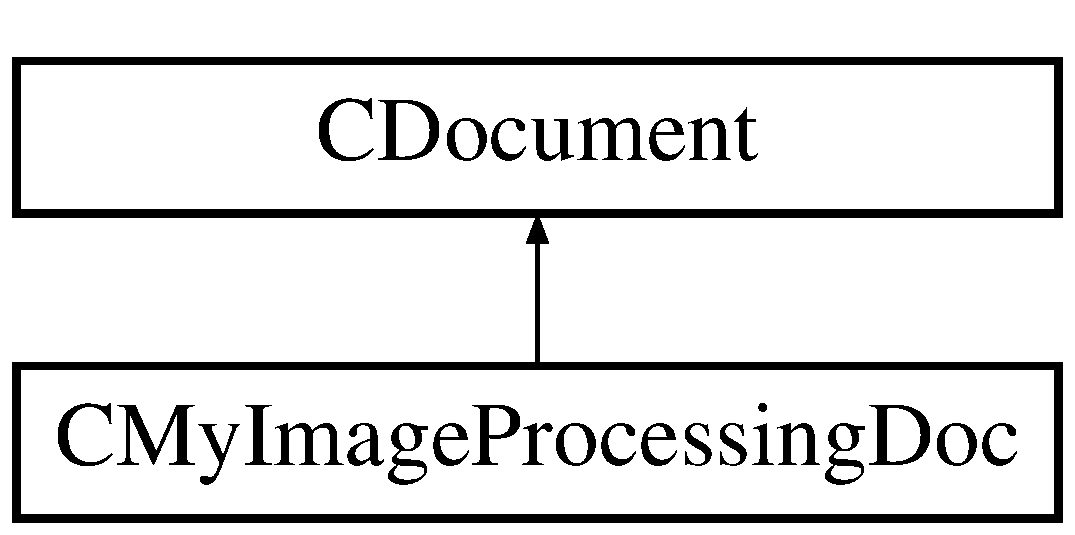
\includegraphics[height=2.000000cm]{class_c_my_image_processing_doc}
\end{center}
\end{figure}
\subsection*{Public 멤버 함수}
\begin{DoxyCompactItemize}
\item 
virtual B\-O\-O\-L \hyperlink{class_c_my_image_processing_doc_ace51febeb853241b30e372aeec5c736c}{On\-New\-Document} ()
\item 
virtual void \hyperlink{class_c_my_image_processing_doc_afccbabdc62acc9c794684f19ba91706c}{Serialize} (C\-Archive \&ar)
\item 
virtual \hyperlink{class_c_my_image_processing_doc_af38a8ca89b352f41e050415e15f4414a}{$\sim$\-C\-My\-Image\-Processing\-Doc} ()
\item 
void \hyperlink{class_c_my_image_processing_doc_a6b945ff1dea330304876d455efbce925}{View\-Image} (\hyperlink{class_my_image}{My\-Image} \&img)
\item 
virtual B\-O\-O\-L \hyperlink{class_c_my_image_processing_doc_a298ff63e6cf66c8e034a1b23439e36a0}{On\-Open\-Document} (L\-P\-C\-T\-S\-T\-R lpsz\-Path\-Name)
\item 
virtual void \hyperlink{class_c_my_image_processing_doc_a27823ce295ac534756ddd1c5c672c963}{Delete\-Contents} ()
\item 
virtual B\-O\-O\-L \hyperlink{class_c_my_image_processing_doc_a462530f8b6ba55216a02afd079e54a85}{On\-Save\-Document} (L\-P\-C\-T\-S\-T\-R lpsz\-Path\-Name)
\item 
afx\-\_\-msg void \hyperlink{class_c_my_image_processing_doc_a3922aa78dfd3a645704b51650716bc5d}{On\-Img\-Gray} ()
\item 
afx\-\_\-msg void \hyperlink{class_c_my_image_processing_doc_adf46e407c93d02b63a668c7ac5089d57}{On\-Img\-Inv} ()
\item 
afx\-\_\-msg void \hyperlink{class_c_my_image_processing_doc_a222391b07cb5517c953f291975d3a4ae}{On\-Img\-Bin} ()
\item 
afx\-\_\-msg void \hyperlink{class_c_my_image_processing_doc_ac3eb4d895a330361dfc6dfcdb48c9437}{On\-Img\-Scl} ()
\item 
afx\-\_\-msg void \hyperlink{class_c_my_image_processing_doc_a224d7b1fc7bcf0f034e5e0b3d46c186e}{On\-Hist} ()
\item 
afx\-\_\-msg void \hyperlink{class_c_my_image_processing_doc_a5f3fbe7ce6035ae4837adc633517ade2}{On\-Hist\-Eq} ()
\item 
afx\-\_\-msg void \hyperlink{class_c_my_image_processing_doc_a8d8f9f5aacf4200ccb0047aa1afd949a}{On\-Laplacion} ()
\item 
int \hyperlink{class_c_my_image_processing_doc_a541cb66c2473454a49be669acaa0db67}{calc\-Mask} (double mask\mbox{[}$\,$\mbox{]}\mbox{[}3\mbox{]}, int x, int y, int k)
\item 
afx\-\_\-msg void \hyperlink{class_c_my_image_processing_doc_a02adaf0fa2601aa7257403f3add15d45}{On\-High\-Boost} ()
\item 
afx\-\_\-msg void \hyperlink{class_c_my_image_processing_doc_ae1eb87303d441fee44eee9cc0713f35e}{On\-Sobel} ()
\item 
afx\-\_\-msg void \hyperlink{class_c_my_image_processing_doc_a81bf8bfe13998034c311facb4480b72a}{On\-Sm\-Lin} ()
\item 
afx\-\_\-msg void \hyperlink{class_c_my_image_processing_doc_ae19b8ec98c48bb0092cd6d49a4365870}{On\-Order\-Maxfilter} ()
\item 
afx\-\_\-msg void \hyperlink{class_c_my_image_processing_doc_a179bd964abd852b3276b536e6d1cbfaa}{On\-Order\-Medianfilter} ()
\item 
afx\-\_\-msg void \hyperlink{class_c_my_image_processing_doc_a086368f43f1bdca128134b4397942516}{On\-Order\-Minfilter} ()
\item 
afx\-\_\-msg void \hyperlink{class_c_my_image_processing_doc_afdc7a9e36d9ec2d9f600737ed67a31d7}{On\-Polar\-Trans} ()
\item 
afx\-\_\-msg void \hyperlink{class_c_my_image_processing_doc_a2ce4f7dce9e33b9bb7baf5cfc908b516}{On\-Polar\-Trans\-Inv} ()
\item 
afx\-\_\-msg void \hyperlink{class_c_my_image_processing_doc_a7798d32dd4e007b2f92a4cfd17863660}{On\-Cartesian\-Trans} ()
\item 
afx\-\_\-msg void \hyperlink{class_c_my_image_processing_doc_a59e47774204f909d57cbb86b12a2d0ab}{On\-Power} ()
\item 
afx\-\_\-msg void \hyperlink{class_c_my_image_processing_doc_acc6818171d5d567884143cdd10a5cb25}{On\-Order\-Meanfilter} ()
\item 
afx\-\_\-msg void \hyperlink{class_c_my_image_processing_doc_a739a32984fd9a5c759cf940772b092ac}{On\-Fft} ()
\item 
afx\-\_\-msg void \hyperlink{class_c_my_image_processing_doc_a4663dab53118f156bca90aaefa2f6058}{On\-Dft} ()
\end{DoxyCompactItemize}
\subsection*{Public 속성}
\begin{DoxyCompactItemize}
\item 
Cx\-Image $\ast$ \hyperlink{class_c_my_image_processing_doc_ad5fdd82c16f80240fb27e6f3a04a333b}{m\-\_\-p\-Image}
\item 
\hyperlink{class_my_image}{My\-Image} $\ast$ \hyperlink{class_c_my_image_processing_doc_a4f70944ed5cc5c772165aec9a9e88c69}{m\-\_\-\-Image}
\end{DoxyCompactItemize}
\subsection*{Protected 멤버 함수}
\begin{DoxyCompactItemize}
\item 
\hyperlink{class_c_my_image_processing_doc_a9ec11e938f149d2669d791c89772e5ac}{C\-My\-Image\-Processing\-Doc} ()
\end{DoxyCompactItemize}


\subsection{생성자 \& 소멸자 문서화}
\hypertarget{class_c_my_image_processing_doc_a9ec11e938f149d2669d791c89772e5ac}{\index{C\-My\-Image\-Processing\-Doc@{C\-My\-Image\-Processing\-Doc}!C\-My\-Image\-Processing\-Doc@{C\-My\-Image\-Processing\-Doc}}
\index{C\-My\-Image\-Processing\-Doc@{C\-My\-Image\-Processing\-Doc}!CMyImageProcessingDoc@{C\-My\-Image\-Processing\-Doc}}
\subsubsection[{C\-My\-Image\-Processing\-Doc}]{\setlength{\rightskip}{0pt plus 5cm}C\-My\-Image\-Processing\-Doc\-::\-C\-My\-Image\-Processing\-Doc (
\begin{DoxyParamCaption}
{}
\end{DoxyParamCaption}
)\hspace{0.3cm}{\ttfamily [protected]}}}\label{class_c_my_image_processing_doc_a9ec11e938f149d2669d791c89772e5ac}
\hypertarget{class_c_my_image_processing_doc_af38a8ca89b352f41e050415e15f4414a}{\index{C\-My\-Image\-Processing\-Doc@{C\-My\-Image\-Processing\-Doc}!$\sim$\-C\-My\-Image\-Processing\-Doc@{$\sim$\-C\-My\-Image\-Processing\-Doc}}
\index{$\sim$\-C\-My\-Image\-Processing\-Doc@{$\sim$\-C\-My\-Image\-Processing\-Doc}!CMyImageProcessingDoc@{C\-My\-Image\-Processing\-Doc}}
\subsubsection[{$\sim$\-C\-My\-Image\-Processing\-Doc}]{\setlength{\rightskip}{0pt plus 5cm}C\-My\-Image\-Processing\-Doc\-::$\sim$\-C\-My\-Image\-Processing\-Doc (
\begin{DoxyParamCaption}
{}
\end{DoxyParamCaption}
)\hspace{0.3cm}{\ttfamily [virtual]}}}\label{class_c_my_image_processing_doc_af38a8ca89b352f41e050415e15f4414a}


\subsection{멤버 함수 문서화}
\hypertarget{class_c_my_image_processing_doc_a541cb66c2473454a49be669acaa0db67}{\index{C\-My\-Image\-Processing\-Doc@{C\-My\-Image\-Processing\-Doc}!calc\-Mask@{calc\-Mask}}
\index{calc\-Mask@{calc\-Mask}!CMyImageProcessingDoc@{C\-My\-Image\-Processing\-Doc}}
\subsubsection[{calc\-Mask}]{\setlength{\rightskip}{0pt plus 5cm}int C\-My\-Image\-Processing\-Doc\-::calc\-Mask (
\begin{DoxyParamCaption}
\item[{double}]{mask\mbox{[}$\,$\mbox{]}\mbox{[}3\mbox{]}, }
\item[{int}]{x, }
\item[{int}]{y, }
\item[{int}]{k}
\end{DoxyParamCaption}
)}}\label{class_c_my_image_processing_doc_a541cb66c2473454a49be669acaa0db67}
\hypertarget{class_c_my_image_processing_doc_a27823ce295ac534756ddd1c5c672c963}{\index{C\-My\-Image\-Processing\-Doc@{C\-My\-Image\-Processing\-Doc}!Delete\-Contents@{Delete\-Contents}}
\index{Delete\-Contents@{Delete\-Contents}!CMyImageProcessingDoc@{C\-My\-Image\-Processing\-Doc}}
\subsubsection[{Delete\-Contents}]{\setlength{\rightskip}{0pt plus 5cm}void C\-My\-Image\-Processing\-Doc\-::\-Delete\-Contents (
\begin{DoxyParamCaption}
{}
\end{DoxyParamCaption}
)\hspace{0.3cm}{\ttfamily [virtual]}}}\label{class_c_my_image_processing_doc_a27823ce295ac534756ddd1c5c672c963}
\hypertarget{class_c_my_image_processing_doc_a7798d32dd4e007b2f92a4cfd17863660}{\index{C\-My\-Image\-Processing\-Doc@{C\-My\-Image\-Processing\-Doc}!On\-Cartesian\-Trans@{On\-Cartesian\-Trans}}
\index{On\-Cartesian\-Trans@{On\-Cartesian\-Trans}!CMyImageProcessingDoc@{C\-My\-Image\-Processing\-Doc}}
\subsubsection[{On\-Cartesian\-Trans}]{\setlength{\rightskip}{0pt plus 5cm}void C\-My\-Image\-Processing\-Doc\-::\-On\-Cartesian\-Trans (
\begin{DoxyParamCaption}
{}
\end{DoxyParamCaption}
)}}\label{class_c_my_image_processing_doc_a7798d32dd4e007b2f92a4cfd17863660}
\hypertarget{class_c_my_image_processing_doc_a4663dab53118f156bca90aaefa2f6058}{\index{C\-My\-Image\-Processing\-Doc@{C\-My\-Image\-Processing\-Doc}!On\-Dft@{On\-Dft}}
\index{On\-Dft@{On\-Dft}!CMyImageProcessingDoc@{C\-My\-Image\-Processing\-Doc}}
\subsubsection[{On\-Dft}]{\setlength{\rightskip}{0pt plus 5cm}void C\-My\-Image\-Processing\-Doc\-::\-On\-Dft (
\begin{DoxyParamCaption}
{}
\end{DoxyParamCaption}
)}}\label{class_c_my_image_processing_doc_a4663dab53118f156bca90aaefa2f6058}
\hypertarget{class_c_my_image_processing_doc_a739a32984fd9a5c759cf940772b092ac}{\index{C\-My\-Image\-Processing\-Doc@{C\-My\-Image\-Processing\-Doc}!On\-Fft@{On\-Fft}}
\index{On\-Fft@{On\-Fft}!CMyImageProcessingDoc@{C\-My\-Image\-Processing\-Doc}}
\subsubsection[{On\-Fft}]{\setlength{\rightskip}{0pt plus 5cm}void C\-My\-Image\-Processing\-Doc\-::\-On\-Fft (
\begin{DoxyParamCaption}
{}
\end{DoxyParamCaption}
)}}\label{class_c_my_image_processing_doc_a739a32984fd9a5c759cf940772b092ac}
\hypertarget{class_c_my_image_processing_doc_a02adaf0fa2601aa7257403f3add15d45}{\index{C\-My\-Image\-Processing\-Doc@{C\-My\-Image\-Processing\-Doc}!On\-High\-Boost@{On\-High\-Boost}}
\index{On\-High\-Boost@{On\-High\-Boost}!CMyImageProcessingDoc@{C\-My\-Image\-Processing\-Doc}}
\subsubsection[{On\-High\-Boost}]{\setlength{\rightskip}{0pt plus 5cm}void C\-My\-Image\-Processing\-Doc\-::\-On\-High\-Boost (
\begin{DoxyParamCaption}
{}
\end{DoxyParamCaption}
)}}\label{class_c_my_image_processing_doc_a02adaf0fa2601aa7257403f3add15d45}
\hypertarget{class_c_my_image_processing_doc_a224d7b1fc7bcf0f034e5e0b3d46c186e}{\index{C\-My\-Image\-Processing\-Doc@{C\-My\-Image\-Processing\-Doc}!On\-Hist@{On\-Hist}}
\index{On\-Hist@{On\-Hist}!CMyImageProcessingDoc@{C\-My\-Image\-Processing\-Doc}}
\subsubsection[{On\-Hist}]{\setlength{\rightskip}{0pt plus 5cm}void C\-My\-Image\-Processing\-Doc\-::\-On\-Hist (
\begin{DoxyParamCaption}
{}
\end{DoxyParamCaption}
)}}\label{class_c_my_image_processing_doc_a224d7b1fc7bcf0f034e5e0b3d46c186e}
\hypertarget{class_c_my_image_processing_doc_a5f3fbe7ce6035ae4837adc633517ade2}{\index{C\-My\-Image\-Processing\-Doc@{C\-My\-Image\-Processing\-Doc}!On\-Hist\-Eq@{On\-Hist\-Eq}}
\index{On\-Hist\-Eq@{On\-Hist\-Eq}!CMyImageProcessingDoc@{C\-My\-Image\-Processing\-Doc}}
\subsubsection[{On\-Hist\-Eq}]{\setlength{\rightskip}{0pt plus 5cm}void C\-My\-Image\-Processing\-Doc\-::\-On\-Hist\-Eq (
\begin{DoxyParamCaption}
{}
\end{DoxyParamCaption}
)}}\label{class_c_my_image_processing_doc_a5f3fbe7ce6035ae4837adc633517ade2}
\hypertarget{class_c_my_image_processing_doc_a222391b07cb5517c953f291975d3a4ae}{\index{C\-My\-Image\-Processing\-Doc@{C\-My\-Image\-Processing\-Doc}!On\-Img\-Bin@{On\-Img\-Bin}}
\index{On\-Img\-Bin@{On\-Img\-Bin}!CMyImageProcessingDoc@{C\-My\-Image\-Processing\-Doc}}
\subsubsection[{On\-Img\-Bin}]{\setlength{\rightskip}{0pt plus 5cm}void C\-My\-Image\-Processing\-Doc\-::\-On\-Img\-Bin (
\begin{DoxyParamCaption}
{}
\end{DoxyParamCaption}
)}}\label{class_c_my_image_processing_doc_a222391b07cb5517c953f291975d3a4ae}
\hypertarget{class_c_my_image_processing_doc_a3922aa78dfd3a645704b51650716bc5d}{\index{C\-My\-Image\-Processing\-Doc@{C\-My\-Image\-Processing\-Doc}!On\-Img\-Gray@{On\-Img\-Gray}}
\index{On\-Img\-Gray@{On\-Img\-Gray}!CMyImageProcessingDoc@{C\-My\-Image\-Processing\-Doc}}
\subsubsection[{On\-Img\-Gray}]{\setlength{\rightskip}{0pt plus 5cm}void C\-My\-Image\-Processing\-Doc\-::\-On\-Img\-Gray (
\begin{DoxyParamCaption}
{}
\end{DoxyParamCaption}
)}}\label{class_c_my_image_processing_doc_a3922aa78dfd3a645704b51650716bc5d}
\hypertarget{class_c_my_image_processing_doc_adf46e407c93d02b63a668c7ac5089d57}{\index{C\-My\-Image\-Processing\-Doc@{C\-My\-Image\-Processing\-Doc}!On\-Img\-Inv@{On\-Img\-Inv}}
\index{On\-Img\-Inv@{On\-Img\-Inv}!CMyImageProcessingDoc@{C\-My\-Image\-Processing\-Doc}}
\subsubsection[{On\-Img\-Inv}]{\setlength{\rightskip}{0pt plus 5cm}void C\-My\-Image\-Processing\-Doc\-::\-On\-Img\-Inv (
\begin{DoxyParamCaption}
{}
\end{DoxyParamCaption}
)}}\label{class_c_my_image_processing_doc_adf46e407c93d02b63a668c7ac5089d57}
\hypertarget{class_c_my_image_processing_doc_ac3eb4d895a330361dfc6dfcdb48c9437}{\index{C\-My\-Image\-Processing\-Doc@{C\-My\-Image\-Processing\-Doc}!On\-Img\-Scl@{On\-Img\-Scl}}
\index{On\-Img\-Scl@{On\-Img\-Scl}!CMyImageProcessingDoc@{C\-My\-Image\-Processing\-Doc}}
\subsubsection[{On\-Img\-Scl}]{\setlength{\rightskip}{0pt plus 5cm}void C\-My\-Image\-Processing\-Doc\-::\-On\-Img\-Scl (
\begin{DoxyParamCaption}
{}
\end{DoxyParamCaption}
)}}\label{class_c_my_image_processing_doc_ac3eb4d895a330361dfc6dfcdb48c9437}
\hypertarget{class_c_my_image_processing_doc_a8d8f9f5aacf4200ccb0047aa1afd949a}{\index{C\-My\-Image\-Processing\-Doc@{C\-My\-Image\-Processing\-Doc}!On\-Laplacion@{On\-Laplacion}}
\index{On\-Laplacion@{On\-Laplacion}!CMyImageProcessingDoc@{C\-My\-Image\-Processing\-Doc}}
\subsubsection[{On\-Laplacion}]{\setlength{\rightskip}{0pt plus 5cm}void C\-My\-Image\-Processing\-Doc\-::\-On\-Laplacion (
\begin{DoxyParamCaption}
{}
\end{DoxyParamCaption}
)}}\label{class_c_my_image_processing_doc_a8d8f9f5aacf4200ccb0047aa1afd949a}
\hypertarget{class_c_my_image_processing_doc_ace51febeb853241b30e372aeec5c736c}{\index{C\-My\-Image\-Processing\-Doc@{C\-My\-Image\-Processing\-Doc}!On\-New\-Document@{On\-New\-Document}}
\index{On\-New\-Document@{On\-New\-Document}!CMyImageProcessingDoc@{C\-My\-Image\-Processing\-Doc}}
\subsubsection[{On\-New\-Document}]{\setlength{\rightskip}{0pt plus 5cm}B\-O\-O\-L C\-My\-Image\-Processing\-Doc\-::\-On\-New\-Document (
\begin{DoxyParamCaption}
{}
\end{DoxyParamCaption}
)\hspace{0.3cm}{\ttfamily [virtual]}}}\label{class_c_my_image_processing_doc_ace51febeb853241b30e372aeec5c736c}
\hypertarget{class_c_my_image_processing_doc_a298ff63e6cf66c8e034a1b23439e36a0}{\index{C\-My\-Image\-Processing\-Doc@{C\-My\-Image\-Processing\-Doc}!On\-Open\-Document@{On\-Open\-Document}}
\index{On\-Open\-Document@{On\-Open\-Document}!CMyImageProcessingDoc@{C\-My\-Image\-Processing\-Doc}}
\subsubsection[{On\-Open\-Document}]{\setlength{\rightskip}{0pt plus 5cm}B\-O\-O\-L C\-My\-Image\-Processing\-Doc\-::\-On\-Open\-Document (
\begin{DoxyParamCaption}
\item[{L\-P\-C\-T\-S\-T\-R}]{lpsz\-Path\-Name}
\end{DoxyParamCaption}
)\hspace{0.3cm}{\ttfamily [virtual]}}}\label{class_c_my_image_processing_doc_a298ff63e6cf66c8e034a1b23439e36a0}

\begin{DoxyItemize}
\item char sz\-Filter\mbox{[}\mbox{]}=\char`\"{}\-Image files $|$ $\ast$.\-bmp;$\ast$.\-gif;$\ast$.\-jpg;$\ast$.\-jpeg;$\ast$.\-png;$\ast$.\-ico;$\ast$.\-tif;$\ast$.\-tiff;$\ast$.\-tga;$\ast$.\-pcx;\textbackslash{}\-All Files($\ast$.$\ast$)$|$$\ast$.$\ast$$|$$|$\char`\"{}; 
\end{DoxyItemize}\hypertarget{class_c_my_image_processing_doc_ae19b8ec98c48bb0092cd6d49a4365870}{\index{C\-My\-Image\-Processing\-Doc@{C\-My\-Image\-Processing\-Doc}!On\-Order\-Maxfilter@{On\-Order\-Maxfilter}}
\index{On\-Order\-Maxfilter@{On\-Order\-Maxfilter}!CMyImageProcessingDoc@{C\-My\-Image\-Processing\-Doc}}
\subsubsection[{On\-Order\-Maxfilter}]{\setlength{\rightskip}{0pt plus 5cm}void C\-My\-Image\-Processing\-Doc\-::\-On\-Order\-Maxfilter (
\begin{DoxyParamCaption}
{}
\end{DoxyParamCaption}
)}}\label{class_c_my_image_processing_doc_ae19b8ec98c48bb0092cd6d49a4365870}
\hypertarget{class_c_my_image_processing_doc_acc6818171d5d567884143cdd10a5cb25}{\index{C\-My\-Image\-Processing\-Doc@{C\-My\-Image\-Processing\-Doc}!On\-Order\-Meanfilter@{On\-Order\-Meanfilter}}
\index{On\-Order\-Meanfilter@{On\-Order\-Meanfilter}!CMyImageProcessingDoc@{C\-My\-Image\-Processing\-Doc}}
\subsubsection[{On\-Order\-Meanfilter}]{\setlength{\rightskip}{0pt plus 5cm}void C\-My\-Image\-Processing\-Doc\-::\-On\-Order\-Meanfilter (
\begin{DoxyParamCaption}
{}
\end{DoxyParamCaption}
)}}\label{class_c_my_image_processing_doc_acc6818171d5d567884143cdd10a5cb25}
\hypertarget{class_c_my_image_processing_doc_a179bd964abd852b3276b536e6d1cbfaa}{\index{C\-My\-Image\-Processing\-Doc@{C\-My\-Image\-Processing\-Doc}!On\-Order\-Medianfilter@{On\-Order\-Medianfilter}}
\index{On\-Order\-Medianfilter@{On\-Order\-Medianfilter}!CMyImageProcessingDoc@{C\-My\-Image\-Processing\-Doc}}
\subsubsection[{On\-Order\-Medianfilter}]{\setlength{\rightskip}{0pt plus 5cm}void C\-My\-Image\-Processing\-Doc\-::\-On\-Order\-Medianfilter (
\begin{DoxyParamCaption}
{}
\end{DoxyParamCaption}
)}}\label{class_c_my_image_processing_doc_a179bd964abd852b3276b536e6d1cbfaa}
\hypertarget{class_c_my_image_processing_doc_a086368f43f1bdca128134b4397942516}{\index{C\-My\-Image\-Processing\-Doc@{C\-My\-Image\-Processing\-Doc}!On\-Order\-Minfilter@{On\-Order\-Minfilter}}
\index{On\-Order\-Minfilter@{On\-Order\-Minfilter}!CMyImageProcessingDoc@{C\-My\-Image\-Processing\-Doc}}
\subsubsection[{On\-Order\-Minfilter}]{\setlength{\rightskip}{0pt plus 5cm}void C\-My\-Image\-Processing\-Doc\-::\-On\-Order\-Minfilter (
\begin{DoxyParamCaption}
{}
\end{DoxyParamCaption}
)}}\label{class_c_my_image_processing_doc_a086368f43f1bdca128134b4397942516}
\hypertarget{class_c_my_image_processing_doc_afdc7a9e36d9ec2d9f600737ed67a31d7}{\index{C\-My\-Image\-Processing\-Doc@{C\-My\-Image\-Processing\-Doc}!On\-Polar\-Trans@{On\-Polar\-Trans}}
\index{On\-Polar\-Trans@{On\-Polar\-Trans}!CMyImageProcessingDoc@{C\-My\-Image\-Processing\-Doc}}
\subsubsection[{On\-Polar\-Trans}]{\setlength{\rightskip}{0pt plus 5cm}void C\-My\-Image\-Processing\-Doc\-::\-On\-Polar\-Trans (
\begin{DoxyParamCaption}
{}
\end{DoxyParamCaption}
)}}\label{class_c_my_image_processing_doc_afdc7a9e36d9ec2d9f600737ed67a31d7}
\hypertarget{class_c_my_image_processing_doc_a2ce4f7dce9e33b9bb7baf5cfc908b516}{\index{C\-My\-Image\-Processing\-Doc@{C\-My\-Image\-Processing\-Doc}!On\-Polar\-Trans\-Inv@{On\-Polar\-Trans\-Inv}}
\index{On\-Polar\-Trans\-Inv@{On\-Polar\-Trans\-Inv}!CMyImageProcessingDoc@{C\-My\-Image\-Processing\-Doc}}
\subsubsection[{On\-Polar\-Trans\-Inv}]{\setlength{\rightskip}{0pt plus 5cm}void C\-My\-Image\-Processing\-Doc\-::\-On\-Polar\-Trans\-Inv (
\begin{DoxyParamCaption}
{}
\end{DoxyParamCaption}
)}}\label{class_c_my_image_processing_doc_a2ce4f7dce9e33b9bb7baf5cfc908b516}
\hypertarget{class_c_my_image_processing_doc_a59e47774204f909d57cbb86b12a2d0ab}{\index{C\-My\-Image\-Processing\-Doc@{C\-My\-Image\-Processing\-Doc}!On\-Power@{On\-Power}}
\index{On\-Power@{On\-Power}!CMyImageProcessingDoc@{C\-My\-Image\-Processing\-Doc}}
\subsubsection[{On\-Power}]{\setlength{\rightskip}{0pt plus 5cm}void C\-My\-Image\-Processing\-Doc\-::\-On\-Power (
\begin{DoxyParamCaption}
{}
\end{DoxyParamCaption}
)}}\label{class_c_my_image_processing_doc_a59e47774204f909d57cbb86b12a2d0ab}
\hypertarget{class_c_my_image_processing_doc_a462530f8b6ba55216a02afd079e54a85}{\index{C\-My\-Image\-Processing\-Doc@{C\-My\-Image\-Processing\-Doc}!On\-Save\-Document@{On\-Save\-Document}}
\index{On\-Save\-Document@{On\-Save\-Document}!CMyImageProcessingDoc@{C\-My\-Image\-Processing\-Doc}}
\subsubsection[{On\-Save\-Document}]{\setlength{\rightskip}{0pt plus 5cm}B\-O\-O\-L C\-My\-Image\-Processing\-Doc\-::\-On\-Save\-Document (
\begin{DoxyParamCaption}
\item[{L\-P\-C\-T\-S\-T\-R}]{lpsz\-Path\-Name}
\end{DoxyParamCaption}
)\hspace{0.3cm}{\ttfamily [virtual]}}}\label{class_c_my_image_processing_doc_a462530f8b6ba55216a02afd079e54a85}
\hypertarget{class_c_my_image_processing_doc_a81bf8bfe13998034c311facb4480b72a}{\index{C\-My\-Image\-Processing\-Doc@{C\-My\-Image\-Processing\-Doc}!On\-Sm\-Lin@{On\-Sm\-Lin}}
\index{On\-Sm\-Lin@{On\-Sm\-Lin}!CMyImageProcessingDoc@{C\-My\-Image\-Processing\-Doc}}
\subsubsection[{On\-Sm\-Lin}]{\setlength{\rightskip}{0pt plus 5cm}void C\-My\-Image\-Processing\-Doc\-::\-On\-Sm\-Lin (
\begin{DoxyParamCaption}
{}
\end{DoxyParamCaption}
)}}\label{class_c_my_image_processing_doc_a81bf8bfe13998034c311facb4480b72a}
\hypertarget{class_c_my_image_processing_doc_ae1eb87303d441fee44eee9cc0713f35e}{\index{C\-My\-Image\-Processing\-Doc@{C\-My\-Image\-Processing\-Doc}!On\-Sobel@{On\-Sobel}}
\index{On\-Sobel@{On\-Sobel}!CMyImageProcessingDoc@{C\-My\-Image\-Processing\-Doc}}
\subsubsection[{On\-Sobel}]{\setlength{\rightskip}{0pt plus 5cm}void C\-My\-Image\-Processing\-Doc\-::\-On\-Sobel (
\begin{DoxyParamCaption}
{}
\end{DoxyParamCaption}
)}}\label{class_c_my_image_processing_doc_ae1eb87303d441fee44eee9cc0713f35e}
\hypertarget{class_c_my_image_processing_doc_afccbabdc62acc9c794684f19ba91706c}{\index{C\-My\-Image\-Processing\-Doc@{C\-My\-Image\-Processing\-Doc}!Serialize@{Serialize}}
\index{Serialize@{Serialize}!CMyImageProcessingDoc@{C\-My\-Image\-Processing\-Doc}}
\subsubsection[{Serialize}]{\setlength{\rightskip}{0pt plus 5cm}void C\-My\-Image\-Processing\-Doc\-::\-Serialize (
\begin{DoxyParamCaption}
\item[{C\-Archive \&}]{ar}
\end{DoxyParamCaption}
)\hspace{0.3cm}{\ttfamily [virtual]}}}\label{class_c_my_image_processing_doc_afccbabdc62acc9c794684f19ba91706c}
\hypertarget{class_c_my_image_processing_doc_a6b945ff1dea330304876d455efbce925}{\index{C\-My\-Image\-Processing\-Doc@{C\-My\-Image\-Processing\-Doc}!View\-Image@{View\-Image}}
\index{View\-Image@{View\-Image}!CMyImageProcessingDoc@{C\-My\-Image\-Processing\-Doc}}
\subsubsection[{View\-Image}]{\setlength{\rightskip}{0pt plus 5cm}void C\-My\-Image\-Processing\-Doc\-::\-View\-Image (
\begin{DoxyParamCaption}
\item[{{\bf My\-Image} \&}]{img}
\end{DoxyParamCaption}
)}}\label{class_c_my_image_processing_doc_a6b945ff1dea330304876d455efbce925}


\subsection{멤버 데이타 문서화}
\hypertarget{class_c_my_image_processing_doc_a4f70944ed5cc5c772165aec9a9e88c69}{\index{C\-My\-Image\-Processing\-Doc@{C\-My\-Image\-Processing\-Doc}!m\-\_\-\-Image@{m\-\_\-\-Image}}
\index{m\-\_\-\-Image@{m\-\_\-\-Image}!CMyImageProcessingDoc@{C\-My\-Image\-Processing\-Doc}}
\subsubsection[{m\-\_\-\-Image}]{\setlength{\rightskip}{0pt plus 5cm}{\bf My\-Image}$\ast$ C\-My\-Image\-Processing\-Doc\-::m\-\_\-\-Image}}\label{class_c_my_image_processing_doc_a4f70944ed5cc5c772165aec9a9e88c69}
\hypertarget{class_c_my_image_processing_doc_ad5fdd82c16f80240fb27e6f3a04a333b}{\index{C\-My\-Image\-Processing\-Doc@{C\-My\-Image\-Processing\-Doc}!m\-\_\-p\-Image@{m\-\_\-p\-Image}}
\index{m\-\_\-p\-Image@{m\-\_\-p\-Image}!CMyImageProcessingDoc@{C\-My\-Image\-Processing\-Doc}}
\subsubsection[{m\-\_\-p\-Image}]{\setlength{\rightskip}{0pt plus 5cm}Cx\-Image$\ast$ C\-My\-Image\-Processing\-Doc\-::m\-\_\-p\-Image}}\label{class_c_my_image_processing_doc_ad5fdd82c16f80240fb27e6f3a04a333b}


이 클래스에 대한 문서화 페이지는 다음의 파일들로부터 생성되었습니다.\-:\begin{DoxyCompactItemize}
\item 
H\-:/\-Repository/\-My\-Image\-Processing/\-My\-Image\-Processing/\hyperlink{_my_image_processing_doc_8h}{My\-Image\-Processing\-Doc.\-h}\item 
H\-:/\-Repository/\-My\-Image\-Processing/\-My\-Image\-Processing/\hyperlink{_my_image_processing_doc_8cpp}{My\-Image\-Processing\-Doc.\-cpp}\end{DoxyCompactItemize}

\hypertarget{class_c_my_image_processing_view}{\section{C\-My\-Image\-Processing\-View 클래스 참조}
\label{class_c_my_image_processing_view}\index{C\-My\-Image\-Processing\-View@{C\-My\-Image\-Processing\-View}}
}


{\ttfamily \#include $<$My\-Image\-Processing\-View.\-h$>$}

C\-My\-Image\-Processing\-View에 대한 상속 다이어그램 \-: \begin{figure}[H]
\begin{center}
\leavevmode
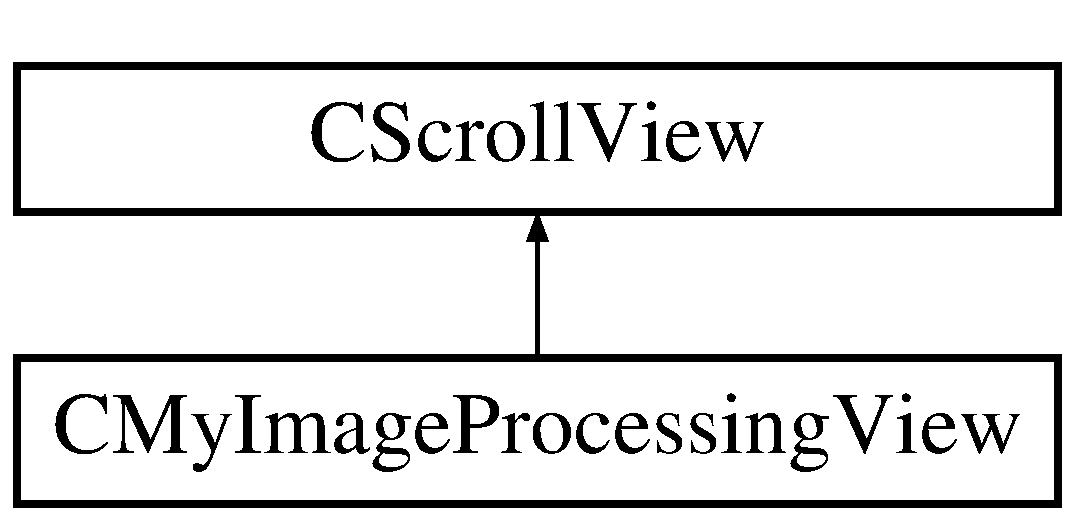
\includegraphics[height=2.000000cm]{class_c_my_image_processing_view}
\end{center}
\end{figure}
\subsection*{Public 멤버 함수}
\begin{DoxyCompactItemize}
\item 
\hyperlink{class_c_my_image_processing_doc}{C\-My\-Image\-Processing\-Doc} $\ast$ \hyperlink{class_c_my_image_processing_view_ae19eb5b26c93701a159e2ba4f8450642}{Get\-Document} () const 
\item 
virtual void \hyperlink{class_c_my_image_processing_view_a8141402da8677e04e9e50643e01cf0dc}{On\-Draw} (C\-D\-C $\ast$p\-D\-C)
\item 
virtual B\-O\-O\-L \hyperlink{class_c_my_image_processing_view_a6fc6c61da49421369f2705b5db7a3008}{Pre\-Create\-Window} (C\-R\-E\-A\-T\-E\-S\-T\-R\-U\-C\-T \&cs)
\item 
virtual \hyperlink{class_c_my_image_processing_view_a62b5e3b81a2aa694615f507e4100c75e}{$\sim$\-C\-My\-Image\-Processing\-View} ()
\item 
afx\-\_\-msg B\-O\-O\-L \hyperlink{class_c_my_image_processing_view_affb65d870bf1d6cd682178ecf64ccab3}{On\-Erase\-Bkgnd} (C\-D\-C $\ast$p\-D\-C)
\end{DoxyCompactItemize}
\subsection*{Protected 멤버 함수}
\begin{DoxyCompactItemize}
\item 
\hyperlink{class_c_my_image_processing_view_a0ccc747475b76eb445e997c6dd5d4496}{C\-My\-Image\-Processing\-View} ()
\item 
virtual void \hyperlink{class_c_my_image_processing_view_aea4e6524b1eb6e73f1f444c1984323af}{On\-Initial\-Update} ()
\end{DoxyCompactItemize}


\subsection{생성자 \& 소멸자 문서화}
\hypertarget{class_c_my_image_processing_view_a0ccc747475b76eb445e997c6dd5d4496}{\index{C\-My\-Image\-Processing\-View@{C\-My\-Image\-Processing\-View}!C\-My\-Image\-Processing\-View@{C\-My\-Image\-Processing\-View}}
\index{C\-My\-Image\-Processing\-View@{C\-My\-Image\-Processing\-View}!CMyImageProcessingView@{C\-My\-Image\-Processing\-View}}
\subsubsection[{C\-My\-Image\-Processing\-View}]{\setlength{\rightskip}{0pt plus 5cm}C\-My\-Image\-Processing\-View\-::\-C\-My\-Image\-Processing\-View (
\begin{DoxyParamCaption}
{}
\end{DoxyParamCaption}
)\hspace{0.3cm}{\ttfamily [protected]}}}\label{class_c_my_image_processing_view_a0ccc747475b76eb445e997c6dd5d4496}
\hypertarget{class_c_my_image_processing_view_a62b5e3b81a2aa694615f507e4100c75e}{\index{C\-My\-Image\-Processing\-View@{C\-My\-Image\-Processing\-View}!$\sim$\-C\-My\-Image\-Processing\-View@{$\sim$\-C\-My\-Image\-Processing\-View}}
\index{$\sim$\-C\-My\-Image\-Processing\-View@{$\sim$\-C\-My\-Image\-Processing\-View}!CMyImageProcessingView@{C\-My\-Image\-Processing\-View}}
\subsubsection[{$\sim$\-C\-My\-Image\-Processing\-View}]{\setlength{\rightskip}{0pt plus 5cm}C\-My\-Image\-Processing\-View\-::$\sim$\-C\-My\-Image\-Processing\-View (
\begin{DoxyParamCaption}
{}
\end{DoxyParamCaption}
)\hspace{0.3cm}{\ttfamily [virtual]}}}\label{class_c_my_image_processing_view_a62b5e3b81a2aa694615f507e4100c75e}


\subsection{멤버 함수 문서화}
\hypertarget{class_c_my_image_processing_view_ae19eb5b26c93701a159e2ba4f8450642}{\index{C\-My\-Image\-Processing\-View@{C\-My\-Image\-Processing\-View}!Get\-Document@{Get\-Document}}
\index{Get\-Document@{Get\-Document}!CMyImageProcessingView@{C\-My\-Image\-Processing\-View}}
\subsubsection[{Get\-Document}]{\setlength{\rightskip}{0pt plus 5cm}{\bf C\-My\-Image\-Processing\-Doc} $\ast$ C\-My\-Image\-Processing\-View\-::\-Get\-Document (
\begin{DoxyParamCaption}
{}
\end{DoxyParamCaption}
) const\hspace{0.3cm}{\ttfamily [inline]}}}\label{class_c_my_image_processing_view_ae19eb5b26c93701a159e2ba4f8450642}
\hypertarget{class_c_my_image_processing_view_a8141402da8677e04e9e50643e01cf0dc}{\index{C\-My\-Image\-Processing\-View@{C\-My\-Image\-Processing\-View}!On\-Draw@{On\-Draw}}
\index{On\-Draw@{On\-Draw}!CMyImageProcessingView@{C\-My\-Image\-Processing\-View}}
\subsubsection[{On\-Draw}]{\setlength{\rightskip}{0pt plus 5cm}void C\-My\-Image\-Processing\-View\-::\-On\-Draw (
\begin{DoxyParamCaption}
\item[{C\-D\-C $\ast$}]{p\-D\-C}
\end{DoxyParamCaption}
)\hspace{0.3cm}{\ttfamily [virtual]}}}\label{class_c_my_image_processing_view_a8141402da8677e04e9e50643e01cf0dc}
\hypertarget{class_c_my_image_processing_view_affb65d870bf1d6cd682178ecf64ccab3}{\index{C\-My\-Image\-Processing\-View@{C\-My\-Image\-Processing\-View}!On\-Erase\-Bkgnd@{On\-Erase\-Bkgnd}}
\index{On\-Erase\-Bkgnd@{On\-Erase\-Bkgnd}!CMyImageProcessingView@{C\-My\-Image\-Processing\-View}}
\subsubsection[{On\-Erase\-Bkgnd}]{\setlength{\rightskip}{0pt plus 5cm}B\-O\-O\-L C\-My\-Image\-Processing\-View\-::\-On\-Erase\-Bkgnd (
\begin{DoxyParamCaption}
\item[{C\-D\-C $\ast$}]{p\-D\-C}
\end{DoxyParamCaption}
)}}\label{class_c_my_image_processing_view_affb65d870bf1d6cd682178ecf64ccab3}
\hypertarget{class_c_my_image_processing_view_aea4e6524b1eb6e73f1f444c1984323af}{\index{C\-My\-Image\-Processing\-View@{C\-My\-Image\-Processing\-View}!On\-Initial\-Update@{On\-Initial\-Update}}
\index{On\-Initial\-Update@{On\-Initial\-Update}!CMyImageProcessingView@{C\-My\-Image\-Processing\-View}}
\subsubsection[{On\-Initial\-Update}]{\setlength{\rightskip}{0pt plus 5cm}void C\-My\-Image\-Processing\-View\-::\-On\-Initial\-Update (
\begin{DoxyParamCaption}
{}
\end{DoxyParamCaption}
)\hspace{0.3cm}{\ttfamily [protected]}, {\ttfamily [virtual]}}}\label{class_c_my_image_processing_view_aea4e6524b1eb6e73f1f444c1984323af}
\hypertarget{class_c_my_image_processing_view_a6fc6c61da49421369f2705b5db7a3008}{\index{C\-My\-Image\-Processing\-View@{C\-My\-Image\-Processing\-View}!Pre\-Create\-Window@{Pre\-Create\-Window}}
\index{Pre\-Create\-Window@{Pre\-Create\-Window}!CMyImageProcessingView@{C\-My\-Image\-Processing\-View}}
\subsubsection[{Pre\-Create\-Window}]{\setlength{\rightskip}{0pt plus 5cm}B\-O\-O\-L C\-My\-Image\-Processing\-View\-::\-Pre\-Create\-Window (
\begin{DoxyParamCaption}
\item[{C\-R\-E\-A\-T\-E\-S\-T\-R\-U\-C\-T \&}]{cs}
\end{DoxyParamCaption}
)\hspace{0.3cm}{\ttfamily [virtual]}}}\label{class_c_my_image_processing_view_a6fc6c61da49421369f2705b5db7a3008}


이 클래스에 대한 문서화 페이지는 다음의 파일들로부터 생성되었습니다.\-:\begin{DoxyCompactItemize}
\item 
H\-:/\-Repository/\-My\-Image\-Processing/\-My\-Image\-Processing/\hyperlink{_my_image_processing_view_8h}{My\-Image\-Processing\-View.\-h}\item 
H\-:/\-Repository/\-My\-Image\-Processing/\-My\-Image\-Processing/\hyperlink{_my_image_processing_view_8cpp}{My\-Image\-Processing\-View.\-cpp}\end{DoxyCompactItemize}

\hypertarget{class_c_pow_dlg}{\section{C\-Pow\-Dlg 클래스 참조}
\label{class_c_pow_dlg}\index{C\-Pow\-Dlg@{C\-Pow\-Dlg}}
}


{\ttfamily \#include $<$Pow\-Dlg.\-h$>$}

C\-Pow\-Dlg에 대한 상속 다이어그램 \-: \begin{figure}[H]
\begin{center}
\leavevmode
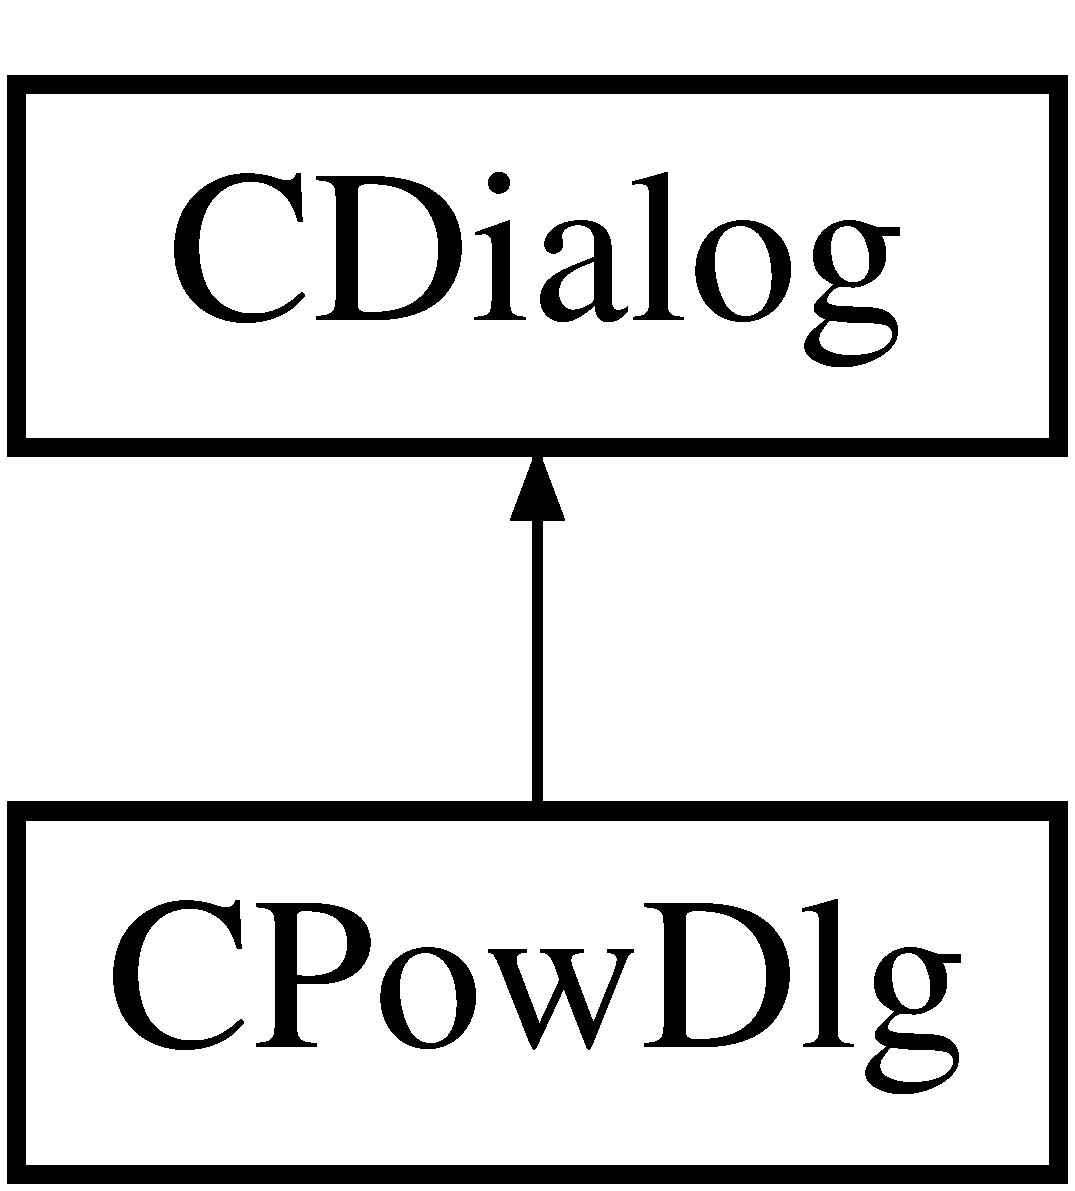
\includegraphics[height=2.000000cm]{class_c_pow_dlg}
\end{center}
\end{figure}
\subsection*{Public 타입}
\begin{DoxyCompactItemize}
\item 
enum \{ \hyperlink{class_c_pow_dlg_a683a28f8cb6129b2d9f1a8b992832120ac1b1f511a60bab7cfaa28eba3c6a15e5}{I\-D\-D} = I\-D\-D\-\_\-\-P\-O\-W\-\_\-\-D\-L\-G
 \}
\end{DoxyCompactItemize}
\subsection*{Public 멤버 함수}
\begin{DoxyCompactItemize}
\item 
\hyperlink{class_c_pow_dlg_ae9a905bda1e55e4ca19b1a47032f74a4}{C\-Pow\-Dlg} (C\-Wnd $\ast$p\-Parent=N\-U\-L\-L)
\item 
virtual \hyperlink{class_c_pow_dlg_adfea03ae30c4fe603b1e8f762f5d1753}{$\sim$\-C\-Pow\-Dlg} ()
\end{DoxyCompactItemize}
\subsection*{Public 속성}
\begin{DoxyCompactItemize}
\item 
double \hyperlink{class_c_pow_dlg_a62c895a66edd34c933bbe99371ca1ecf}{m\-\_\-t}
\end{DoxyCompactItemize}
\subsection*{Protected 멤버 함수}
\begin{DoxyCompactItemize}
\item 
virtual void \hyperlink{class_c_pow_dlg_ae14602a28d4e977498508f5c6212bc57}{Do\-Data\-Exchange} (C\-Data\-Exchange $\ast$p\-D\-X)
\end{DoxyCompactItemize}


\subsection{멤버 열거형 문서화}
\hypertarget{class_c_pow_dlg_a683a28f8cb6129b2d9f1a8b992832120}{\subsubsection[{anonymous enum}]{\setlength{\rightskip}{0pt plus 5cm}anonymous enum}}\label{class_c_pow_dlg_a683a28f8cb6129b2d9f1a8b992832120}
\begin{Desc}
\item[열거형 멤버\-: ]\par
\begin{description}
\index{I\-D\-D@{I\-D\-D}!C\-Pow\-Dlg@{C\-Pow\-Dlg}}\index{C\-Pow\-Dlg@{C\-Pow\-Dlg}!I\-D\-D@{I\-D\-D}}\item[{\em 
\hypertarget{class_c_pow_dlg_a683a28f8cb6129b2d9f1a8b992832120ac1b1f511a60bab7cfaa28eba3c6a15e5}{I\-D\-D}\label{class_c_pow_dlg_a683a28f8cb6129b2d9f1a8b992832120ac1b1f511a60bab7cfaa28eba3c6a15e5}
}]\end{description}
\end{Desc}



\subsection{생성자 \& 소멸자 문서화}
\hypertarget{class_c_pow_dlg_ae9a905bda1e55e4ca19b1a47032f74a4}{\index{C\-Pow\-Dlg@{C\-Pow\-Dlg}!C\-Pow\-Dlg@{C\-Pow\-Dlg}}
\index{C\-Pow\-Dlg@{C\-Pow\-Dlg}!CPowDlg@{C\-Pow\-Dlg}}
\subsubsection[{C\-Pow\-Dlg}]{\setlength{\rightskip}{0pt plus 5cm}C\-Pow\-Dlg\-::\-C\-Pow\-Dlg (
\begin{DoxyParamCaption}
\item[{C\-Wnd $\ast$}]{p\-Parent = {\ttfamily NULL}}
\end{DoxyParamCaption}
)}}\label{class_c_pow_dlg_ae9a905bda1e55e4ca19b1a47032f74a4}
\hypertarget{class_c_pow_dlg_adfea03ae30c4fe603b1e8f762f5d1753}{\index{C\-Pow\-Dlg@{C\-Pow\-Dlg}!$\sim$\-C\-Pow\-Dlg@{$\sim$\-C\-Pow\-Dlg}}
\index{$\sim$\-C\-Pow\-Dlg@{$\sim$\-C\-Pow\-Dlg}!CPowDlg@{C\-Pow\-Dlg}}
\subsubsection[{$\sim$\-C\-Pow\-Dlg}]{\setlength{\rightskip}{0pt plus 5cm}C\-Pow\-Dlg\-::$\sim$\-C\-Pow\-Dlg (
\begin{DoxyParamCaption}
{}
\end{DoxyParamCaption}
)\hspace{0.3cm}{\ttfamily [virtual]}}}\label{class_c_pow_dlg_adfea03ae30c4fe603b1e8f762f5d1753}


\subsection{멤버 함수 문서화}
\hypertarget{class_c_pow_dlg_ae14602a28d4e977498508f5c6212bc57}{\index{C\-Pow\-Dlg@{C\-Pow\-Dlg}!Do\-Data\-Exchange@{Do\-Data\-Exchange}}
\index{Do\-Data\-Exchange@{Do\-Data\-Exchange}!CPowDlg@{C\-Pow\-Dlg}}
\subsubsection[{Do\-Data\-Exchange}]{\setlength{\rightskip}{0pt plus 5cm}void C\-Pow\-Dlg\-::\-Do\-Data\-Exchange (
\begin{DoxyParamCaption}
\item[{C\-Data\-Exchange $\ast$}]{p\-D\-X}
\end{DoxyParamCaption}
)\hspace{0.3cm}{\ttfamily [protected]}, {\ttfamily [virtual]}}}\label{class_c_pow_dlg_ae14602a28d4e977498508f5c6212bc57}


\subsection{멤버 데이타 문서화}
\hypertarget{class_c_pow_dlg_a62c895a66edd34c933bbe99371ca1ecf}{\index{C\-Pow\-Dlg@{C\-Pow\-Dlg}!m\-\_\-t@{m\-\_\-t}}
\index{m\-\_\-t@{m\-\_\-t}!CPowDlg@{C\-Pow\-Dlg}}
\subsubsection[{m\-\_\-t}]{\setlength{\rightskip}{0pt plus 5cm}double C\-Pow\-Dlg\-::m\-\_\-t}}\label{class_c_pow_dlg_a62c895a66edd34c933bbe99371ca1ecf}


이 클래스에 대한 문서화 페이지는 다음의 파일들로부터 생성되었습니다.\-:\begin{DoxyCompactItemize}
\item 
My\-Image\-Processing/\hyperlink{_pow_dlg_8h}{Pow\-Dlg.\-h}\item 
My\-Image\-Processing/\hyperlink{_pow_dlg_8cpp}{Pow\-Dlg.\-cpp}\end{DoxyCompactItemize}

\hypertarget{class_c_scl_dlg}{\section{C\-Scl\-Dlg 클래스 참조}
\label{class_c_scl_dlg}\index{C\-Scl\-Dlg@{C\-Scl\-Dlg}}
}


{\ttfamily \#include $<$Scl\-Dlg.\-h$>$}

C\-Scl\-Dlg에 대한 상속 다이어그램 \-: \begin{figure}[H]
\begin{center}
\leavevmode
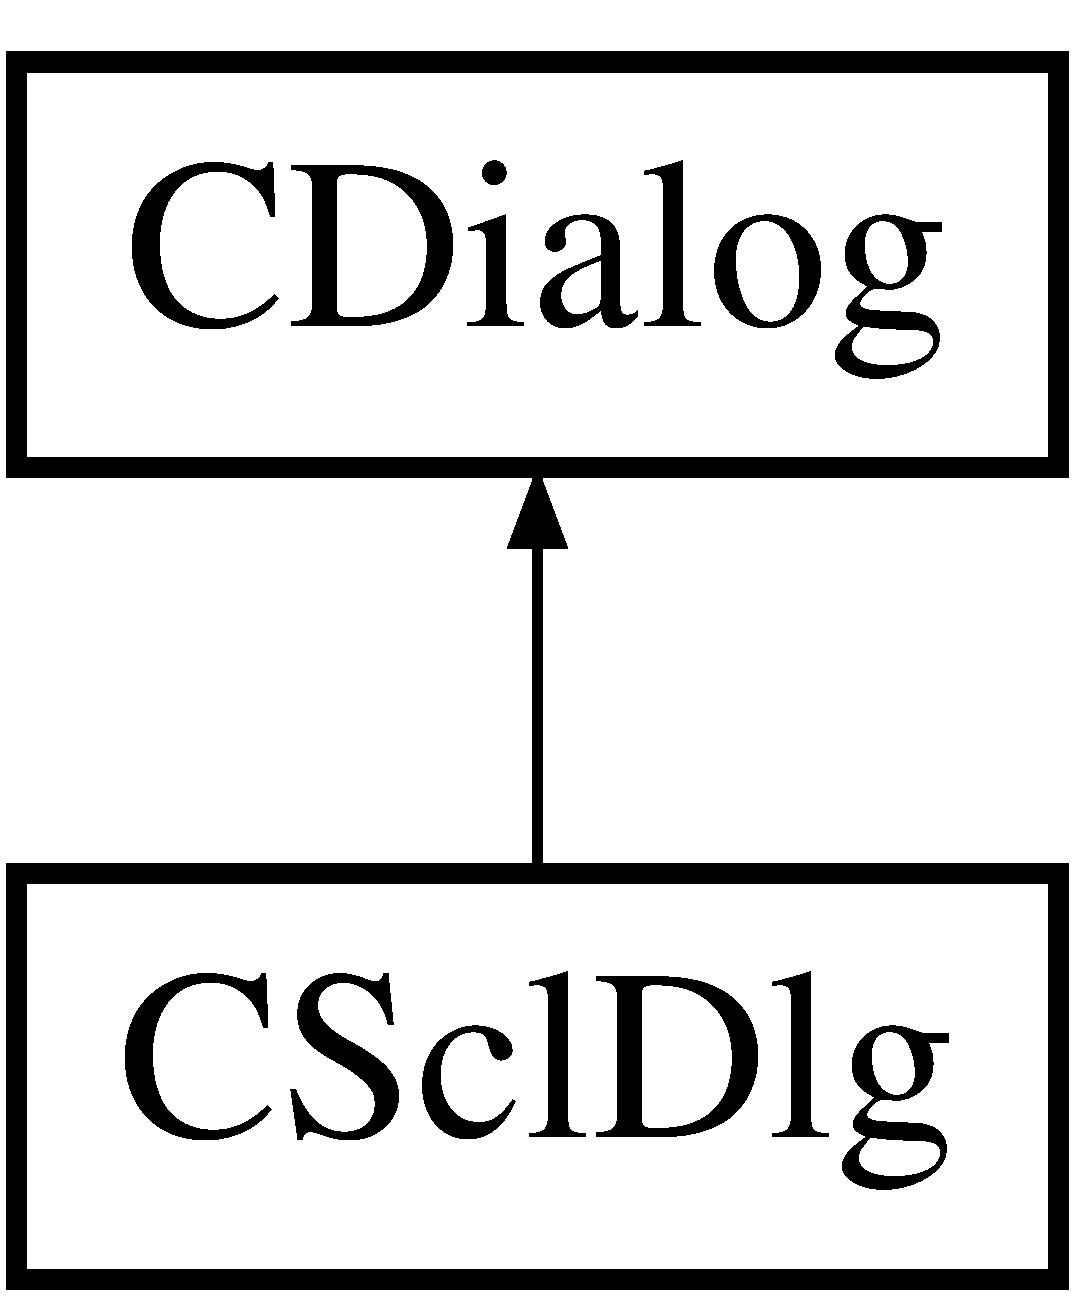
\includegraphics[height=2.000000cm]{class_c_scl_dlg}
\end{center}
\end{figure}
\subsection*{Public 타입}
\begin{DoxyCompactItemize}
\item 
enum \{ \hyperlink{class_c_scl_dlg_a1ed7185c27a2ce41c94d772b6b1bd6eca37c13cd75af0df4b69cff990e78b8c5c}{I\-D\-D} = I\-D\-D\-\_\-\-D\-I\-A\-L\-O\-G1
 \}
\end{DoxyCompactItemize}
\subsection*{Public 멤버 함수}
\begin{DoxyCompactItemize}
\item 
\hyperlink{class_c_scl_dlg_a0024f026091f91c0850e77b103f5f30a}{C\-Scl\-Dlg} (C\-Wnd $\ast$p\-Parent=N\-U\-L\-L)
\item 
virtual \hyperlink{class_c_scl_dlg_a643c698da9bdf5e630a9c452812b0db5}{$\sim$\-C\-Scl\-Dlg} ()
\end{DoxyCompactItemize}
\subsection*{Public 속성}
\begin{DoxyCompactItemize}
\item 
int \hyperlink{class_c_scl_dlg_aa52708335531c455850915172bff26ba}{m\-\_\-n\-Type}
\item 
int \hyperlink{class_c_scl_dlg_ae24bfb6ef6de4cb6cbc6f3b6cdae619b}{m\-\_\-\-Cx}
\item 
int \hyperlink{class_c_scl_dlg_a6864c7ad7a17b92a9c9e670a871cf9d9}{m\-\_\-\-Cy}
\end{DoxyCompactItemize}
\subsection*{Protected 멤버 함수}
\begin{DoxyCompactItemize}
\item 
virtual void \hyperlink{class_c_scl_dlg_ac310ef75be8baafc95824aed2cc6ba23}{Do\-Data\-Exchange} (C\-Data\-Exchange $\ast$p\-D\-X)
\end{DoxyCompactItemize}


\subsection{멤버 열거형 문서화}
\hypertarget{class_c_scl_dlg_a1ed7185c27a2ce41c94d772b6b1bd6ec}{\subsubsection[{anonymous enum}]{\setlength{\rightskip}{0pt plus 5cm}anonymous enum}}\label{class_c_scl_dlg_a1ed7185c27a2ce41c94d772b6b1bd6ec}
\begin{Desc}
\item[열거형 멤버\-: ]\par
\begin{description}
\index{I\-D\-D@{I\-D\-D}!C\-Scl\-Dlg@{C\-Scl\-Dlg}}\index{C\-Scl\-Dlg@{C\-Scl\-Dlg}!I\-D\-D@{I\-D\-D}}\item[{\em 
\hypertarget{class_c_scl_dlg_a1ed7185c27a2ce41c94d772b6b1bd6eca37c13cd75af0df4b69cff990e78b8c5c}{I\-D\-D}\label{class_c_scl_dlg_a1ed7185c27a2ce41c94d772b6b1bd6eca37c13cd75af0df4b69cff990e78b8c5c}
}]\end{description}
\end{Desc}



\subsection{생성자 \& 소멸자 문서화}
\hypertarget{class_c_scl_dlg_a0024f026091f91c0850e77b103f5f30a}{\index{C\-Scl\-Dlg@{C\-Scl\-Dlg}!C\-Scl\-Dlg@{C\-Scl\-Dlg}}
\index{C\-Scl\-Dlg@{C\-Scl\-Dlg}!CSclDlg@{C\-Scl\-Dlg}}
\subsubsection[{C\-Scl\-Dlg}]{\setlength{\rightskip}{0pt plus 5cm}C\-Scl\-Dlg\-::\-C\-Scl\-Dlg (
\begin{DoxyParamCaption}
\item[{C\-Wnd $\ast$}]{p\-Parent = {\ttfamily NULL}}
\end{DoxyParamCaption}
)}}\label{class_c_scl_dlg_a0024f026091f91c0850e77b103f5f30a}
\hypertarget{class_c_scl_dlg_a643c698da9bdf5e630a9c452812b0db5}{\index{C\-Scl\-Dlg@{C\-Scl\-Dlg}!$\sim$\-C\-Scl\-Dlg@{$\sim$\-C\-Scl\-Dlg}}
\index{$\sim$\-C\-Scl\-Dlg@{$\sim$\-C\-Scl\-Dlg}!CSclDlg@{C\-Scl\-Dlg}}
\subsubsection[{$\sim$\-C\-Scl\-Dlg}]{\setlength{\rightskip}{0pt plus 5cm}C\-Scl\-Dlg\-::$\sim$\-C\-Scl\-Dlg (
\begin{DoxyParamCaption}
{}
\end{DoxyParamCaption}
)\hspace{0.3cm}{\ttfamily [virtual]}}}\label{class_c_scl_dlg_a643c698da9bdf5e630a9c452812b0db5}


\subsection{멤버 함수 문서화}
\hypertarget{class_c_scl_dlg_ac310ef75be8baafc95824aed2cc6ba23}{\index{C\-Scl\-Dlg@{C\-Scl\-Dlg}!Do\-Data\-Exchange@{Do\-Data\-Exchange}}
\index{Do\-Data\-Exchange@{Do\-Data\-Exchange}!CSclDlg@{C\-Scl\-Dlg}}
\subsubsection[{Do\-Data\-Exchange}]{\setlength{\rightskip}{0pt plus 5cm}void C\-Scl\-Dlg\-::\-Do\-Data\-Exchange (
\begin{DoxyParamCaption}
\item[{C\-Data\-Exchange $\ast$}]{p\-D\-X}
\end{DoxyParamCaption}
)\hspace{0.3cm}{\ttfamily [protected]}, {\ttfamily [virtual]}}}\label{class_c_scl_dlg_ac310ef75be8baafc95824aed2cc6ba23}


\subsection{멤버 데이타 문서화}
\hypertarget{class_c_scl_dlg_ae24bfb6ef6de4cb6cbc6f3b6cdae619b}{\index{C\-Scl\-Dlg@{C\-Scl\-Dlg}!m\-\_\-\-Cx@{m\-\_\-\-Cx}}
\index{m\-\_\-\-Cx@{m\-\_\-\-Cx}!CSclDlg@{C\-Scl\-Dlg}}
\subsubsection[{m\-\_\-\-Cx}]{\setlength{\rightskip}{0pt plus 5cm}int C\-Scl\-Dlg\-::m\-\_\-\-Cx}}\label{class_c_scl_dlg_ae24bfb6ef6de4cb6cbc6f3b6cdae619b}
\hypertarget{class_c_scl_dlg_a6864c7ad7a17b92a9c9e670a871cf9d9}{\index{C\-Scl\-Dlg@{C\-Scl\-Dlg}!m\-\_\-\-Cy@{m\-\_\-\-Cy}}
\index{m\-\_\-\-Cy@{m\-\_\-\-Cy}!CSclDlg@{C\-Scl\-Dlg}}
\subsubsection[{m\-\_\-\-Cy}]{\setlength{\rightskip}{0pt plus 5cm}int C\-Scl\-Dlg\-::m\-\_\-\-Cy}}\label{class_c_scl_dlg_a6864c7ad7a17b92a9c9e670a871cf9d9}
\hypertarget{class_c_scl_dlg_aa52708335531c455850915172bff26ba}{\index{C\-Scl\-Dlg@{C\-Scl\-Dlg}!m\-\_\-n\-Type@{m\-\_\-n\-Type}}
\index{m\-\_\-n\-Type@{m\-\_\-n\-Type}!CSclDlg@{C\-Scl\-Dlg}}
\subsubsection[{m\-\_\-n\-Type}]{\setlength{\rightskip}{0pt plus 5cm}int C\-Scl\-Dlg\-::m\-\_\-n\-Type}}\label{class_c_scl_dlg_aa52708335531c455850915172bff26ba}


이 클래스에 대한 문서화 페이지는 다음의 파일들로부터 생성되었습니다.\-:\begin{DoxyCompactItemize}
\item 
My\-Image\-Processing/\hyperlink{_scl_dlg_8h}{Scl\-Dlg.\-h}\item 
My\-Image\-Processing/\hyperlink{_scl_dlg_8cpp}{Scl\-Dlg.\-cpp}\end{DoxyCompactItemize}

\hypertarget{class_m_a_t_r_i_x2_d}{\section{M\-A\-T\-R\-I\-X2\-D 클래스 참조}
\label{class_m_a_t_r_i_x2_d}\index{M\-A\-T\-R\-I\-X2\-D@{M\-A\-T\-R\-I\-X2\-D}}
}


{\ttfamily \#include $<$matrix.\-h$>$}

\subsection*{Public 멤버 함수}
\begin{DoxyCompactItemize}
\item 
\hyperlink{class_m_a_t_r_i_x2_d_a34e47a9c3d3006372f43d1f593a253df}{M\-A\-T\-R\-I\-X2\-D} ()
\begin{DoxyCompactList}\small\item\em 2차원 행렬 표현 \end{DoxyCompactList}\item 
\hyperlink{class_m_a_t_r_i_x2_d_a47149410e6e90d06ceb211eec22ee822}{M\-A\-T\-R\-I\-X2\-D} (\hyperlink{class_m_a_t_r_i_x2_d}{M\-A\-T\-R\-I\-X2\-D} \&mat)
\begin{DoxyCompactList}\small\item\em copy constructor \end{DoxyCompactList}\item 
\hyperlink{class_m_a_t_r_i_x2_d_aacd4a6b2603c7d34c08da1ddf118ab19}{M\-A\-T\-R\-I\-X2\-D} (double \hyperlink{class_m_a_t_r_i_x2_d_a4ae1e61f3b886f9b3ce346f6d54de973}{a}\mbox{[}$\,$\mbox{]}\mbox{[}2\mbox{]})
\item 
\hyperlink{class_m_a_t_r_i_x2_d_a5b4703886bd5d30d4bc47fff85488b04}{M\-A\-T\-R\-I\-X2\-D} (double t\mbox{[}$\,$\mbox{]}, int n)
\begin{DoxyCompactList}\small\item\em double형 1차원 배열을 2차원 행렬화 \end{DoxyCompactList}\item 
double \hyperlink{class_m_a_t_r_i_x2_d_a0c4cad4dbb6ad4a5a560d4c9876cd071}{get\-Det} ()
\item 
bool \hyperlink{class_m_a_t_r_i_x2_d_ae5018742fa0dfa84dbb2466c0789bdcd}{is\-Inversible} ()
\begin{DoxyCompactList}\small\item\em Inverse 가능 여부, Det가 0이면 false. \end{DoxyCompactList}\item 
\hyperlink{class_m_a_t_r_i_x2_d}{M\-A\-T\-R\-I\-X2\-D} \hyperlink{class_m_a_t_r_i_x2_d_a8593d4fd11d45ea256047900ebc77307}{inverse} ()
\begin{DoxyCompactList}\small\item\em this의 역행렬을 구해 반환 \end{DoxyCompactList}\end{DoxyCompactItemize}
\subsection*{Private 속성}
\begin{DoxyCompactItemize}
\item 
double \hyperlink{class_m_a_t_r_i_x2_d_a4ae1e61f3b886f9b3ce346f6d54de973}{a} \mbox{[}2\mbox{]}\mbox{[}2\mbox{]}
\begin{DoxyCompactList}\small\item\em 행렬 원소 (2$\ast$2) \end{DoxyCompactList}\end{DoxyCompactItemize}


\subsection{생성자 \& 소멸자 문서화}
\hypertarget{class_m_a_t_r_i_x2_d_a34e47a9c3d3006372f43d1f593a253df}{\index{M\-A\-T\-R\-I\-X2\-D@{M\-A\-T\-R\-I\-X2\-D}!M\-A\-T\-R\-I\-X2\-D@{M\-A\-T\-R\-I\-X2\-D}}
\index{M\-A\-T\-R\-I\-X2\-D@{M\-A\-T\-R\-I\-X2\-D}!MATRIX2D@{M\-A\-T\-R\-I\-X2\-D}}
\subsubsection[{M\-A\-T\-R\-I\-X2\-D}]{\setlength{\rightskip}{0pt plus 5cm}M\-A\-T\-R\-I\-X2\-D\-::\-M\-A\-T\-R\-I\-X2\-D (
\begin{DoxyParamCaption}
{}
\end{DoxyParamCaption}
)\hspace{0.3cm}{\ttfamily [inline]}}}\label{class_m_a_t_r_i_x2_d_a34e47a9c3d3006372f43d1f593a253df}


2차원 행렬 표현 

\hypertarget{class_m_a_t_r_i_x2_d_a47149410e6e90d06ceb211eec22ee822}{\index{M\-A\-T\-R\-I\-X2\-D@{M\-A\-T\-R\-I\-X2\-D}!M\-A\-T\-R\-I\-X2\-D@{M\-A\-T\-R\-I\-X2\-D}}
\index{M\-A\-T\-R\-I\-X2\-D@{M\-A\-T\-R\-I\-X2\-D}!MATRIX2D@{M\-A\-T\-R\-I\-X2\-D}}
\subsubsection[{M\-A\-T\-R\-I\-X2\-D}]{\setlength{\rightskip}{0pt plus 5cm}M\-A\-T\-R\-I\-X2\-D\-::\-M\-A\-T\-R\-I\-X2\-D (
\begin{DoxyParamCaption}
\item[{{\bf M\-A\-T\-R\-I\-X2\-D} \&}]{mat}
\end{DoxyParamCaption}
)\hspace{0.3cm}{\ttfamily [inline]}}}\label{class_m_a_t_r_i_x2_d_a47149410e6e90d06ceb211eec22ee822}


copy constructor 

\hypertarget{class_m_a_t_r_i_x2_d_aacd4a6b2603c7d34c08da1ddf118ab19}{\index{M\-A\-T\-R\-I\-X2\-D@{M\-A\-T\-R\-I\-X2\-D}!M\-A\-T\-R\-I\-X2\-D@{M\-A\-T\-R\-I\-X2\-D}}
\index{M\-A\-T\-R\-I\-X2\-D@{M\-A\-T\-R\-I\-X2\-D}!MATRIX2D@{M\-A\-T\-R\-I\-X2\-D}}
\subsubsection[{M\-A\-T\-R\-I\-X2\-D}]{\setlength{\rightskip}{0pt plus 5cm}M\-A\-T\-R\-I\-X2\-D\-::\-M\-A\-T\-R\-I\-X2\-D (
\begin{DoxyParamCaption}
\item[{double}]{a\mbox{[}$\,$\mbox{]}\mbox{[}2\mbox{]}}
\end{DoxyParamCaption}
)\hspace{0.3cm}{\ttfamily [inline]}}}\label{class_m_a_t_r_i_x2_d_aacd4a6b2603c7d34c08da1ddf118ab19}
double형 2차원 배열을 행렬화 
\begin{DoxyParams}{매개변수}
{\em a} & \-: 2차원 배열 (2 $\ast$ 2) \\
\hline
\end{DoxyParams}
\hypertarget{class_m_a_t_r_i_x2_d_a5b4703886bd5d30d4bc47fff85488b04}{\index{M\-A\-T\-R\-I\-X2\-D@{M\-A\-T\-R\-I\-X2\-D}!M\-A\-T\-R\-I\-X2\-D@{M\-A\-T\-R\-I\-X2\-D}}
\index{M\-A\-T\-R\-I\-X2\-D@{M\-A\-T\-R\-I\-X2\-D}!MATRIX2D@{M\-A\-T\-R\-I\-X2\-D}}
\subsubsection[{M\-A\-T\-R\-I\-X2\-D}]{\setlength{\rightskip}{0pt plus 5cm}M\-A\-T\-R\-I\-X2\-D\-::\-M\-A\-T\-R\-I\-X2\-D (
\begin{DoxyParamCaption}
\item[{double}]{t\mbox{[}$\,$\mbox{]}, }
\item[{int}]{n}
\end{DoxyParamCaption}
)\hspace{0.3cm}{\ttfamily [inline]}}}\label{class_m_a_t_r_i_x2_d_a5b4703886bd5d30d4bc47fff85488b04}


double형 1차원 배열을 2차원 행렬화 


\begin{DoxyParams}{매개변수}
{\em t} & \-: 1차원 배열 (1 $\ast$ 4) \\
\hline
{\em n} & \-: 크기(must be 4) \\
\hline
\end{DoxyParams}


\subsection{멤버 함수 문서화}
\hypertarget{class_m_a_t_r_i_x2_d_a0c4cad4dbb6ad4a5a560d4c9876cd071}{\index{M\-A\-T\-R\-I\-X2\-D@{M\-A\-T\-R\-I\-X2\-D}!get\-Det@{get\-Det}}
\index{get\-Det@{get\-Det}!MATRIX2D@{M\-A\-T\-R\-I\-X2\-D}}
\subsubsection[{get\-Det}]{\setlength{\rightskip}{0pt plus 5cm}double M\-A\-T\-R\-I\-X2\-D\-::get\-Det (
\begin{DoxyParamCaption}
{}
\end{DoxyParamCaption}
)\hspace{0.3cm}{\ttfamily [inline]}}}\label{class_m_a_t_r_i_x2_d_a0c4cad4dbb6ad4a5a560d4c9876cd071}
get Determinant \hypertarget{class_m_a_t_r_i_x2_d_a8593d4fd11d45ea256047900ebc77307}{\index{M\-A\-T\-R\-I\-X2\-D@{M\-A\-T\-R\-I\-X2\-D}!inverse@{inverse}}
\index{inverse@{inverse}!MATRIX2D@{M\-A\-T\-R\-I\-X2\-D}}
\subsubsection[{inverse}]{\setlength{\rightskip}{0pt plus 5cm}{\bf M\-A\-T\-R\-I\-X2\-D} M\-A\-T\-R\-I\-X2\-D\-::inverse (
\begin{DoxyParamCaption}
{}
\end{DoxyParamCaption}
)\hspace{0.3cm}{\ttfamily [inline]}}}\label{class_m_a_t_r_i_x2_d_a8593d4fd11d45ea256047900ebc77307}


this의 역행렬을 구해 반환 

\hypertarget{class_m_a_t_r_i_x2_d_ae5018742fa0dfa84dbb2466c0789bdcd}{\index{M\-A\-T\-R\-I\-X2\-D@{M\-A\-T\-R\-I\-X2\-D}!is\-Inversible@{is\-Inversible}}
\index{is\-Inversible@{is\-Inversible}!MATRIX2D@{M\-A\-T\-R\-I\-X2\-D}}
\subsubsection[{is\-Inversible}]{\setlength{\rightskip}{0pt plus 5cm}bool M\-A\-T\-R\-I\-X2\-D\-::is\-Inversible (
\begin{DoxyParamCaption}
{}
\end{DoxyParamCaption}
)\hspace{0.3cm}{\ttfamily [inline]}}}\label{class_m_a_t_r_i_x2_d_ae5018742fa0dfa84dbb2466c0789bdcd}


Inverse 가능 여부, Det가 0이면 false. 



\subsection{멤버 데이타 문서화}
\hypertarget{class_m_a_t_r_i_x2_d_a4ae1e61f3b886f9b3ce346f6d54de973}{\index{M\-A\-T\-R\-I\-X2\-D@{M\-A\-T\-R\-I\-X2\-D}!a@{a}}
\index{a@{a}!MATRIX2D@{M\-A\-T\-R\-I\-X2\-D}}
\subsubsection[{a}]{\setlength{\rightskip}{0pt plus 5cm}double M\-A\-T\-R\-I\-X2\-D\-::a\mbox{[}2\mbox{]}\mbox{[}2\mbox{]}\hspace{0.3cm}{\ttfamily [private]}}}\label{class_m_a_t_r_i_x2_d_a4ae1e61f3b886f9b3ce346f6d54de973}


행렬 원소 (2$\ast$2) 



이 클래스에 대한 문서화 페이지는 다음의 파일로부터 생성되었습니다.\-:\begin{DoxyCompactItemize}
\item 
H\-:/\-Repository/\-My\-Image\-Processing/\-My\-Image\-Processing/\hyperlink{matrix_8h}{matrix.\-h}\end{DoxyCompactItemize}

\hypertarget{class_m_a_t_r_i_x3_d}{\section{M\-A\-T\-R\-I\-X3\-D 클래스 참조}
\label{class_m_a_t_r_i_x3_d}\index{M\-A\-T\-R\-I\-X3\-D@{M\-A\-T\-R\-I\-X3\-D}}
}


{\ttfamily \#include $<$matrix.\-h$>$}

\subsection*{Public 멤버 함수}
\begin{DoxyCompactItemize}
\item 
\hyperlink{class_m_a_t_r_i_x3_d_a85e81a995201846d602ab80f502626e6}{M\-A\-T\-R\-I\-X3\-D} ()
\begin{DoxyCompactList}\small\item\em 3차원 행렬 표현 \end{DoxyCompactList}\item 
\hyperlink{class_m_a_t_r_i_x3_d_a464aa49f42a93b7ec7af34cad6db379f}{M\-A\-T\-R\-I\-X3\-D} (\hyperlink{class_m_a_t_r_i_x3_d}{M\-A\-T\-R\-I\-X3\-D} \&mat)
\begin{DoxyCompactList}\small\item\em copy constructor, calculate determinant in advance. \end{DoxyCompactList}\item 
\hyperlink{class_m_a_t_r_i_x3_d_a767e7bb59466d96793b89a7f2db0a1a4}{M\-A\-T\-R\-I\-X3\-D} (double a\mbox{[}$\,$\mbox{]}\mbox{[}3\mbox{]})
\item 
bool \hyperlink{class_m_a_t_r_i_x3_d_ae04bbddf00d6572e12b67eb9a0d6d55f}{is\-Inversible} ()
\begin{DoxyCompactList}\small\item\em Inverse 가능 여부, Det가 0이면 false. \end{DoxyCompactList}\item 
double \hyperlink{class_m_a_t_r_i_x3_d_ab9708baa5af2ffe980632870e88c1559}{get\-Det} ()
\item 
double \hyperlink{class_m_a_t_r_i_x3_d_a23292251c50eab390168914069cefc0e}{get\-Cofactor} (int \-\_\-i, int \-\_\-j)
\item 
void \hyperlink{class_m_a_t_r_i_x3_d_ac3e4b69526d21abcc0db1ddd1718b6a8}{set} (int i, int j, double v)
\item 
double \hyperlink{class_m_a_t_r_i_x3_d_a215a4ab44606797cd7f2b1551cd05431}{get} (int i, int j)
\item 
\hyperlink{class_m_a_t_r_i_x3_d}{M\-A\-T\-R\-I\-X3\-D} \hyperlink{class_m_a_t_r_i_x3_d_a4133adf628205e22c49d420d80f4336e}{inverse} ()
\item 
\hyperlink{class___p_o_i_n_t}{\-\_\-\-P\-O\-I\-N\-T} \hyperlink{class_m_a_t_r_i_x3_d_a9c5556589092317bb63fbb8b681035ab}{Affine\-Transform} (\hyperlink{class___p_o_i_n_t}{\-\_\-\-P\-O\-I\-N\-T} \&input)
\end{DoxyCompactItemize}
\subsection*{Private 멤버 함수}
\begin{DoxyCompactItemize}
\item 
double \hyperlink{class_m_a_t_r_i_x3_d_a81930ff56a1e199b2d3e606f27ed0a29}{calc\-Det} ()
\begin{DoxyCompactList}\small\item\em 판별식을 계산하기 위한 함수 \end{DoxyCompactList}\end{DoxyCompactItemize}
\subsection*{Private 속성}
\begin{DoxyCompactItemize}
\item 
bool \hyperlink{class_m_a_t_r_i_x3_d_ab951cbc695222c9cd96d1f2990b1a662}{det\-\_\-flag}
\begin{DoxyCompactList}\small\item\em Determinant 계산 여부, 미리 계산하기 위함 \end{DoxyCompactList}\item 
bool \hyperlink{class_m_a_t_r_i_x3_d_a3d3bd9c2ee0c213ca2f69804c3db6ac6}{is\-Set}
\begin{DoxyCompactList}\small\item\em 행렬의 값이 설정되었는지 여부 \end{DoxyCompactList}\item 
double \hyperlink{class_m_a_t_r_i_x3_d_ad46f057c72ed680b5d94f7b168908fc9}{A} \mbox{[}3\mbox{]}\mbox{[}3\mbox{]}
\begin{DoxyCompactList}\small\item\em 실제 행렬 값 \end{DoxyCompactList}\item 
double \hyperlink{class_m_a_t_r_i_x3_d_a836b104900b7c16a92bda6e41612a77d}{det}
\begin{DoxyCompactList}\small\item\em Determinant. \end{DoxyCompactList}\end{DoxyCompactItemize}


\subsection{생성자 \& 소멸자 문서화}
\hypertarget{class_m_a_t_r_i_x3_d_a85e81a995201846d602ab80f502626e6}{\index{M\-A\-T\-R\-I\-X3\-D@{M\-A\-T\-R\-I\-X3\-D}!M\-A\-T\-R\-I\-X3\-D@{M\-A\-T\-R\-I\-X3\-D}}
\index{M\-A\-T\-R\-I\-X3\-D@{M\-A\-T\-R\-I\-X3\-D}!MATRIX3D@{M\-A\-T\-R\-I\-X3\-D}}
\subsubsection[{M\-A\-T\-R\-I\-X3\-D}]{\setlength{\rightskip}{0pt plus 5cm}M\-A\-T\-R\-I\-X3\-D\-::\-M\-A\-T\-R\-I\-X3\-D (
\begin{DoxyParamCaption}
{}
\end{DoxyParamCaption}
)\hspace{0.3cm}{\ttfamily [inline]}}}\label{class_m_a_t_r_i_x3_d_a85e81a995201846d602ab80f502626e6}


3차원 행렬 표현 

\hypertarget{class_m_a_t_r_i_x3_d_a464aa49f42a93b7ec7af34cad6db379f}{\index{M\-A\-T\-R\-I\-X3\-D@{M\-A\-T\-R\-I\-X3\-D}!M\-A\-T\-R\-I\-X3\-D@{M\-A\-T\-R\-I\-X3\-D}}
\index{M\-A\-T\-R\-I\-X3\-D@{M\-A\-T\-R\-I\-X3\-D}!MATRIX3D@{M\-A\-T\-R\-I\-X3\-D}}
\subsubsection[{M\-A\-T\-R\-I\-X3\-D}]{\setlength{\rightskip}{0pt plus 5cm}M\-A\-T\-R\-I\-X3\-D\-::\-M\-A\-T\-R\-I\-X3\-D (
\begin{DoxyParamCaption}
\item[{{\bf M\-A\-T\-R\-I\-X3\-D} \&}]{mat}
\end{DoxyParamCaption}
)\hspace{0.3cm}{\ttfamily [inline]}}}\label{class_m_a_t_r_i_x3_d_a464aa49f42a93b7ec7af34cad6db379f}


copy constructor, calculate determinant in advance. 

\hypertarget{class_m_a_t_r_i_x3_d_a767e7bb59466d96793b89a7f2db0a1a4}{\index{M\-A\-T\-R\-I\-X3\-D@{M\-A\-T\-R\-I\-X3\-D}!M\-A\-T\-R\-I\-X3\-D@{M\-A\-T\-R\-I\-X3\-D}}
\index{M\-A\-T\-R\-I\-X3\-D@{M\-A\-T\-R\-I\-X3\-D}!MATRIX3D@{M\-A\-T\-R\-I\-X3\-D}}
\subsubsection[{M\-A\-T\-R\-I\-X3\-D}]{\setlength{\rightskip}{0pt plus 5cm}M\-A\-T\-R\-I\-X3\-D\-::\-M\-A\-T\-R\-I\-X3\-D (
\begin{DoxyParamCaption}
\item[{double}]{a\mbox{[}$\,$\mbox{]}\mbox{[}3\mbox{]}}
\end{DoxyParamCaption}
)\hspace{0.3cm}{\ttfamily [inline]}}}\label{class_m_a_t_r_i_x3_d_a767e7bb59466d96793b89a7f2db0a1a4}
double형 3차원 배열을 행렬화 
\begin{DoxyParams}{매개변수}
{\em a} & \-: 3차원 배열 (3 $\ast$ 3) \\
\hline
\end{DoxyParams}


\subsection{멤버 함수 문서화}
\hypertarget{class_m_a_t_r_i_x3_d_a9c5556589092317bb63fbb8b681035ab}{\index{M\-A\-T\-R\-I\-X3\-D@{M\-A\-T\-R\-I\-X3\-D}!Affine\-Transform@{Affine\-Transform}}
\index{Affine\-Transform@{Affine\-Transform}!MATRIX3D@{M\-A\-T\-R\-I\-X3\-D}}
\subsubsection[{Affine\-Transform}]{\setlength{\rightskip}{0pt plus 5cm}{\bf \-\_\-\-P\-O\-I\-N\-T} M\-A\-T\-R\-I\-X3\-D\-::\-Affine\-Transform (
\begin{DoxyParamCaption}
\item[{{\bf \-\_\-\-P\-O\-I\-N\-T} \&}]{input}
\end{DoxyParamCaption}
)\hspace{0.3cm}{\ttfamily [inline]}}}\label{class_m_a_t_r_i_x3_d_a9c5556589092317bb63fbb8b681035ab}
입력으로 들어오는 좌표에 대해서 Affine\-Transform을 수행하여 변환된 좌표를 리턴한다. 
\begin{DoxyParams}{매개변수}
{\em input} & \-: 변형되기 원하는 좌표 \\
\hline
\end{DoxyParams}
\hypertarget{class_m_a_t_r_i_x3_d_a81930ff56a1e199b2d3e606f27ed0a29}{\index{M\-A\-T\-R\-I\-X3\-D@{M\-A\-T\-R\-I\-X3\-D}!calc\-Det@{calc\-Det}}
\index{calc\-Det@{calc\-Det}!MATRIX3D@{M\-A\-T\-R\-I\-X3\-D}}
\subsubsection[{calc\-Det}]{\setlength{\rightskip}{0pt plus 5cm}double M\-A\-T\-R\-I\-X3\-D\-::calc\-Det (
\begin{DoxyParamCaption}
{}
\end{DoxyParamCaption}
)\hspace{0.3cm}{\ttfamily [inline]}, {\ttfamily [private]}}}\label{class_m_a_t_r_i_x3_d_a81930ff56a1e199b2d3e606f27ed0a29}


판별식을 계산하기 위한 함수 

\hypertarget{class_m_a_t_r_i_x3_d_a215a4ab44606797cd7f2b1551cd05431}{\index{M\-A\-T\-R\-I\-X3\-D@{M\-A\-T\-R\-I\-X3\-D}!get@{get}}
\index{get@{get}!MATRIX3D@{M\-A\-T\-R\-I\-X3\-D}}
\subsubsection[{get}]{\setlength{\rightskip}{0pt plus 5cm}double M\-A\-T\-R\-I\-X3\-D\-::get (
\begin{DoxyParamCaption}
\item[{int}]{i, }
\item[{int}]{j}
\end{DoxyParamCaption}
)\hspace{0.3cm}{\ttfamily [inline]}}}\label{class_m_a_t_r_i_x3_d_a215a4ab44606797cd7f2b1551cd05431}
get an element of (i , j) in this Matrix \hypertarget{class_m_a_t_r_i_x3_d_a23292251c50eab390168914069cefc0e}{\index{M\-A\-T\-R\-I\-X3\-D@{M\-A\-T\-R\-I\-X3\-D}!get\-Cofactor@{get\-Cofactor}}
\index{get\-Cofactor@{get\-Cofactor}!MATRIX3D@{M\-A\-T\-R\-I\-X3\-D}}
\subsubsection[{get\-Cofactor}]{\setlength{\rightskip}{0pt plus 5cm}double M\-A\-T\-R\-I\-X3\-D\-::get\-Cofactor (
\begin{DoxyParamCaption}
\item[{int}]{\-\_\-i, }
\item[{int}]{\-\_\-j}
\end{DoxyParamCaption}
)\hspace{0.3cm}{\ttfamily [inline]}}}\label{class_m_a_t_r_i_x3_d_a23292251c50eab390168914069cefc0e}
get cofactor of (\-\_\-i, \-\_\-j) \hypertarget{class_m_a_t_r_i_x3_d_ab9708baa5af2ffe980632870e88c1559}{\index{M\-A\-T\-R\-I\-X3\-D@{M\-A\-T\-R\-I\-X3\-D}!get\-Det@{get\-Det}}
\index{get\-Det@{get\-Det}!MATRIX3D@{M\-A\-T\-R\-I\-X3\-D}}
\subsubsection[{get\-Det}]{\setlength{\rightskip}{0pt plus 5cm}double M\-A\-T\-R\-I\-X3\-D\-::get\-Det (
\begin{DoxyParamCaption}
{}
\end{DoxyParamCaption}
)\hspace{0.3cm}{\ttfamily [inline]}}}\label{class_m_a_t_r_i_x3_d_ab9708baa5af2ffe980632870e88c1559}
get Determinant \hypertarget{class_m_a_t_r_i_x3_d_a4133adf628205e22c49d420d80f4336e}{\index{M\-A\-T\-R\-I\-X3\-D@{M\-A\-T\-R\-I\-X3\-D}!inverse@{inverse}}
\index{inverse@{inverse}!MATRIX3D@{M\-A\-T\-R\-I\-X3\-D}}
\subsubsection[{inverse}]{\setlength{\rightskip}{0pt plus 5cm}{\bf M\-A\-T\-R\-I\-X3\-D} M\-A\-T\-R\-I\-X3\-D\-::inverse (
\begin{DoxyParamCaption}
{}
\end{DoxyParamCaption}
)\hspace{0.3cm}{\ttfamily [inline]}}}\label{class_m_a_t_r_i_x3_d_a4133adf628205e22c49d420d80f4336e}
역행렬을 구해 리턴 \hypertarget{class_m_a_t_r_i_x3_d_ae04bbddf00d6572e12b67eb9a0d6d55f}{\index{M\-A\-T\-R\-I\-X3\-D@{M\-A\-T\-R\-I\-X3\-D}!is\-Inversible@{is\-Inversible}}
\index{is\-Inversible@{is\-Inversible}!MATRIX3D@{M\-A\-T\-R\-I\-X3\-D}}
\subsubsection[{is\-Inversible}]{\setlength{\rightskip}{0pt plus 5cm}bool M\-A\-T\-R\-I\-X3\-D\-::is\-Inversible (
\begin{DoxyParamCaption}
{}
\end{DoxyParamCaption}
)\hspace{0.3cm}{\ttfamily [inline]}}}\label{class_m_a_t_r_i_x3_d_ae04bbddf00d6572e12b67eb9a0d6d55f}


Inverse 가능 여부, Det가 0이면 false. 

\hypertarget{class_m_a_t_r_i_x3_d_ac3e4b69526d21abcc0db1ddd1718b6a8}{\index{M\-A\-T\-R\-I\-X3\-D@{M\-A\-T\-R\-I\-X3\-D}!set@{set}}
\index{set@{set}!MATRIX3D@{M\-A\-T\-R\-I\-X3\-D}}
\subsubsection[{set}]{\setlength{\rightskip}{0pt plus 5cm}void M\-A\-T\-R\-I\-X3\-D\-::set (
\begin{DoxyParamCaption}
\item[{int}]{i, }
\item[{int}]{j, }
\item[{double}]{v}
\end{DoxyParamCaption}
)\hspace{0.3cm}{\ttfamily [inline]}}}\label{class_m_a_t_r_i_x3_d_ac3e4b69526d21abcc0db1ddd1718b6a8}


\subsection{멤버 데이타 문서화}
\hypertarget{class_m_a_t_r_i_x3_d_ad46f057c72ed680b5d94f7b168908fc9}{\index{M\-A\-T\-R\-I\-X3\-D@{M\-A\-T\-R\-I\-X3\-D}!A@{A}}
\index{A@{A}!MATRIX3D@{M\-A\-T\-R\-I\-X3\-D}}
\subsubsection[{A}]{\setlength{\rightskip}{0pt plus 5cm}double M\-A\-T\-R\-I\-X3\-D\-::\-A\mbox{[}3\mbox{]}\mbox{[}3\mbox{]}\hspace{0.3cm}{\ttfamily [private]}}}\label{class_m_a_t_r_i_x3_d_ad46f057c72ed680b5d94f7b168908fc9}


실제 행렬 값 

\hypertarget{class_m_a_t_r_i_x3_d_a836b104900b7c16a92bda6e41612a77d}{\index{M\-A\-T\-R\-I\-X3\-D@{M\-A\-T\-R\-I\-X3\-D}!det@{det}}
\index{det@{det}!MATRIX3D@{M\-A\-T\-R\-I\-X3\-D}}
\subsubsection[{det}]{\setlength{\rightskip}{0pt plus 5cm}double M\-A\-T\-R\-I\-X3\-D\-::det\hspace{0.3cm}{\ttfamily [private]}}}\label{class_m_a_t_r_i_x3_d_a836b104900b7c16a92bda6e41612a77d}


Determinant. 

\hypertarget{class_m_a_t_r_i_x3_d_ab951cbc695222c9cd96d1f2990b1a662}{\index{M\-A\-T\-R\-I\-X3\-D@{M\-A\-T\-R\-I\-X3\-D}!det\-\_\-flag@{det\-\_\-flag}}
\index{det\-\_\-flag@{det\-\_\-flag}!MATRIX3D@{M\-A\-T\-R\-I\-X3\-D}}
\subsubsection[{det\-\_\-flag}]{\setlength{\rightskip}{0pt plus 5cm}bool M\-A\-T\-R\-I\-X3\-D\-::det\-\_\-flag\hspace{0.3cm}{\ttfamily [private]}}}\label{class_m_a_t_r_i_x3_d_ab951cbc695222c9cd96d1f2990b1a662}


Determinant 계산 여부, 미리 계산하기 위함 

\hypertarget{class_m_a_t_r_i_x3_d_a3d3bd9c2ee0c213ca2f69804c3db6ac6}{\index{M\-A\-T\-R\-I\-X3\-D@{M\-A\-T\-R\-I\-X3\-D}!is\-Set@{is\-Set}}
\index{is\-Set@{is\-Set}!MATRIX3D@{M\-A\-T\-R\-I\-X3\-D}}
\subsubsection[{is\-Set}]{\setlength{\rightskip}{0pt plus 5cm}bool M\-A\-T\-R\-I\-X3\-D\-::is\-Set\hspace{0.3cm}{\ttfamily [private]}}}\label{class_m_a_t_r_i_x3_d_a3d3bd9c2ee0c213ca2f69804c3db6ac6}


행렬의 값이 설정되었는지 여부 



이 클래스에 대한 문서화 페이지는 다음의 파일로부터 생성되었습니다.\-:\begin{DoxyCompactItemize}
\item 
My\-Image\-Processing/\hyperlink{matrix_8h}{matrix.\-h}\end{DoxyCompactItemize}

\hypertarget{class_my_image}{\section{My\-Image 클래스 참조}
\label{class_my_image}\index{My\-Image@{My\-Image}}
}


각종 영상처리 기법 구현  




{\ttfamily \#include $<$My\-Image.\-h$>$}

\subsection*{Public 멤버 함수}
\begin{DoxyCompactItemize}
\item 
\hyperlink{class_my_image_adf236c5bf489ea412707c141ebff6376}{My\-Image} (void)
\item 
\hyperlink{class_my_image_aec3a93c4c78cca085a42aa9feb303644}{My\-Image} (Cx\-Image \&img)
\item 
\hyperlink{class_my_image_abc4435c99ff10f1ad3545fdffbdb022d}{My\-Image} (\hyperlink{class_my_image}{My\-Image} \&m\-\_\-img)
\item 
\hyperlink{class_my_image_aaa54440da34007183987415e3804a49f}{My\-Image} (int width, int height, int wbpp)
\item 
\hyperlink{class_my_image_a3815977e82da79d45b56609bc448b3b4}{$\sim$\-My\-Image} (void)
\item 
Cx\-Image $\ast$ \hyperlink{class_my_image_ac2f462436d7f711d457772ed961fa6d7}{Get\-Cx\-Image} ()
\begin{DoxyCompactList}\small\item\em Cx\-Image 포인터를 반환한다. \end{DoxyCompactList}\item 
bool \hyperlink{class_my_image_af66f432007e738f823339d4687a218ad}{Load} (L\-P\-C\-T\-S\-T\-R lpsz\-Path\-Name)
\begin{DoxyCompactList}\small\item\em lpsz\-Path\-Name의 이미지를 불러와 Cx\-Image에 Load한다. \end{DoxyCompactList}\item 
\hyperlink{class_my_image}{My\-Image} \hyperlink{class_my_image_abaa46d41275dcfed4295c9da48be6c9e}{Scale\-Image} (double w, double h)
\begin{DoxyCompactList}\small\item\em 이미지를 가로 w배, 세로 h배 Scale(확대/축소)한다. \end{DoxyCompactList}\item 
\hyperlink{class_my_image}{My\-Image} \hyperlink{class_my_image_a0bd4058dece17b17c98fb0cf2786e61b}{Gray\-Scale\-Image} ()
\begin{DoxyCompactList}\small\item\em 이미지를 Gray-\/\-Scale하여 반환한다. \end{DoxyCompactList}\item 
\hyperlink{class_my_image}{My\-Image} \hyperlink{class_my_image_ab1b09108047771667e6eea6974a1ba44}{Inverse\-Image} ()
\begin{DoxyCompactList}\small\item\em 이미지 색상을 반전시킨다. \end{DoxyCompactList}\item 
\hyperlink{class_my_image}{My\-Image} \hyperlink{class_my_image_ac513076c52619abd251d0e756e256c9a}{Binarize\-Image} (int threshold)
\begin{DoxyCompactList}\small\item\em threshold 값을 기준으로 이진화한다. \end{DoxyCompactList}\item 
\hyperlink{class_my_image}{My\-Image} \hyperlink{class_my_image_adeb9f3c9a8e674d3170b13952d033329}{Histogram\-Equalize\-Image} ()
\begin{DoxyCompactList}\small\item\em Histogram Equalization을 수행하고 변환 영상을 리턴한다. \end{DoxyCompactList}\item 
\hyperlink{class_my_image}{My\-Image} \hyperlink{class_my_image_ac66955eba0161330746e7184c63b6a70}{Laplacian\-Filter\-Image} ()
\begin{DoxyCompactList}\small\item\em 선명화(\-Sharpening) 기법 \-: Laplacian Filter \end{DoxyCompactList}\item 
\hyperlink{class_my_image}{My\-Image} \hyperlink{class_my_image_af6c300627fcb08f1a1a54990c5abffd2}{High\-Boost\-Filter\-Image} (const double A)
\begin{DoxyCompactList}\small\item\em 선명화(\-Sharpening) 기법 \-: High-\/\-Boost Filter \end{DoxyCompactList}\item 
\hyperlink{class_my_image}{My\-Image} \hyperlink{class_my_image_aae9305b240652af26a79862f2b21f0e1}{Sobel\-Filter\-Image} ()
\begin{DoxyCompactList}\small\item\em 선명화(\-Sharpening) 기법 \-: Sobel Filter \end{DoxyCompactList}\item 
\hyperlink{class_my_image}{My\-Image} \hyperlink{class_my_image_ad7944b144f9744e17051878b4b50c951}{Smoothing\-Linear\-Filter\-Image} ()
\begin{DoxyCompactList}\small\item\em 평활화(\-Smoothing) 기법 \-: Linear Filter \end{DoxyCompactList}\item 
\hyperlink{class_my_image}{My\-Image} \hyperlink{class_my_image_a9c679fe0d1c067a40297ac805b02bfad}{Max\-Filter\-Image} ()
\begin{DoxyCompactList}\small\item\em Order-\/\-Statistics 기법 \-: Max Filter. \end{DoxyCompactList}\item 
\hyperlink{class_my_image}{My\-Image} \hyperlink{class_my_image_a258d1539f4841dd0c9f4453cd4b84b16}{Min\-Filter\-Image} ()
\begin{DoxyCompactList}\small\item\em Order-\/\-Statistics 기법 \-: Min Filter. \end{DoxyCompactList}\item 
\hyperlink{class_my_image}{My\-Image} \hyperlink{class_my_image_a642496d4037beaf9da663b8d1ad783d9}{Median\-Filter\-Image} ()
\begin{DoxyCompactList}\small\item\em Order-\/\-Statistics 기법 \-: Median Filter. \end{DoxyCompactList}\item 
\hyperlink{class_my_image}{My\-Image} \hyperlink{class_my_image_a2351ec80136c2ef0e44564443bcd95d6}{Mean\-Filter\-Image} ()
\begin{DoxyCompactList}\small\item\em Order-\/\-Statistics 기법 \-: Mean Filter. \end{DoxyCompactList}\item 
\hyperlink{class_my_image}{My\-Image} \hyperlink{class_my_image_a0bf6e1069067a1e6ac8d9fb6f9e4e16e}{Transform\-Into\-Polar} ()
\begin{DoxyCompactList}\small\item\em 영상의 중점을 중심으로 극좌표계(r, theta)로 변환한 이미지를 반환한다. 정사각형 이미지만 들어온다고 가정한다. \end{DoxyCompactList}\item 
\hyperlink{class_my_image}{My\-Image} \hyperlink{class_my_image_aa53e9b0fa696a4de66da49b13b9afd48}{Transform\-Into\-Cartecian} ()
\begin{DoxyCompactList}\small\item\em 총 크기 r/root(2) by r/root(2)이고 (r/root(2), r/root(2))이 중심인 직각좌표계로 변환한 이미지를 반환한다. r은 이미지의 height이다. \end{DoxyCompactList}\item 
\hyperlink{class_my_image}{My\-Image} \hyperlink{class_my_image_aaaab34952da21ff0590b583b72ecc8cb}{Power\-Law\-Image} (double t)
\begin{DoxyCompactList}\small\item\em 지수승 t로 power-\/law를 적용한다. \end{DoxyCompactList}\end{DoxyCompactItemize}
\subsection*{Private 멤버 함수}
\begin{DoxyCompactItemize}
\item 
void \hyperlink{class_my_image_a12bac49a024e6c9089a88adb6edca6e1}{transform} (\hyperlink{class_my_image}{My\-Image} \&new\-Image, \hyperlink{class_m_a_t_r_i_x3_d}{M\-A\-T\-R\-I\-X3\-D} \&mat)
\begin{DoxyCompactList}\small\item\em 현재 이미지를 Trasform계수(3차원 행렬)에 의해 변형하여 new\-Image에 저장한다. 내부적으로 Affine\-Transform를 수행한다. \end{DoxyCompactList}\item 
R\-G\-B\-Q\-U\-A\-D \hyperlink{class_my_image_a596dba2536ed1ae57835bf70fcfb1b69}{bilinear\-Interpolation} (\hyperlink{class___p_o_i_n_t}{\-\_\-\-P\-O\-I\-N\-T} \&input)
\begin{DoxyCompactList}\small\item\em input에 대한 Inverse Mapping시 Bilinear Interpolation 방식으로 픽셀 값을 가져온다. \end{DoxyCompactList}\item 
int \hyperlink{class_my_image_a7b7c78fb05bb1378e8ce2a24d8cd3920}{calc\-Bilinear} (int l, int k, double a, double b, int channel)
\begin{DoxyCompactList}\small\item\em Bilinear Interpolation을 위한 보조 계산 함수 \end{DoxyCompactList}\item 
int \hyperlink{class_my_image_af8815f475d86d16653e4295b94fba5af}{get\-Channel\-Color} (int x, int y, int channel)
\begin{DoxyCompactList}\small\item\em R\-G\-B중 하나의 채널에서 (x, y)의 픽셀 값을 리턴한다. \end{DoxyCompactList}\item 
R\-G\-B\-Q\-U\-A\-D \hyperlink{class_my_image_a6deaa1ee63f0944648c18c75a6955ada}{My\-R\-G\-B} (int r, int g, int b)
\begin{DoxyCompactList}\small\item\em 각 채널의 픽셀값을 받아서 R\-G\-B\-Q\-U\-A\-D로 반환 \end{DoxyCompactList}\item 
R\-G\-B\-Q\-U\-A\-D \hyperlink{class_my_image_afec37177692c60c74d1dfba40c890642}{calculate\-Mask} (const double mask\mbox{[}$\,$\mbox{]}\mbox{[}3\mbox{]}, \hyperlink{class___p_o_i_n_t}{\-\_\-\-P\-O\-I\-N\-T} \&input)
\begin{DoxyCompactList}\small\item\em 3 by 3 mask를 받아서 적용하고 계산 결과를 리턴 \end{DoxyCompactList}\item 
R\-G\-B\-Q\-U\-A\-D \hyperlink{class_my_image_a67139f04c5ab4bb113874b7f3d10de3d}{get\-Max\-R\-G\-B} (\hyperlink{class___p_o_i_n_t}{\-\_\-\-P\-O\-I\-N\-T} \&input)
\begin{DoxyCompactList}\small\item\em 기준 좌표를 중심으로 3 by 3내의 값중 가장 큰 것의 R\-G\-B값을 리턴 현재는 각 채널 별로 값을 뽑아서 조합하여 리턴하는 것으로 하고 있음. \end{DoxyCompactList}\item 
R\-G\-B\-Q\-U\-A\-D \hyperlink{class_my_image_abf923f02f9ff7fb47dd87e716f0afac9}{get\-Min\-R\-G\-B} (\hyperlink{class___p_o_i_n_t}{\-\_\-\-P\-O\-I\-N\-T} \&input)
\begin{DoxyCompactList}\small\item\em 기준 좌표를 중심으로 3 by 3내의 값중 가장 작은 것의 R\-G\-B값을 리턴 현재는 각 채널 별로 값을 뽑아서 조합하여 리턴하는 것으로 하고 있음. \end{DoxyCompactList}\item 
R\-G\-B\-Q\-U\-A\-D \hyperlink{class_my_image_a2e9eda07e542c7d166a9b51df8f57d04}{get\-Median\-R\-G\-B} (\hyperlink{class___p_o_i_n_t}{\-\_\-\-P\-O\-I\-N\-T} \&input)
\begin{DoxyCompactList}\small\item\em 기준 좌표를 중심으로 3 by 3내의 값중 중간 R\-G\-B값을 리턴 현재는 각 채널 별로 값을 뽑아서 조합하여 리턴하는 것으로 하고 있음. \end{DoxyCompactList}\item 
R\-G\-B\-Q\-U\-A\-D \hyperlink{class_my_image_a454bd6266ccaa80824c25374bb49411b}{get\-Mean\-R\-G\-B} (\hyperlink{class___p_o_i_n_t}{\-\_\-\-P\-O\-I\-N\-T} \&input)
\begin{DoxyCompactList}\small\item\em 기준 좌표를 중심으로 3 by 3내의 값중 평균 R\-G\-B값을 리턴 현재는 각 채널 별로 값을 뽑아서 조합하여 리턴하는 것으로 하고 있음. \end{DoxyCompactList}\item 
double \hyperlink{class_my_image_a2ee075ed79cf8759bcaa5efa2e145ef5}{get\-Degree} (\hyperlink{class___p_o_i_n_t}{\-\_\-\-P\-O\-I\-N\-T} \&c, \hyperlink{class___p_o_i_n_t}{\-\_\-\-P\-O\-I\-N\-T} \&p)
\begin{DoxyCompactList}\small\item\em 기준점 c와 점 p가 이루는 각을 동경(1, 0)을 기준으로 계산 \end{DoxyCompactList}\end{DoxyCompactItemize}
\subsection*{Private 속성}
\begin{DoxyCompactItemize}
\item 
Cx\-Image $\ast$ \hyperlink{class_my_image_a8ac6996526b9d73661c339db66680676}{image}
\begin{DoxyCompactList}\small\item\em 이미지를 저장하기 위한 Cx\-Image \end{DoxyCompactList}\end{DoxyCompactItemize}


\subsection{상세한 설명}
각종 영상처리 기법 구현 

\begin{DoxyAuthor}{작성자}
Jung Jinhong 
\end{DoxyAuthor}
\begin{DoxyDate}{날짜}
2012-\/11-\/10 
\end{DoxyDate}


\subsection{생성자 \& 소멸자 문서화}
\hypertarget{class_my_image_adf236c5bf489ea412707c141ebff6376}{\index{My\-Image@{My\-Image}!My\-Image@{My\-Image}}
\index{My\-Image@{My\-Image}!MyImage@{My\-Image}}
\subsubsection[{My\-Image}]{\setlength{\rightskip}{0pt plus 5cm}My\-Image\-::\-My\-Image (
\begin{DoxyParamCaption}
\item[{void}]{}
\end{DoxyParamCaption}
)}}\label{class_my_image_adf236c5bf489ea412707c141ebff6376}
기본 생성자 Cx\-Image에 동적할당은 하지만 아무 기능 수행 못함 \begin{DoxySeeAlso}{참고}
\hyperlink{class_my_image_adf236c5bf489ea412707c141ebff6376}{My\-Image(void)} 

\hyperlink{class_my_image_aec3a93c4c78cca085a42aa9feb303644}{My\-Image(\-Cx\-Image\& img)} 

\hyperlink{class_my_image_abc4435c99ff10f1ad3545fdffbdb022d}{My\-Image(\-My\-Image\& m\-\_\-img)} 

\hyperlink{class_my_image_aaa54440da34007183987415e3804a49f}{My\-Image(int width, int height, int wbpp)} 
\end{DoxySeeAlso}
\hypertarget{class_my_image_aec3a93c4c78cca085a42aa9feb303644}{\index{My\-Image@{My\-Image}!My\-Image@{My\-Image}}
\index{My\-Image@{My\-Image}!MyImage@{My\-Image}}
\subsubsection[{My\-Image}]{\setlength{\rightskip}{0pt plus 5cm}My\-Image\-::\-My\-Image (
\begin{DoxyParamCaption}
\item[{Cx\-Image \&}]{img}
\end{DoxyParamCaption}
)}}\label{class_my_image_aec3a93c4c78cca085a42aa9feb303644}
Cx\-Image를 받아서 Copy하며 생성 \begin{DoxySeeAlso}{참고}
\hyperlink{class_my_image_adf236c5bf489ea412707c141ebff6376}{My\-Image(void)} 

\hyperlink{class_my_image_aec3a93c4c78cca085a42aa9feb303644}{My\-Image(\-Cx\-Image\& img)} 

\hyperlink{class_my_image_abc4435c99ff10f1ad3545fdffbdb022d}{My\-Image(\-My\-Image\& m\-\_\-img)} 

\hyperlink{class_my_image_aaa54440da34007183987415e3804a49f}{My\-Image(int width, int height, int wbpp)} 
\end{DoxySeeAlso}

\begin{DoxyParams}{매개변수}
{\em img} & \-: 원본 Cx\-Image \\
\hline
\end{DoxyParams}
\hypertarget{class_my_image_abc4435c99ff10f1ad3545fdffbdb022d}{\index{My\-Image@{My\-Image}!My\-Image@{My\-Image}}
\index{My\-Image@{My\-Image}!MyImage@{My\-Image}}
\subsubsection[{My\-Image}]{\setlength{\rightskip}{0pt plus 5cm}My\-Image\-::\-My\-Image (
\begin{DoxyParamCaption}
\item[{{\bf My\-Image} \&}]{m\-\_\-img}
\end{DoxyParamCaption}
)}}\label{class_my_image_abc4435c99ff10f1ad3545fdffbdb022d}
복사 생성자 \begin{DoxySeeAlso}{참고}
\hyperlink{class_my_image_adf236c5bf489ea412707c141ebff6376}{My\-Image(void)} 

\hyperlink{class_my_image_aec3a93c4c78cca085a42aa9feb303644}{My\-Image(\-Cx\-Image\& img)} 

\hyperlink{class_my_image_abc4435c99ff10f1ad3545fdffbdb022d}{My\-Image(\-My\-Image\& m\-\_\-img)} 

\hyperlink{class_my_image_aaa54440da34007183987415e3804a49f}{My\-Image(int width, int height, int wbpp)} 
\end{DoxySeeAlso}

\begin{DoxyParams}{매개변수}
{\em m\-\_\-img} & \-: 원본 \hyperlink{class_my_image}{My\-Image} \\
\hline
\end{DoxyParams}
\hypertarget{class_my_image_aaa54440da34007183987415e3804a49f}{\index{My\-Image@{My\-Image}!My\-Image@{My\-Image}}
\index{My\-Image@{My\-Image}!MyImage@{My\-Image}}
\subsubsection[{My\-Image}]{\setlength{\rightskip}{0pt plus 5cm}My\-Image\-::\-My\-Image (
\begin{DoxyParamCaption}
\item[{int}]{width, }
\item[{int}]{height, }
\item[{int}]{wbpp}
\end{DoxyParamCaption}
)}}\label{class_my_image_aaa54440da34007183987415e3804a49f}
새로운 Cx\-Image(width byheight)를 만든다. 
\begin{DoxyParams}{매개변수}
{\em width} & \-: 너비 (pixel) \\
\hline
{\em height} & \-: 높이 (piexl) \\
\hline
{\em wbbp} & \-: bbp \\
\hline
\end{DoxyParams}
\begin{DoxySeeAlso}{참고}
\hyperlink{class_my_image_adf236c5bf489ea412707c141ebff6376}{My\-Image(void)} 

\hyperlink{class_my_image_aec3a93c4c78cca085a42aa9feb303644}{My\-Image(\-Cx\-Image\& img)} 

\hyperlink{class_my_image_abc4435c99ff10f1ad3545fdffbdb022d}{My\-Image(\-My\-Image\& m\-\_\-img)} 
\end{DoxySeeAlso}
\hypertarget{class_my_image_a3815977e82da79d45b56609bc448b3b4}{\index{My\-Image@{My\-Image}!$\sim$\-My\-Image@{$\sim$\-My\-Image}}
\index{$\sim$\-My\-Image@{$\sim$\-My\-Image}!MyImage@{My\-Image}}
\subsubsection[{$\sim$\-My\-Image}]{\setlength{\rightskip}{0pt plus 5cm}My\-Image\-::$\sim$\-My\-Image (
\begin{DoxyParamCaption}
\item[{void}]{}
\end{DoxyParamCaption}
)}}\label{class_my_image_a3815977e82da79d45b56609bc448b3b4}
A destructor. 동적 할당 했던 Cx\-Image 해제 

\subsection{멤버 함수 문서화}
\hypertarget{class_my_image_a596dba2536ed1ae57835bf70fcfb1b69}{\index{My\-Image@{My\-Image}!bilinear\-Interpolation@{bilinear\-Interpolation}}
\index{bilinear\-Interpolation@{bilinear\-Interpolation}!MyImage@{My\-Image}}
\subsubsection[{bilinear\-Interpolation}]{\setlength{\rightskip}{0pt plus 5cm}R\-G\-B\-Q\-U\-A\-D My\-Image\-::bilinear\-Interpolation (
\begin{DoxyParamCaption}
\item[{{\bf \-\_\-\-P\-O\-I\-N\-T} \&}]{input}
\end{DoxyParamCaption}
)\hspace{0.3cm}{\ttfamily [private]}}}\label{class_my_image_a596dba2536ed1ae57835bf70fcfb1b69}


input에 대한 Inverse Mapping시 Bilinear Interpolation 방식으로 픽셀 값을 가져온다. 


\begin{DoxyParams}{매개변수}
{\em input} & \-: Coordinate in destination image \\
\hline
\end{DoxyParams}
\hypertarget{class_my_image_ac513076c52619abd251d0e756e256c9a}{\index{My\-Image@{My\-Image}!Binarize\-Image@{Binarize\-Image}}
\index{Binarize\-Image@{Binarize\-Image}!MyImage@{My\-Image}}
\subsubsection[{Binarize\-Image}]{\setlength{\rightskip}{0pt plus 5cm}{\bf My\-Image} My\-Image\-::\-Binarize\-Image (
\begin{DoxyParamCaption}
\item[{int}]{threshold}
\end{DoxyParamCaption}
)}}\label{class_my_image_ac513076c52619abd251d0e756e256c9a}


threshold 값을 기준으로 이진화한다. 


\begin{DoxyParams}{매개변수}
{\em threshold} & \-: 기준값 \\
\hline
\end{DoxyParams}
\begin{DoxyReturn}{반환값}
Binarizied image 
\end{DoxyReturn}
\hypertarget{class_my_image_a7b7c78fb05bb1378e8ce2a24d8cd3920}{\index{My\-Image@{My\-Image}!calc\-Bilinear@{calc\-Bilinear}}
\index{calc\-Bilinear@{calc\-Bilinear}!MyImage@{My\-Image}}
\subsubsection[{calc\-Bilinear}]{\setlength{\rightskip}{0pt plus 5cm}int My\-Image\-::calc\-Bilinear (
\begin{DoxyParamCaption}
\item[{int}]{l, }
\item[{int}]{k, }
\item[{double}]{a, }
\item[{double}]{b, }
\item[{int}]{channel}
\end{DoxyParamCaption}
)\hspace{0.3cm}{\ttfamily [private]}}}\label{class_my_image_a7b7c78fb05bb1378e8ce2a24d8cd3920}


Bilinear Interpolation을 위한 보조 계산 함수 

\hypertarget{class_my_image_afec37177692c60c74d1dfba40c890642}{\index{My\-Image@{My\-Image}!calculate\-Mask@{calculate\-Mask}}
\index{calculate\-Mask@{calculate\-Mask}!MyImage@{My\-Image}}
\subsubsection[{calculate\-Mask}]{\setlength{\rightskip}{0pt plus 5cm}R\-G\-B\-Q\-U\-A\-D My\-Image\-::calculate\-Mask (
\begin{DoxyParamCaption}
\item[{const double}]{mask\mbox{[}$\,$\mbox{]}\mbox{[}3\mbox{]}, }
\item[{{\bf \-\_\-\-P\-O\-I\-N\-T} \&}]{input}
\end{DoxyParamCaption}
)\hspace{0.3cm}{\ttfamily [private]}}}\label{class_my_image_afec37177692c60c74d1dfba40c890642}


3 by 3 mask를 받아서 적용하고 계산 결과를 리턴 


\begin{DoxyParams}{매개변수}
{\em mask} & \-: 마스크 in x.\-h \\
\hline
{\em input} & \-: 기준 좌표 \\
\hline
\end{DoxyParams}
\hypertarget{class_my_image_af8815f475d86d16653e4295b94fba5af}{\index{My\-Image@{My\-Image}!get\-Channel\-Color@{get\-Channel\-Color}}
\index{get\-Channel\-Color@{get\-Channel\-Color}!MyImage@{My\-Image}}
\subsubsection[{get\-Channel\-Color}]{\setlength{\rightskip}{0pt plus 5cm}int My\-Image\-::get\-Channel\-Color (
\begin{DoxyParamCaption}
\item[{int}]{x, }
\item[{int}]{y, }
\item[{int}]{channel}
\end{DoxyParamCaption}
)\hspace{0.3cm}{\ttfamily [private]}}}\label{class_my_image_af8815f475d86d16653e4295b94fba5af}


R\-G\-B중 하나의 채널에서 (x, y)의 픽셀 값을 리턴한다. 


\begin{DoxyParams}{매개변수}
{\em x} & \-: x 좌표 \\
\hline
{\em y} & \-: y 좌표 \\
\hline
{\em channel} & \-: \hyperlink{function_8h_a5c71a5e59a53413cd6c270266d63b031}{R(0)}, \hyperlink{function_8h_aed9ea78689ecce0b7264c02c7f8a9a54}{G(1)}, \hyperlink{function_8h_a111da81ae5883147168bbb8366377b10}{B(2)} in \hyperlink{function_8h}{function.\-h} \\
\hline
\end{DoxyParams}
\begin{DoxyReturn}{반환값}
픽셀값(int, 0x00$\sim$0xff) 
\end{DoxyReturn}
\hypertarget{class_my_image_ac2f462436d7f711d457772ed961fa6d7}{\index{My\-Image@{My\-Image}!Get\-Cx\-Image@{Get\-Cx\-Image}}
\index{Get\-Cx\-Image@{Get\-Cx\-Image}!MyImage@{My\-Image}}
\subsubsection[{Get\-Cx\-Image}]{\setlength{\rightskip}{0pt plus 5cm}Cx\-Image $\ast$ My\-Image\-::\-Get\-Cx\-Image (
\begin{DoxyParamCaption}
{}
\end{DoxyParamCaption}
)}}\label{class_my_image_ac2f462436d7f711d457772ed961fa6d7}


Cx\-Image 포인터를 반환한다. 

\hypertarget{class_my_image_a2ee075ed79cf8759bcaa5efa2e145ef5}{\index{My\-Image@{My\-Image}!get\-Degree@{get\-Degree}}
\index{get\-Degree@{get\-Degree}!MyImage@{My\-Image}}
\subsubsection[{get\-Degree}]{\setlength{\rightskip}{0pt plus 5cm}double My\-Image\-::get\-Degree (
\begin{DoxyParamCaption}
\item[{{\bf \-\_\-\-P\-O\-I\-N\-T} \&}]{c, }
\item[{{\bf \-\_\-\-P\-O\-I\-N\-T} \&}]{p}
\end{DoxyParamCaption}
)\hspace{0.3cm}{\ttfamily [private]}}}\label{class_my_image_a2ee075ed79cf8759bcaa5efa2e145ef5}


기준점 c와 점 p가 이루는 각을 동경(1, 0)을 기준으로 계산 

\begin{DoxyReturn}{반환값}
0$\sim$360 
\end{DoxyReturn}

\begin{DoxyParams}{매개변수}
{\em c} & \-: 기준점 좌표 \\
\hline
{\em p} & \-: 점 좌표 \\
\hline
\end{DoxyParams}
\hypertarget{class_my_image_a67139f04c5ab4bb113874b7f3d10de3d}{\index{My\-Image@{My\-Image}!get\-Max\-R\-G\-B@{get\-Max\-R\-G\-B}}
\index{get\-Max\-R\-G\-B@{get\-Max\-R\-G\-B}!MyImage@{My\-Image}}
\subsubsection[{get\-Max\-R\-G\-B}]{\setlength{\rightskip}{0pt plus 5cm}R\-G\-B\-Q\-U\-A\-D My\-Image\-::get\-Max\-R\-G\-B (
\begin{DoxyParamCaption}
\item[{{\bf \-\_\-\-P\-O\-I\-N\-T} \&}]{input}
\end{DoxyParamCaption}
)\hspace{0.3cm}{\ttfamily [private]}}}\label{class_my_image_a67139f04c5ab4bb113874b7f3d10de3d}


기준 좌표를 중심으로 3 by 3내의 값중 가장 큰 것의 R\-G\-B값을 리턴 현재는 각 채널 별로 값을 뽑아서 조합하여 리턴하는 것으로 하고 있음. 


\begin{DoxyParams}{매개변수}
{\em input} & \-: 기준 좌표 \\
\hline
\end{DoxyParams}
\hypertarget{class_my_image_a454bd6266ccaa80824c25374bb49411b}{\index{My\-Image@{My\-Image}!get\-Mean\-R\-G\-B@{get\-Mean\-R\-G\-B}}
\index{get\-Mean\-R\-G\-B@{get\-Mean\-R\-G\-B}!MyImage@{My\-Image}}
\subsubsection[{get\-Mean\-R\-G\-B}]{\setlength{\rightskip}{0pt plus 5cm}R\-G\-B\-Q\-U\-A\-D My\-Image\-::get\-Mean\-R\-G\-B (
\begin{DoxyParamCaption}
\item[{{\bf \-\_\-\-P\-O\-I\-N\-T} \&}]{input}
\end{DoxyParamCaption}
)\hspace{0.3cm}{\ttfamily [private]}}}\label{class_my_image_a454bd6266ccaa80824c25374bb49411b}


기준 좌표를 중심으로 3 by 3내의 값중 평균 R\-G\-B값을 리턴 현재는 각 채널 별로 값을 뽑아서 조합하여 리턴하는 것으로 하고 있음. 


\begin{DoxyParams}{매개변수}
{\em input} & \-: 기준 좌표 \\
\hline
\end{DoxyParams}
\hypertarget{class_my_image_a2e9eda07e542c7d166a9b51df8f57d04}{\index{My\-Image@{My\-Image}!get\-Median\-R\-G\-B@{get\-Median\-R\-G\-B}}
\index{get\-Median\-R\-G\-B@{get\-Median\-R\-G\-B}!MyImage@{My\-Image}}
\subsubsection[{get\-Median\-R\-G\-B}]{\setlength{\rightskip}{0pt plus 5cm}R\-G\-B\-Q\-U\-A\-D My\-Image\-::get\-Median\-R\-G\-B (
\begin{DoxyParamCaption}
\item[{{\bf \-\_\-\-P\-O\-I\-N\-T} \&}]{input}
\end{DoxyParamCaption}
)\hspace{0.3cm}{\ttfamily [private]}}}\label{class_my_image_a2e9eda07e542c7d166a9b51df8f57d04}


기준 좌표를 중심으로 3 by 3내의 값중 중간 R\-G\-B값을 리턴 현재는 각 채널 별로 값을 뽑아서 조합하여 리턴하는 것으로 하고 있음. 


\begin{DoxyParams}{매개변수}
{\em input} & \-: 기준 좌표 \\
\hline
\end{DoxyParams}
\hypertarget{class_my_image_abf923f02f9ff7fb47dd87e716f0afac9}{\index{My\-Image@{My\-Image}!get\-Min\-R\-G\-B@{get\-Min\-R\-G\-B}}
\index{get\-Min\-R\-G\-B@{get\-Min\-R\-G\-B}!MyImage@{My\-Image}}
\subsubsection[{get\-Min\-R\-G\-B}]{\setlength{\rightskip}{0pt plus 5cm}R\-G\-B\-Q\-U\-A\-D My\-Image\-::get\-Min\-R\-G\-B (
\begin{DoxyParamCaption}
\item[{{\bf \-\_\-\-P\-O\-I\-N\-T} \&}]{input}
\end{DoxyParamCaption}
)\hspace{0.3cm}{\ttfamily [private]}}}\label{class_my_image_abf923f02f9ff7fb47dd87e716f0afac9}


기준 좌표를 중심으로 3 by 3내의 값중 가장 작은 것의 R\-G\-B값을 리턴 현재는 각 채널 별로 값을 뽑아서 조합하여 리턴하는 것으로 하고 있음. 


\begin{DoxyParams}{매개변수}
{\em input} & \-: 기준 좌표 \\
\hline
\end{DoxyParams}
\hypertarget{class_my_image_a0bd4058dece17b17c98fb0cf2786e61b}{\index{My\-Image@{My\-Image}!Gray\-Scale\-Image@{Gray\-Scale\-Image}}
\index{Gray\-Scale\-Image@{Gray\-Scale\-Image}!MyImage@{My\-Image}}
\subsubsection[{Gray\-Scale\-Image}]{\setlength{\rightskip}{0pt plus 5cm}{\bf My\-Image} My\-Image\-::\-Gray\-Scale\-Image (
\begin{DoxyParamCaption}
{}
\end{DoxyParamCaption}
)}}\label{class_my_image_a0bd4058dece17b17c98fb0cf2786e61b}


이미지를 Gray-\/\-Scale하여 반환한다. 

\begin{DoxyReturn}{반환값}
Gray-\/\-Scaled image. 
\end{DoxyReturn}
\hypertarget{class_my_image_af6c300627fcb08f1a1a54990c5abffd2}{\index{My\-Image@{My\-Image}!High\-Boost\-Filter\-Image@{High\-Boost\-Filter\-Image}}
\index{High\-Boost\-Filter\-Image@{High\-Boost\-Filter\-Image}!MyImage@{My\-Image}}
\subsubsection[{High\-Boost\-Filter\-Image}]{\setlength{\rightskip}{0pt plus 5cm}{\bf My\-Image} My\-Image\-::\-High\-Boost\-Filter\-Image (
\begin{DoxyParamCaption}
\item[{const double}]{A}
\end{DoxyParamCaption}
)}}\label{class_my_image_af6c300627fcb08f1a1a54990c5abffd2}


선명화(\-Sharpening) 기법 \-: High-\/\-Boost Filter 

\begin{DoxyReturn}{반환값}
Filtered image by High-\/\-Boost 
\end{DoxyReturn}
High\-Boost Mask \hypertarget{class_my_image_adeb9f3c9a8e674d3170b13952d033329}{\index{My\-Image@{My\-Image}!Histogram\-Equalize\-Image@{Histogram\-Equalize\-Image}}
\index{Histogram\-Equalize\-Image@{Histogram\-Equalize\-Image}!MyImage@{My\-Image}}
\subsubsection[{Histogram\-Equalize\-Image}]{\setlength{\rightskip}{0pt plus 5cm}{\bf My\-Image} My\-Image\-::\-Histogram\-Equalize\-Image (
\begin{DoxyParamCaption}
{}
\end{DoxyParamCaption}
)}}\label{class_my_image_adeb9f3c9a8e674d3170b13952d033329}


Histogram Equalization을 수행하고 변환 영상을 리턴한다. 

\begin{DoxyReturn}{반환값}
Histogram Equalized image 
\end{DoxyReturn}
\hypertarget{class_my_image_ab1b09108047771667e6eea6974a1ba44}{\index{My\-Image@{My\-Image}!Inverse\-Image@{Inverse\-Image}}
\index{Inverse\-Image@{Inverse\-Image}!MyImage@{My\-Image}}
\subsubsection[{Inverse\-Image}]{\setlength{\rightskip}{0pt plus 5cm}{\bf My\-Image} My\-Image\-::\-Inverse\-Image (
\begin{DoxyParamCaption}
{}
\end{DoxyParamCaption}
)}}\label{class_my_image_ab1b09108047771667e6eea6974a1ba44}


이미지 색상을 반전시킨다. 

\begin{DoxyReturn}{반환값}
Inversed image 
\end{DoxyReturn}
\hypertarget{class_my_image_ac66955eba0161330746e7184c63b6a70}{\index{My\-Image@{My\-Image}!Laplacian\-Filter\-Image@{Laplacian\-Filter\-Image}}
\index{Laplacian\-Filter\-Image@{Laplacian\-Filter\-Image}!MyImage@{My\-Image}}
\subsubsection[{Laplacian\-Filter\-Image}]{\setlength{\rightskip}{0pt plus 5cm}{\bf My\-Image} My\-Image\-::\-Laplacian\-Filter\-Image (
\begin{DoxyParamCaption}
{}
\end{DoxyParamCaption}
)}}\label{class_my_image_ac66955eba0161330746e7184c63b6a70}


선명화(\-Sharpening) 기법 \-: Laplacian Filter 

\begin{DoxyReturn}{반환값}
Filtered image by Laplacian 
\end{DoxyReturn}
Laplacian Mask \hypertarget{class_my_image_af66f432007e738f823339d4687a218ad}{\index{My\-Image@{My\-Image}!Load@{Load}}
\index{Load@{Load}!MyImage@{My\-Image}}
\subsubsection[{Load}]{\setlength{\rightskip}{0pt plus 5cm}bool My\-Image\-::\-Load (
\begin{DoxyParamCaption}
\item[{L\-P\-C\-T\-S\-T\-R}]{lpsz\-Path\-Name}
\end{DoxyParamCaption}
)}}\label{class_my_image_af66f432007e738f823339d4687a218ad}


lpsz\-Path\-Name의 이미지를 불러와 Cx\-Image에 Load한다. 


\begin{DoxyParams}{매개변수}
{\em lpsz\-Path\-Name} & \-: 파일 경로 \\
\hline
\end{DoxyParams}
\hypertarget{class_my_image_a9c679fe0d1c067a40297ac805b02bfad}{\index{My\-Image@{My\-Image}!Max\-Filter\-Image@{Max\-Filter\-Image}}
\index{Max\-Filter\-Image@{Max\-Filter\-Image}!MyImage@{My\-Image}}
\subsubsection[{Max\-Filter\-Image}]{\setlength{\rightskip}{0pt plus 5cm}{\bf My\-Image} My\-Image\-::\-Max\-Filter\-Image (
\begin{DoxyParamCaption}
{}
\end{DoxyParamCaption}
)}}\label{class_my_image_a9c679fe0d1c067a40297ac805b02bfad}


Order-\/\-Statistics 기법 \-: Max Filter. 

\begin{DoxyReturn}{반환값}
Filtered image by Max 
\end{DoxyReturn}
\hypertarget{class_my_image_a2351ec80136c2ef0e44564443bcd95d6}{\index{My\-Image@{My\-Image}!Mean\-Filter\-Image@{Mean\-Filter\-Image}}
\index{Mean\-Filter\-Image@{Mean\-Filter\-Image}!MyImage@{My\-Image}}
\subsubsection[{Mean\-Filter\-Image}]{\setlength{\rightskip}{0pt plus 5cm}{\bf My\-Image} My\-Image\-::\-Mean\-Filter\-Image (
\begin{DoxyParamCaption}
{}
\end{DoxyParamCaption}
)}}\label{class_my_image_a2351ec80136c2ef0e44564443bcd95d6}


Order-\/\-Statistics 기법 \-: Mean Filter. 

\begin{DoxyReturn}{반환값}
Filtered image by Mean 
\end{DoxyReturn}
\hypertarget{class_my_image_a642496d4037beaf9da663b8d1ad783d9}{\index{My\-Image@{My\-Image}!Median\-Filter\-Image@{Median\-Filter\-Image}}
\index{Median\-Filter\-Image@{Median\-Filter\-Image}!MyImage@{My\-Image}}
\subsubsection[{Median\-Filter\-Image}]{\setlength{\rightskip}{0pt plus 5cm}{\bf My\-Image} My\-Image\-::\-Median\-Filter\-Image (
\begin{DoxyParamCaption}
{}
\end{DoxyParamCaption}
)}}\label{class_my_image_a642496d4037beaf9da663b8d1ad783d9}


Order-\/\-Statistics 기법 \-: Median Filter. 

\begin{DoxyReturn}{반환값}
Filtered image by Median 
\end{DoxyReturn}
\hypertarget{class_my_image_a258d1539f4841dd0c9f4453cd4b84b16}{\index{My\-Image@{My\-Image}!Min\-Filter\-Image@{Min\-Filter\-Image}}
\index{Min\-Filter\-Image@{Min\-Filter\-Image}!MyImage@{My\-Image}}
\subsubsection[{Min\-Filter\-Image}]{\setlength{\rightskip}{0pt plus 5cm}{\bf My\-Image} My\-Image\-::\-Min\-Filter\-Image (
\begin{DoxyParamCaption}
{}
\end{DoxyParamCaption}
)}}\label{class_my_image_a258d1539f4841dd0c9f4453cd4b84b16}


Order-\/\-Statistics 기법 \-: Min Filter. 

\begin{DoxyReturn}{반환값}
Filtered image by Min 
\end{DoxyReturn}
\hypertarget{class_my_image_a6deaa1ee63f0944648c18c75a6955ada}{\index{My\-Image@{My\-Image}!My\-R\-G\-B@{My\-R\-G\-B}}
\index{My\-R\-G\-B@{My\-R\-G\-B}!MyImage@{My\-Image}}
\subsubsection[{My\-R\-G\-B}]{\setlength{\rightskip}{0pt plus 5cm}R\-G\-B\-Q\-U\-A\-D My\-Image\-::\-My\-R\-G\-B (
\begin{DoxyParamCaption}
\item[{int}]{r, }
\item[{int}]{g, }
\item[{int}]{b}
\end{DoxyParamCaption}
)\hspace{0.3cm}{\ttfamily [private]}}}\label{class_my_image_a6deaa1ee63f0944648c18c75a6955ada}


각 채널의 픽셀값을 받아서 R\-G\-B\-Q\-U\-A\-D로 반환 


\begin{DoxyParams}{매개변수}
{\em r} & \-: R채널의 값(int, 0x00$\sim$0xff) \\
\hline
{\em g} & \-: G채널의 값(int, 0x00$\sim$0xff) \\
\hline
{\em b} & \-: B채널의 값(int, 0x00$\sim$0xff) \\
\hline
\end{DoxyParams}
\hypertarget{class_my_image_aaaab34952da21ff0590b583b72ecc8cb}{\index{My\-Image@{My\-Image}!Power\-Law\-Image@{Power\-Law\-Image}}
\index{Power\-Law\-Image@{Power\-Law\-Image}!MyImage@{My\-Image}}
\subsubsection[{Power\-Law\-Image}]{\setlength{\rightskip}{0pt plus 5cm}{\bf My\-Image} My\-Image\-::\-Power\-Law\-Image (
\begin{DoxyParamCaption}
\item[{double}]{t}
\end{DoxyParamCaption}
)}}\label{class_my_image_aaaab34952da21ff0590b583b72ecc8cb}


지수승 t로 power-\/law를 적용한다. 

\begin{DoxyReturn}{반환값}
Power-\/\-Lawed image 
\end{DoxyReturn}
\hypertarget{class_my_image_abaa46d41275dcfed4295c9da48be6c9e}{\index{My\-Image@{My\-Image}!Scale\-Image@{Scale\-Image}}
\index{Scale\-Image@{Scale\-Image}!MyImage@{My\-Image}}
\subsubsection[{Scale\-Image}]{\setlength{\rightskip}{0pt plus 5cm}{\bf My\-Image} My\-Image\-::\-Scale\-Image (
\begin{DoxyParamCaption}
\item[{double}]{w, }
\item[{double}]{h}
\end{DoxyParamCaption}
)}}\label{class_my_image_abaa46d41275dcfed4295c9da48be6c9e}


이미지를 가로 w배, 세로 h배 Scale(확대/축소)한다. 


\begin{DoxyParams}{매개변수}
{\em w} & \-: 가로 비율 \\
\hline
{\em h} & \-: 세로 비율 \\
\hline
\end{DoxyParams}
\hypertarget{class_my_image_ad7944b144f9744e17051878b4b50c951}{\index{My\-Image@{My\-Image}!Smoothing\-Linear\-Filter\-Image@{Smoothing\-Linear\-Filter\-Image}}
\index{Smoothing\-Linear\-Filter\-Image@{Smoothing\-Linear\-Filter\-Image}!MyImage@{My\-Image}}
\subsubsection[{Smoothing\-Linear\-Filter\-Image}]{\setlength{\rightskip}{0pt plus 5cm}{\bf My\-Image} My\-Image\-::\-Smoothing\-Linear\-Filter\-Image (
\begin{DoxyParamCaption}
{}
\end{DoxyParamCaption}
)}}\label{class_my_image_ad7944b144f9744e17051878b4b50c951}


평활화(\-Smoothing) 기법 \-: Linear Filter 

\begin{DoxyReturn}{반환값}
Filtered image by Linear 
\end{DoxyReturn}
\hypertarget{class_my_image_aae9305b240652af26a79862f2b21f0e1}{\index{My\-Image@{My\-Image}!Sobel\-Filter\-Image@{Sobel\-Filter\-Image}}
\index{Sobel\-Filter\-Image@{Sobel\-Filter\-Image}!MyImage@{My\-Image}}
\subsubsection[{Sobel\-Filter\-Image}]{\setlength{\rightskip}{0pt plus 5cm}{\bf My\-Image} My\-Image\-::\-Sobel\-Filter\-Image (
\begin{DoxyParamCaption}
{}
\end{DoxyParamCaption}
)}}\label{class_my_image_aae9305b240652af26a79862f2b21f0e1}


선명화(\-Sharpening) 기법 \-: Sobel Filter 

\begin{DoxyReturn}{반환값}
Filtered image by Sobel 
\end{DoxyReturn}
\hypertarget{class_my_image_a12bac49a024e6c9089a88adb6edca6e1}{\index{My\-Image@{My\-Image}!transform@{transform}}
\index{transform@{transform}!MyImage@{My\-Image}}
\subsubsection[{transform}]{\setlength{\rightskip}{0pt plus 5cm}void My\-Image\-::transform (
\begin{DoxyParamCaption}
\item[{{\bf My\-Image} \&}]{new\-Image, }
\item[{{\bf M\-A\-T\-R\-I\-X3\-D} \&}]{mat}
\end{DoxyParamCaption}
)\hspace{0.3cm}{\ttfamily [private]}}}\label{class_my_image_a12bac49a024e6c9089a88adb6edca6e1}


현재 이미지를 Trasform계수(3차원 행렬)에 의해 변형하여 new\-Image에 저장한다. 내부적으로 Affine\-Transform를 수행한다. 


\begin{DoxyParams}{매개변수}
{\em new\-Image} & \-: 변형된 이미지를 저장 \\
\hline
{\em mat} & \-: Transform계수, Forward Mapping으로 넘겨준다. -\/ 주로 쓰이는 것은 따로 정의해야함 \\
\hline
\end{DoxyParams}
\hypertarget{class_my_image_aa53e9b0fa696a4de66da49b13b9afd48}{\index{My\-Image@{My\-Image}!Transform\-Into\-Cartecian@{Transform\-Into\-Cartecian}}
\index{Transform\-Into\-Cartecian@{Transform\-Into\-Cartecian}!MyImage@{My\-Image}}
\subsubsection[{Transform\-Into\-Cartecian}]{\setlength{\rightskip}{0pt plus 5cm}{\bf My\-Image} My\-Image\-::\-Transform\-Into\-Cartecian (
\begin{DoxyParamCaption}
{}
\end{DoxyParamCaption}
)}}\label{class_my_image_aa53e9b0fa696a4de66da49b13b9afd48}


총 크기 r/root(2) by r/root(2)이고 (r/root(2), r/root(2))이 중심인 직각좌표계로 변환한 이미지를 반환한다. r은 이미지의 height이다. 

\begin{DoxyReturn}{반환값}
image in Cartecian-\/coordination 
\end{DoxyReturn}
\hypertarget{class_my_image_a0bf6e1069067a1e6ac8d9fb6f9e4e16e}{\index{My\-Image@{My\-Image}!Transform\-Into\-Polar@{Transform\-Into\-Polar}}
\index{Transform\-Into\-Polar@{Transform\-Into\-Polar}!MyImage@{My\-Image}}
\subsubsection[{Transform\-Into\-Polar}]{\setlength{\rightskip}{0pt plus 5cm}{\bf My\-Image} My\-Image\-::\-Transform\-Into\-Polar (
\begin{DoxyParamCaption}
{}
\end{DoxyParamCaption}
)}}\label{class_my_image_a0bf6e1069067a1e6ac8d9fb6f9e4e16e}


영상의 중점을 중심으로 극좌표계(r, theta)로 변환한 이미지를 반환한다. 정사각형 이미지만 들어온다고 가정한다. 

\begin{DoxyReturn}{반환값}
image in Polar-\/coordination 
\end{DoxyReturn}


\subsection{멤버 데이타 문서화}
\hypertarget{class_my_image_a8ac6996526b9d73661c339db66680676}{\index{My\-Image@{My\-Image}!image@{image}}
\index{image@{image}!MyImage@{My\-Image}}
\subsubsection[{image}]{\setlength{\rightskip}{0pt plus 5cm}Cx\-Image$\ast$ My\-Image\-::image\hspace{0.3cm}{\ttfamily [private]}}}\label{class_my_image_a8ac6996526b9d73661c339db66680676}


이미지를 저장하기 위한 Cx\-Image 



이 클래스에 대한 문서화 페이지는 다음의 파일들로부터 생성되었습니다.\-:\begin{DoxyCompactItemize}
\item 
My\-Image\-Processing/\hyperlink{_my_image_8h}{My\-Image.\-h}\item 
My\-Image\-Processing/\hyperlink{_my_image_8cpp}{My\-Image.\-cpp}\end{DoxyCompactItemize}

\chapter{파일 문서화}
\hypertarget{_binth_set_8cpp}{\section{My\-Image\-Processing/\-Binth\-Set.cpp 파일 참조}
\label{_binth_set_8cpp}\index{My\-Image\-Processing/\-Binth\-Set.\-cpp@{My\-Image\-Processing/\-Binth\-Set.\-cpp}}
}
{\ttfamily \#include \char`\"{}stdafx.\-h\char`\"{}}\\*
{\ttfamily \#include \char`\"{}My\-Image\-Processing.\-h\char`\"{}}\\*
{\ttfamily \#include \char`\"{}Binth\-Set.\-h\char`\"{}}\\*
{\ttfamily \#include \char`\"{}afxdialogex.\-h\char`\"{}}\\*

\hypertarget{_binth_set_8h}{\section{My\-Image\-Processing/\-Binth\-Set.h 파일 참조}
\label{_binth_set_8h}\index{My\-Image\-Processing/\-Binth\-Set.\-h@{My\-Image\-Processing/\-Binth\-Set.\-h}}
}
\subsection*{클래스}
\begin{DoxyCompactItemize}
\item 
class \hyperlink{class_c_binth_set}{C\-Binth\-Set}
\end{DoxyCompactItemize}

\hypertarget{_child_frm_8cpp}{\section{H\-:/\-Repository/\-My\-Image\-Processing/\-My\-Image\-Processing/\-Child\-Frm.cpp 파일 참조}
\label{_child_frm_8cpp}\index{H\-:/\-Repository/\-My\-Image\-Processing/\-My\-Image\-Processing/\-Child\-Frm.\-cpp@{H\-:/\-Repository/\-My\-Image\-Processing/\-My\-Image\-Processing/\-Child\-Frm.\-cpp}}
}
{\ttfamily \#include \char`\"{}stdafx.\-h\char`\"{}}\\*
{\ttfamily \#include \char`\"{}My\-Image\-Processing.\-h\char`\"{}}\\*
{\ttfamily \#include \char`\"{}Child\-Frm.\-h\char`\"{}}\\*

\hypertarget{_child_frm_8h}{\section{My\-Image\-Processing/\-Child\-Frm.h 파일 참조}
\label{_child_frm_8h}\index{My\-Image\-Processing/\-Child\-Frm.\-h@{My\-Image\-Processing/\-Child\-Frm.\-h}}
}
\subsection*{클래스}
\begin{DoxyCompactItemize}
\item 
class \hyperlink{class_c_child_frame}{C\-Child\-Frame}
\end{DoxyCompactItemize}

\hypertarget{constant_8h}{\section{My\-Image\-Processing/constant.h 파일 참조}
\label{constant_8h}\index{My\-Image\-Processing/constant.\-h@{My\-Image\-Processing/constant.\-h}}
}

\hypertarget{function_8cpp}{\section{My\-Image\-Processing/function.cpp 파일 참조}
\label{function_8cpp}\index{My\-Image\-Processing/function.\-cpp@{My\-Image\-Processing/function.\-cpp}}
}
{\ttfamily \#include \char`\"{}function.\-h\char`\"{}}\\*
{\ttfamily \#include \char`\"{}Std\-Afx.\-h\char`\"{}}\\*
\subsection*{함수}
\begin{DoxyCompactItemize}
\item 
int \hyperlink{function_8cpp_a6d73b74bf5996c0f10072c837862d508}{C\-R\-I\-P} (double val)
\begin{DoxyCompactList}\small\item\em 0$\sim$255의 값으로 설정 함수 \end{DoxyCompactList}\end{DoxyCompactItemize}


\subsection{함수 문서화}
\hypertarget{function_8cpp_a6d73b74bf5996c0f10072c837862d508}{\index{function.\-cpp@{function.\-cpp}!C\-R\-I\-P@{C\-R\-I\-P}}
\index{C\-R\-I\-P@{C\-R\-I\-P}!function.cpp@{function.\-cpp}}
\subsubsection[{C\-R\-I\-P}]{\setlength{\rightskip}{0pt plus 5cm}int C\-R\-I\-P (
\begin{DoxyParamCaption}
\item[{double}]{val}
\end{DoxyParamCaption}
)}}\label{function_8cpp_a6d73b74bf5996c0f10072c837862d508}


0$\sim$255의 값으로 설정 함수 


\hypertarget{function_8h}{\section{H\-:/\-Repository/\-My\-Image\-Processing/\-My\-Image\-Processing/function.h 파일 참조}
\label{function_8h}\index{H\-:/\-Repository/\-My\-Image\-Processing/\-My\-Image\-Processing/function.\-h@{H\-:/\-Repository/\-My\-Image\-Processing/\-My\-Image\-Processing/function.\-h}}
}
\subsection*{매크로}
\begin{DoxyCompactItemize}
\item 
\#define \hyperlink{function_8h_acd66e8cacf954c3bc3bba81d09425a12}{R\-O\-U\-N\-D}(x)~((int) ((x) + 0.\-5))
\begin{DoxyCompactList}\small\item\em 반올림 매크로 \end{DoxyCompactList}\item 
\#define \hyperlink{function_8h_a5c71a5e59a53413cd6c270266d63b031}{R}~0
\begin{DoxyCompactList}\small\item\em R채널 정의 \end{DoxyCompactList}\item 
\#define \hyperlink{function_8h_aed9ea78689ecce0b7264c02c7f8a9a54}{G}~1
\begin{DoxyCompactList}\small\item\em G채널 정의 \end{DoxyCompactList}\item 
\#define \hyperlink{function_8h_a111da81ae5883147168bbb8366377b10}{B}~2
\begin{DoxyCompactList}\small\item\em B채널 정의 \end{DoxyCompactList}\item 
\#define \hyperlink{function_8h_a6ebf6899d6c1c8b7b9d09be872c05aae}{E\-P\-S}~1e-\/6
\begin{DoxyCompactList}\small\item\em 부동 소수점 계산을 위한 Epsilon \end{DoxyCompactList}\item 
\#define \hyperlink{function_8h_ae71449b1cc6e6250b91f539153a7a0d3}{M\-\_\-\-P\-I}~3.\-141592653589793
\begin{DoxyCompactList}\small\item\em 파이 상수 정의 \end{DoxyCompactList}\end{DoxyCompactItemize}
\subsection*{함수}
\begin{DoxyCompactItemize}
\item 
int \hyperlink{function_8h_a6d73b74bf5996c0f10072c837862d508}{C\-R\-I\-P} (double val)
\begin{DoxyCompactList}\small\item\em 0$\sim$255의 값으로 설정 함수 \end{DoxyCompactList}\end{DoxyCompactItemize}


\subsection{매크로 문서화}
\hypertarget{function_8h_a111da81ae5883147168bbb8366377b10}{\index{function.\-h@{function.\-h}!B@{B}}
\index{B@{B}!function.h@{function.\-h}}
\subsubsection[{B}]{\setlength{\rightskip}{0pt plus 5cm}\#define B~2}}\label{function_8h_a111da81ae5883147168bbb8366377b10}


B채널 정의 

\hypertarget{function_8h_a6ebf6899d6c1c8b7b9d09be872c05aae}{\index{function.\-h@{function.\-h}!E\-P\-S@{E\-P\-S}}
\index{E\-P\-S@{E\-P\-S}!function.h@{function.\-h}}
\subsubsection[{E\-P\-S}]{\setlength{\rightskip}{0pt plus 5cm}\#define E\-P\-S~1e-\/6}}\label{function_8h_a6ebf6899d6c1c8b7b9d09be872c05aae}


부동 소수점 계산을 위한 Epsilon 

\hypertarget{function_8h_aed9ea78689ecce0b7264c02c7f8a9a54}{\index{function.\-h@{function.\-h}!G@{G}}
\index{G@{G}!function.h@{function.\-h}}
\subsubsection[{G}]{\setlength{\rightskip}{0pt plus 5cm}\#define G~1}}\label{function_8h_aed9ea78689ecce0b7264c02c7f8a9a54}


G채널 정의 

\hypertarget{function_8h_ae71449b1cc6e6250b91f539153a7a0d3}{\index{function.\-h@{function.\-h}!M\-\_\-\-P\-I@{M\-\_\-\-P\-I}}
\index{M\-\_\-\-P\-I@{M\-\_\-\-P\-I}!function.h@{function.\-h}}
\subsubsection[{M\-\_\-\-P\-I}]{\setlength{\rightskip}{0pt plus 5cm}\#define M\-\_\-\-P\-I~3.\-141592653589793}}\label{function_8h_ae71449b1cc6e6250b91f539153a7a0d3}


파이 상수 정의 

\hypertarget{function_8h_a5c71a5e59a53413cd6c270266d63b031}{\index{function.\-h@{function.\-h}!R@{R}}
\index{R@{R}!function.h@{function.\-h}}
\subsubsection[{R}]{\setlength{\rightskip}{0pt plus 5cm}\#define R~0}}\label{function_8h_a5c71a5e59a53413cd6c270266d63b031}


R채널 정의 

\hypertarget{function_8h_acd66e8cacf954c3bc3bba81d09425a12}{\index{function.\-h@{function.\-h}!R\-O\-U\-N\-D@{R\-O\-U\-N\-D}}
\index{R\-O\-U\-N\-D@{R\-O\-U\-N\-D}!function.h@{function.\-h}}
\subsubsection[{R\-O\-U\-N\-D}]{\setlength{\rightskip}{0pt plus 5cm}\#define R\-O\-U\-N\-D(
\begin{DoxyParamCaption}
\item[{}]{x}
\end{DoxyParamCaption}
)~((int) ((x) + 0.\-5))}}\label{function_8h_acd66e8cacf954c3bc3bba81d09425a12}


반올림 매크로 



\subsection{함수 문서화}
\hypertarget{function_8h_a6d73b74bf5996c0f10072c837862d508}{\index{function.\-h@{function.\-h}!C\-R\-I\-P@{C\-R\-I\-P}}
\index{C\-R\-I\-P@{C\-R\-I\-P}!function.h@{function.\-h}}
\subsubsection[{C\-R\-I\-P}]{\setlength{\rightskip}{0pt plus 5cm}int C\-R\-I\-P (
\begin{DoxyParamCaption}
\item[{double}]{val}
\end{DoxyParamCaption}
)}}\label{function_8h_a6d73b74bf5996c0f10072c837862d508}


0$\sim$255의 값으로 설정 함수 


\hypertarget{_h_b_dlg_8cpp}{\section{H\-:/\-Repository/\-My\-Image\-Processing/\-My\-Image\-Processing/\-H\-B\-Dlg.cpp 파일 참조}
\label{_h_b_dlg_8cpp}\index{H\-:/\-Repository/\-My\-Image\-Processing/\-My\-Image\-Processing/\-H\-B\-Dlg.\-cpp@{H\-:/\-Repository/\-My\-Image\-Processing/\-My\-Image\-Processing/\-H\-B\-Dlg.\-cpp}}
}
{\ttfamily \#include \char`\"{}stdafx.\-h\char`\"{}}\\*
{\ttfamily \#include \char`\"{}My\-Image\-Processing.\-h\char`\"{}}\\*
{\ttfamily \#include \char`\"{}H\-B\-Dlg.\-h\char`\"{}}\\*
{\ttfamily \#include \char`\"{}afxdialogex.\-h\char`\"{}}\\*

\hypertarget{_h_b_dlg_8h}{\section{H\-:/\-Repository/\-My\-Image\-Processing/\-My\-Image\-Processing/\-H\-B\-Dlg.h 파일 참조}
\label{_h_b_dlg_8h}\index{H\-:/\-Repository/\-My\-Image\-Processing/\-My\-Image\-Processing/\-H\-B\-Dlg.\-h@{H\-:/\-Repository/\-My\-Image\-Processing/\-My\-Image\-Processing/\-H\-B\-Dlg.\-h}}
}
\subsection*{클래스}
\begin{DoxyCompactItemize}
\item 
class \hyperlink{class_c_h_b_dlg}{C\-H\-B\-Dlg}
\end{DoxyCompactItemize}

\hypertarget{_hist_dlg_8cpp}{\section{My\-Image\-Processing/\-Hist\-Dlg.cpp 파일 참조}
\label{_hist_dlg_8cpp}\index{My\-Image\-Processing/\-Hist\-Dlg.\-cpp@{My\-Image\-Processing/\-Hist\-Dlg.\-cpp}}
}
{\ttfamily \#include \char`\"{}stdafx.\-h\char`\"{}}\\*
{\ttfamily \#include \char`\"{}My\-Image\-Processing.\-h\char`\"{}}\\*
{\ttfamily \#include \char`\"{}Hist\-Dlg.\-h\char`\"{}}\\*
{\ttfamily \#include \char`\"{}afxdialogex.\-h\char`\"{}}\\*

\hypertarget{_hist_dlg_8h}{\section{My\-Image\-Processing/\-Hist\-Dlg.h 파일 참조}
\label{_hist_dlg_8h}\index{My\-Image\-Processing/\-Hist\-Dlg.\-h@{My\-Image\-Processing/\-Hist\-Dlg.\-h}}
}
\subsection*{클래스}
\begin{DoxyCompactItemize}
\item 
class \hyperlink{class_c_hist_dlg}{C\-Hist\-Dlg}
\end{DoxyCompactItemize}

\hypertarget{_main_frm_8cpp}{\section{H\-:/\-Repository/\-My\-Image\-Processing/\-My\-Image\-Processing/\-Main\-Frm.cpp 파일 참조}
\label{_main_frm_8cpp}\index{H\-:/\-Repository/\-My\-Image\-Processing/\-My\-Image\-Processing/\-Main\-Frm.\-cpp@{H\-:/\-Repository/\-My\-Image\-Processing/\-My\-Image\-Processing/\-Main\-Frm.\-cpp}}
}
{\ttfamily \#include \char`\"{}stdafx.\-h\char`\"{}}\\*
{\ttfamily \#include \char`\"{}My\-Image\-Processing.\-h\char`\"{}}\\*
{\ttfamily \#include \char`\"{}Main\-Frm.\-h\char`\"{}}\\*
\subsection*{변수}
\begin{DoxyCompactItemize}
\item 
static U\-I\-N\-T \hyperlink{_main_frm_8cpp_ab4b5c0a4baf2c96a718033f0d7b311d8}{indicators} \mbox{[}$\,$\mbox{]}
\end{DoxyCompactItemize}


\subsection{변수 문서화}
\hypertarget{_main_frm_8cpp_ab4b5c0a4baf2c96a718033f0d7b311d8}{\index{Main\-Frm.\-cpp@{Main\-Frm.\-cpp}!indicators@{indicators}}
\index{indicators@{indicators}!MainFrm.cpp@{Main\-Frm.\-cpp}}
\subsubsection[{indicators}]{\setlength{\rightskip}{0pt plus 5cm}U\-I\-N\-T indicators\mbox{[}$\,$\mbox{]}\hspace{0.3cm}{\ttfamily [static]}}}\label{_main_frm_8cpp_ab4b5c0a4baf2c96a718033f0d7b311d8}
{\bfseries 초기값\-:}
\begin{DoxyCode}
=
\{
    ID\_SEPARATOR,           
    ID\_INDICATOR\_CAPS,
    ID\_INDICATOR\_NUM,
    ID\_INDICATOR\_SCRL,
\}
\end{DoxyCode}

\hypertarget{_main_frm_8h}{\section{My\-Image\-Processing/\-Main\-Frm.h 파일 참조}
\label{_main_frm_8h}\index{My\-Image\-Processing/\-Main\-Frm.\-h@{My\-Image\-Processing/\-Main\-Frm.\-h}}
}
\subsection*{클래스}
\begin{DoxyCompactItemize}
\item 
class \hyperlink{class_c_main_frame}{C\-Main\-Frame}
\end{DoxyCompactItemize}

\hypertarget{matrix_8h}{\section{My\-Image\-Processing/matrix.h 파일 참조}
\label{matrix_8h}\index{My\-Image\-Processing/matrix.\-h@{My\-Image\-Processing/matrix.\-h}}
}


Matrix Class.  


{\ttfamily \#include $<$memory.\-h$>$}\\*
{\ttfamily \#include $<$cmath$>$}\\*
{\ttfamily \#include $<$iostream$>$}\\*
{\ttfamily \#include $<$algorithm$>$}\\*
{\ttfamily \#include \char`\"{}function.\-h\char`\"{}}\\*
\subsection*{클래스}
\begin{DoxyCompactItemize}
\item 
class \hyperlink{class___p_o_i_n_t}{\-\_\-\-P\-O\-I\-N\-T}
\item 
class \hyperlink{class_m_a_t_r_i_x2_d}{M\-A\-T\-R\-I\-X2\-D}
\item 
class \hyperlink{class_m_a_t_r_i_x3_d}{M\-A\-T\-R\-I\-X3\-D}
\end{DoxyCompactItemize}


\subsection{상세한 설명}
Matrix Class. 
\hypertarget{_my_image_8cpp}{\section{H\-:/\-Repository/\-My\-Image\-Processing/\-My\-Image\-Processing/\-My\-Image.cpp 파일 참조}
\label{_my_image_8cpp}\index{H\-:/\-Repository/\-My\-Image\-Processing/\-My\-Image\-Processing/\-My\-Image.\-cpp@{H\-:/\-Repository/\-My\-Image\-Processing/\-My\-Image\-Processing/\-My\-Image.\-cpp}}
}
{\ttfamily \#include \char`\"{}My\-Image.\-h\char`\"{}}\\*
{\ttfamily \#include \char`\"{}stdafx.\-h\char`\"{}}\\*
\subsection*{함수}
\begin{DoxyCompactItemize}
\item 
\hyperlink{class_m_a_t_r_i_x3_d}{M\-A\-T\-R\-I\-X3\-D} \hyperlink{_my_image_8cpp_a2eca746598294dbaa118b22ffd123bee}{Scale\-T\-\_\-\-Matrix} (double Cx, double Cy)
\end{DoxyCompactItemize}


\subsection{함수 문서화}
\hypertarget{_my_image_8cpp_a2eca746598294dbaa118b22ffd123bee}{\index{My\-Image.\-cpp@{My\-Image.\-cpp}!Scale\-T\-\_\-\-Matrix@{Scale\-T\-\_\-\-Matrix}}
\index{Scale\-T\-\_\-\-Matrix@{Scale\-T\-\_\-\-Matrix}!MyImage.cpp@{My\-Image.\-cpp}}
\subsubsection[{Scale\-T\-\_\-\-Matrix}]{\setlength{\rightskip}{0pt plus 5cm}{\bf M\-A\-T\-R\-I\-X3\-D} Scale\-T\-\_\-\-Matrix (
\begin{DoxyParamCaption}
\item[{double}]{Cx, }
\item[{double}]{Cy}
\end{DoxyParamCaption}
)}}\label{_my_image_8cpp_a2eca746598294dbaa118b22ffd123bee}

\hypertarget{_my_image_8h}{\section{My\-Image\-Processing/\-My\-Image.h 파일 참조}
\label{_my_image_8h}\index{My\-Image\-Processing/\-My\-Image.\-h@{My\-Image\-Processing/\-My\-Image.\-h}}
}


\hyperlink{class_my_image}{My\-Image} 클래스 선언  


{\ttfamily \#include \char`\"{}ximage.\-h\char`\"{}}\\*
{\ttfamily \#include \char`\"{}matrix.\-h\char`\"{}}\\*
\subsection*{클래스}
\begin{DoxyCompactItemize}
\item 
class \hyperlink{class_my_image}{My\-Image}
\begin{DoxyCompactList}\small\item\em 각종 영상처리 기법 구현 \end{DoxyCompactList}\end{DoxyCompactItemize}
\subsection*{함수}
\begin{DoxyCompactItemize}
\item 
\hyperlink{class_m_a_t_r_i_x3_d}{M\-A\-T\-R\-I\-X3\-D} \hyperlink{_my_image_8h_a2eca746598294dbaa118b22ffd123bee}{Scale\-T\-\_\-\-Matrix} (double Cx, double Cy)
\end{DoxyCompactItemize}


\subsection{상세한 설명}
\hyperlink{class_my_image}{My\-Image} 클래스 선언 

\subsection{함수 문서화}
\hypertarget{_my_image_8h_a2eca746598294dbaa118b22ffd123bee}{\index{My\-Image.\-h@{My\-Image.\-h}!Scale\-T\-\_\-\-Matrix@{Scale\-T\-\_\-\-Matrix}}
\index{Scale\-T\-\_\-\-Matrix@{Scale\-T\-\_\-\-Matrix}!MyImage.h@{My\-Image.\-h}}
\subsubsection[{Scale\-T\-\_\-\-Matrix}]{\setlength{\rightskip}{0pt plus 5cm}{\bf M\-A\-T\-R\-I\-X3\-D} Scale\-T\-\_\-\-Matrix (
\begin{DoxyParamCaption}
\item[{double}]{Cx, }
\item[{double}]{Cy}
\end{DoxyParamCaption}
)}}\label{_my_image_8h_a2eca746598294dbaa118b22ffd123bee}

\hypertarget{_my_image_processing_8cpp}{\section{H\-:/\-Repository/\-My\-Image\-Processing/\-My\-Image\-Processing/\-My\-Image\-Processing.cpp 파일 참조}
\label{_my_image_processing_8cpp}\index{H\-:/\-Repository/\-My\-Image\-Processing/\-My\-Image\-Processing/\-My\-Image\-Processing.\-cpp@{H\-:/\-Repository/\-My\-Image\-Processing/\-My\-Image\-Processing/\-My\-Image\-Processing.\-cpp}}
}
{\ttfamily \#include \char`\"{}stdafx.\-h\char`\"{}}\\*
{\ttfamily \#include \char`\"{}afxwinappex.\-h\char`\"{}}\\*
{\ttfamily \#include \char`\"{}afxdialogex.\-h\char`\"{}}\\*
{\ttfamily \#include \char`\"{}My\-Image\-Processing.\-h\char`\"{}}\\*
{\ttfamily \#include \char`\"{}Main\-Frm.\-h\char`\"{}}\\*
{\ttfamily \#include \char`\"{}Child\-Frm.\-h\char`\"{}}\\*
{\ttfamily \#include \char`\"{}My\-Image\-Processing\-Doc.\-h\char`\"{}}\\*
{\ttfamily \#include \char`\"{}My\-Image\-Processing\-View.\-h\char`\"{}}\\*
\subsection*{클래스}
\begin{DoxyCompactItemize}
\item 
class \hyperlink{class_c_about_dlg}{C\-About\-Dlg}
\end{DoxyCompactItemize}
\subsection*{변수}
\begin{DoxyCompactItemize}
\item 
\hyperlink{class_c_my_image_processing_app}{C\-My\-Image\-Processing\-App} \hyperlink{_my_image_processing_8cpp_a4e1e9cb79a1757180facaa05801ec03c}{the\-App}
\end{DoxyCompactItemize}


\subsection{변수 문서화}
\hypertarget{_my_image_processing_8cpp_a4e1e9cb79a1757180facaa05801ec03c}{\index{My\-Image\-Processing.\-cpp@{My\-Image\-Processing.\-cpp}!the\-App@{the\-App}}
\index{the\-App@{the\-App}!MyImageProcessing.cpp@{My\-Image\-Processing.\-cpp}}
\subsubsection[{the\-App}]{\setlength{\rightskip}{0pt plus 5cm}{\bf C\-My\-Image\-Processing\-App} the\-App}}\label{_my_image_processing_8cpp_a4e1e9cb79a1757180facaa05801ec03c}

\hypertarget{_my_image_processing_8h}{\section{My\-Image\-Processing/\-My\-Image\-Processing.h 파일 참조}
\label{_my_image_processing_8h}\index{My\-Image\-Processing/\-My\-Image\-Processing.\-h@{My\-Image\-Processing/\-My\-Image\-Processing.\-h}}
}
{\ttfamily \#include \char`\"{}resource.\-h\char`\"{}}\\*
\subsection*{클래스}
\begin{DoxyCompactItemize}
\item 
class \hyperlink{class_c_my_image_processing_app}{C\-My\-Image\-Processing\-App}
\end{DoxyCompactItemize}
\subsection*{변수}
\begin{DoxyCompactItemize}
\item 
\hyperlink{class_c_my_image_processing_app}{C\-My\-Image\-Processing\-App} \hyperlink{_my_image_processing_8h_a4e1e9cb79a1757180facaa05801ec03c}{the\-App}
\end{DoxyCompactItemize}


\subsection{변수 문서화}
\hypertarget{_my_image_processing_8h_a4e1e9cb79a1757180facaa05801ec03c}{\index{My\-Image\-Processing.\-h@{My\-Image\-Processing.\-h}!the\-App@{the\-App}}
\index{the\-App@{the\-App}!MyImageProcessing.h@{My\-Image\-Processing.\-h}}
\subsubsection[{the\-App}]{\setlength{\rightskip}{0pt plus 5cm}{\bf C\-My\-Image\-Processing\-App} the\-App}}\label{_my_image_processing_8h_a4e1e9cb79a1757180facaa05801ec03c}

\hypertarget{_my_image_processing_doc_8cpp}{\section{My\-Image\-Processing/\-My\-Image\-Processing\-Doc.cpp 파일 참조}
\label{_my_image_processing_doc_8cpp}\index{My\-Image\-Processing/\-My\-Image\-Processing\-Doc.\-cpp@{My\-Image\-Processing/\-My\-Image\-Processing\-Doc.\-cpp}}
}
{\ttfamily \#include \char`\"{}stdafx.\-h\char`\"{}}\\*
{\ttfamily \#include \char`\"{}My\-Image\-Processing.\-h\char`\"{}}\\*
{\ttfamily \#include \char`\"{}My\-Image\-Processing\-Doc.\-h\char`\"{}}\\*
{\ttfamily \#include \char`\"{}My\-Image\-Processing\-View.\-h\char`\"{}}\\*
{\ttfamily \#include \char`\"{}Binth\-Set.\-h\char`\"{}}\\*
{\ttfamily \#include \char`\"{}Pow\-Dlg.\-h\char`\"{}}\\*
{\ttfamily \#include \char`\"{}Scl\-Dlg.\-h\char`\"{}}\\*
{\ttfamily \#include \char`\"{}Main\-Frm.\-h\char`\"{}}\\*
{\ttfamily \#include \char`\"{}Child\-Frm.\-h\char`\"{}}\\*
{\ttfamily \#include \char`\"{}Hist\-Dlg.\-h\char`\"{}}\\*
{\ttfamily \#include \char`\"{}H\-B\-Dlg.\-h\char`\"{}}\\*
{\ttfamily \#include $<$propkey.\-h$>$}\\*
{\ttfamily \#include $<$cmath$>$}\\*

\hypertarget{_my_image_processing_doc_8h}{\section{My\-Image\-Processing/\-My\-Image\-Processing\-Doc.h 파일 참조}
\label{_my_image_processing_doc_8h}\index{My\-Image\-Processing/\-My\-Image\-Processing\-Doc.\-h@{My\-Image\-Processing/\-My\-Image\-Processing\-Doc.\-h}}
}
\subsection*{클래스}
\begin{DoxyCompactItemize}
\item 
class \hyperlink{class_c_my_image_processing_doc}{C\-My\-Image\-Processing\-Doc}
\end{DoxyCompactItemize}

\hypertarget{_my_image_processing_view_8cpp}{\section{My\-Image\-Processing/\-My\-Image\-Processing\-View.cpp 파일 참조}
\label{_my_image_processing_view_8cpp}\index{My\-Image\-Processing/\-My\-Image\-Processing\-View.\-cpp@{My\-Image\-Processing/\-My\-Image\-Processing\-View.\-cpp}}
}
{\ttfamily \#include \char`\"{}stdafx.\-h\char`\"{}}\\*
{\ttfamily \#include \char`\"{}My\-Image\-Processing.\-h\char`\"{}}\\*
{\ttfamily \#include \char`\"{}My\-Image\-Processing\-Doc.\-h\char`\"{}}\\*
{\ttfamily \#include \char`\"{}My\-Image\-Processing\-View.\-h\char`\"{}}\\*

\hypertarget{_my_image_processing_view_8h}{\section{H\-:/\-Repository/\-My\-Image\-Processing/\-My\-Image\-Processing/\-My\-Image\-Processing\-View.h 파일 참조}
\label{_my_image_processing_view_8h}\index{H\-:/\-Repository/\-My\-Image\-Processing/\-My\-Image\-Processing/\-My\-Image\-Processing\-View.\-h@{H\-:/\-Repository/\-My\-Image\-Processing/\-My\-Image\-Processing/\-My\-Image\-Processing\-View.\-h}}
}
\subsection*{클래스}
\begin{DoxyCompactItemize}
\item 
class \hyperlink{class_c_my_image_processing_view}{C\-My\-Image\-Processing\-View}
\end{DoxyCompactItemize}

\hypertarget{_pow_dlg_8cpp}{\section{My\-Image\-Processing/\-Pow\-Dlg.cpp 파일 참조}
\label{_pow_dlg_8cpp}\index{My\-Image\-Processing/\-Pow\-Dlg.\-cpp@{My\-Image\-Processing/\-Pow\-Dlg.\-cpp}}
}
{\ttfamily \#include \char`\"{}stdafx.\-h\char`\"{}}\\*
{\ttfamily \#include \char`\"{}My\-Image\-Processing.\-h\char`\"{}}\\*
{\ttfamily \#include \char`\"{}Pow\-Dlg.\-h\char`\"{}}\\*
{\ttfamily \#include \char`\"{}afxdialogex.\-h\char`\"{}}\\*

\hypertarget{_pow_dlg_8h}{\section{My\-Image\-Processing/\-Pow\-Dlg.h 파일 참조}
\label{_pow_dlg_8h}\index{My\-Image\-Processing/\-Pow\-Dlg.\-h@{My\-Image\-Processing/\-Pow\-Dlg.\-h}}
}
\subsection*{클래스}
\begin{DoxyCompactItemize}
\item 
class \hyperlink{class_c_pow_dlg}{C\-Pow\-Dlg}
\end{DoxyCompactItemize}

\hypertarget{resource_8h}{\section{My\-Image\-Processing/resource.h 파일 참조}
\label{resource_8h}\index{My\-Image\-Processing/resource.\-h@{My\-Image\-Processing/resource.\-h}}
}
\subsection*{매크로}
\begin{DoxyCompactItemize}
\item 
\#define \hyperlink{resource_8h_a77a06326b569136edbb6c766bc98c33c}{I\-D\-D\-\_\-\-A\-B\-O\-U\-T\-B\-O\-X}~100
\item 
\#define \hyperlink{resource_8h_a9772c84d39896ad00b9aeb34b15d324d}{I\-D\-R\-\_\-\-M\-A\-I\-N\-F\-R\-A\-M\-E}~128
\item 
\#define \hyperlink{resource_8h_aea4ca79cd9f789bad64b3d609e71424f}{I\-D\-R\-\_\-\-My\-Image\-Processi\-T\-Y\-P\-E}~130
\item 
\#define \hyperlink{resource_8h_a524fdae53a9c70ea25c9e1d3aae313b6}{I\-D\-\_\-\-W\-I\-N\-D\-O\-W\-\_\-\-M\-A\-N\-A\-G\-E\-R}~131
\item 
\#define \hyperlink{resource_8h_acf07e40c9206d14b6ba76e6b904ef92c}{I\-D\-D\-\_\-\-B\-I\-N\-\_\-\-D\-L\-G}~310
\item 
\#define \hyperlink{resource_8h_ab794ba40dfcf73e112ade9f50c4565da}{I\-D\-D\-\_\-\-D\-I\-A\-L\-O\-G1}~311
\item 
\#define \hyperlink{resource_8h_accfcd9a859f4e89e96f077f0eb1ccf74}{I\-D\-D\-\_\-\-H\-I\-S\-T\-\_\-\-D\-L\-G}~313
\item 
\#define \hyperlink{resource_8h_aaa03c28c40e80fae1ed4fc9a928cd12b}{I\-D\-D\-\_\-\-H\-B\-\_\-\-D\-L\-G}~314
\item 
\#define \hyperlink{resource_8h_ad1b4c9673698a41de3aad03c72642bcd}{I\-D\-D\-\_\-\-P\-O\-W\-\_\-\-D\-L\-G}~315
\item 
\#define \hyperlink{resource_8h_a82c75217d09206ca3164dc2d5476130d}{I\-D\-C\-\_\-\-B\-I\-N\-T\-H\-R\-E}~1000
\item 
\#define \hyperlink{resource_8h_a47494779835618b6ecc86340217ee999}{I\-D\-C\-\_\-\-C\-O\-M\-B\-O\-\_\-\-T\-Y\-P\-E}~1002
\item 
\#define \hyperlink{resource_8h_a97f51a9b646b85ad2b27590d2a1ecd4d}{I\-D\-C\-\_\-\-E\-D\-I\-T\-\_\-\-S\-C\-L\-\_\-\-W\-I\-D\-T\-H}~1003
\item 
\#define \hyperlink{resource_8h_a5626bb224b13f5dbbd4189c02540adbc}{I\-D\-C\-\_\-\-E\-D\-I\-T\-\_\-\-S\-C\-L\-\_\-\-H\-E\-I\-G\-H\-T}~1004
\item 
\#define \hyperlink{resource_8h_a1215b5c3325f5bf3e7a60bf3f6141bc8}{I\-D\-C\-\_\-\-R\-A\-D\-I\-O1}~1004
\item 
\#define \hyperlink{resource_8h_a73980fcf60b58d93f578454d34f87e80}{I\-D\-C\-\_\-\-R\-A\-D\-I\-O2}~1005
\item 
\#define \hyperlink{resource_8h_a3542babfea34532b5eb81711ee92f930}{I\-D\-C\-\_\-\-H\-B\-\_\-\-A}~1005
\item 
\#define \hyperlink{resource_8h_a1f236441845d246ad447886db71b34dc}{I\-D\-C\-\_\-\-R\-A\-D\-I\-O3}~1006
\item 
\#define \hyperlink{resource_8h_a0a33db1f6cba64ee7909a4b884dc91a2}{I\-D\-C\-\_\-\-E\-D\-I\-T\-\_\-\-R}~1006
\item 
\#define \hyperlink{resource_8h_a49c8b3b88eeaa91ff878a6507c58c571}{I\-D\-C\-\_\-\-E\-D\-I\-T\-\_\-\-T}~1008
\item 
\#define \hyperlink{resource_8h_a53581c94d68a38214c88769cb8a6f872}{I\-D\-\_\-32771}~32771
\item 
\#define \hyperlink{resource_8h_afac62c38d3d7d17bfa00cfaa8d7bff7b}{I\-D\-\_\-32772}~32772
\item 
\#define \hyperlink{resource_8h_a819102713d6561c3dd023adfd9400663}{I\-D\-\_\-32773}~32773
\item 
\#define \hyperlink{resource_8h_ada4cdc34f1f76a213824725e14bf18ee}{I\-D\-\_\-32774}~32774
\item 
\#define \hyperlink{resource_8h_a0d203c6c8722bbd030eeb72c18007913}{I\-D\-\_\-\-I\-M\-G\-\_\-\-G\-R\-A\-Y}~32775
\item 
\#define \hyperlink{resource_8h_a5557e86d6a4db9b0e38c7a97be0d1e9e}{I\-D\-\_\-\-I\-M\-G\-\_\-\-I\-N\-V}~32776
\item 
\#define \hyperlink{resource_8h_a3e96791570c13c8f569a382c4d794f5b}{I\-D\-\_\-\-I\-M\-G\-\_\-\-B\-I\-N}~32777
\item 
\#define \hyperlink{resource_8h_a5dfa7a7d450c4c4141dd42dec1147abc}{I\-D\-\_\-32778}~32778
\item 
\#define \hyperlink{resource_8h_abc3ddbd0fdca64720a8b0b405b088545}{I\-D\-\_\-32779}~32779
\item 
\#define \hyperlink{resource_8h_a3b86dc228c092f3a5eec2292a2ca74d7}{I\-D\-\_\-\-I\-M\-G\-\_\-\-S\-C\-L}~32780
\item 
\#define \hyperlink{resource_8h_ab2af2399183724ba1eb4fca325acfaaf}{I\-D\-\_\-32781}~32781
\item 
\#define \hyperlink{resource_8h_a650c13f40552fc26c63003d780af6c68}{I\-D\-\_\-32782}~32782
\item 
\#define \hyperlink{resource_8h_a37c25e5f93616faa2b9a092a9d627799}{I\-D\-\_\-\-H\-I\-S\-T}~32783
\item 
\#define \hyperlink{resource_8h_a6f08fb5a869759fbc2567f4d0d1c1e25}{I\-D\-\_\-32784}~32784
\item 
\#define \hyperlink{resource_8h_a8849eafc85228a30959f97fa70327d97}{I\-D\-\_\-\-H\-I\-S\-T\-\_\-\-E\-Q}~32785
\item 
\#define \hyperlink{resource_8h_a5ba98e84c5e93afa038ced8b6fdc86f5}{I\-D\-\_\-32786}~32786
\item 
\#define \hyperlink{resource_8h_a3990b230ee2d8604d28e922a089fde11}{I\-D\-\_\-32787}~32787
\item 
\#define \hyperlink{resource_8h_a01f24f86b631227b1eb7a48983212225}{I\-D\-\_\-32788}~32788
\item 
\#define \hyperlink{resource_8h_a961942deee1e3a218d664147f2a1e846}{I\-D\-\_\-\-L\-A\-P\-L\-A\-C\-I\-O\-N}~32789
\item 
\#define \hyperlink{resource_8h_aa5a866cfa089bc88f328888c1281fe62}{I\-D\-\_\-32790}~32790
\item 
\#define \hyperlink{resource_8h_ab42dc9d3c53578d1f52f8d39ffdaa195}{I\-D\-\_\-\-H\-I\-G\-H\-\_\-\-B\-O\-O\-S\-T}~32791
\item 
\#define \hyperlink{resource_8h_a33b36af2e8e443eea5c80808eb435a53}{I\-D\-\_\-32792}~32792
\item 
\#define \hyperlink{resource_8h_a7f92660357660a836ae028fa4243508b}{I\-D\-\_\-\-S\-O\-B\-E\-L}~32793
\item 
\#define \hyperlink{resource_8h_ac3ab4d0b8cea4d39d9f111c949669df3}{I\-D\-\_\-32794}~32794
\item 
\#define \hyperlink{resource_8h_adbd11f69f1c59703e3e4c4a4fb571ba6}{I\-D\-\_\-\-S\-M\-\_\-\-L\-I\-N}~32795
\item 
\#define \hyperlink{resource_8h_aad1f054418e7a2b21e59b30e671508a5}{I\-D\-\_\-32796}~32796
\item 
\#define \hyperlink{resource_8h_a69847935d98d7fde4812a863e6da35ab}{I\-D\-\_\-\-O\-R\-D\-E\-R\-\_\-\-M\-A\-X\-F\-I\-L\-T\-E\-R}~32797
\item 
\#define \hyperlink{resource_8h_aade5c6388d616fcd1ed8cd753cb79a68}{I\-D\-\_\-\-O\-R\-D\-E\-R\-\_\-\-M\-I\-N\-F\-I\-L\-T\-E\-R}~32798
\item 
\#define \hyperlink{resource_8h_a47b91fe48bfb51c04aa6dda00d25f56b}{I\-D\-\_\-\-O\-R\-D\-E\-R\-\_\-\-M\-E\-D\-I\-A\-N\-F\-I\-L\-T\-E\-R}~32799
\item 
\#define \hyperlink{resource_8h_a5247a3e12b2106e706baf34c0866cdc2}{I\-D\-\_\-\-F\-I\-L\-E\-\_\-\-N\-E\-W\-\_\-\-O\-P\-E\-N}~32800
\item 
\#define \hyperlink{resource_8h_afac3d7db362194a0dc7b6a3cb4898a61}{I\-D\-\_\-\-Menu}~32801
\item 
\#define \hyperlink{resource_8h_a9ffb1301b76137d8e36ec09e2275903c}{I\-D\-\_\-32802}~32802
\item 
\#define \hyperlink{resource_8h_ae7d72226b8a1c72d78d8ada880227e7e}{I\-D\-\_\-\-P\-R\-O\-B\-L\-E\-M1\-\_\-32803}~32803
\item 
\#define \hyperlink{resource_8h_addadba9cf33140bb53b93cadf42d335b}{I\-D\-\_\-\-P\-R\-O\-B\-L\-E\-M1\-\_\-32804}~32804
\item 
\#define \hyperlink{resource_8h_af199cc9a7f8f0447cdf469623d70f0b8}{I\-D\-\_\-\-P\-O\-L\-A\-R\-\_\-\-T\-R\-A\-N\-S}~32805
\item 
\#define \hyperlink{resource_8h_aa268f637be510dee8905d0c6401fce0e}{I\-D\-\_\-\-C\-A\-R\-T\-E\-S\-I\-A\-N\-\_\-\-T\-R\-A\-N\-S}~32806
\item 
\#define \hyperlink{resource_8h_ab453c57e1a0e5291896560f2ef8c8eee}{I\-D\-\_\-\-P\-R\-O\-B\-L\-E\-M1\-\_\-32807}~32807
\item 
\#define \hyperlink{resource_8h_aa0a0d0847c6745ccdadce7f136b26bdd}{I\-D\-\_\-\-P\-O\-L\-A\-R\-\_\-\-T\-R\-A\-N\-S\-\_\-\-I\-N\-V}~32808
\item 
\#define \hyperlink{resource_8h_a99126a853a01113c0208cddc193dab74}{I\-D\-\_\-32809}~32809
\item 
\#define \hyperlink{resource_8h_a55eb5f3b8cf2c85dd2fd7f595b6f9e4a}{I\-D\-\_\-32810}~32810
\item 
\#define \hyperlink{resource_8h_a49939970649e6b137077b88f0697a5f3}{I\-D\-\_\-32811}~32811
\item 
\#define \hyperlink{resource_8h_a8f8b1568cea23d2d4900195a5b2770c9}{I\-D\-\_\-32812}~32812
\item 
\#define \hyperlink{resource_8h_add8e017e9cf54292f9a1a8c0881fe090}{I\-D\-\_\-\-P\-R\-O\-B\-L\-E\-M3\-\_\-32813}~32813
\item 
\#define \hyperlink{resource_8h_a066884639729ba0dffddd7f045d6c7f7}{I\-D\-\_\-\-P\-R\-O\-B\-L\-E\-M3\-\_\-32814}~32814
\item 
\#define \hyperlink{resource_8h_a991ebd2f8cb38bd3c96a3067c4ed0dc0}{I\-D\-\_\-\-O\-R\-D\-E\-R\-\_\-\-M\-E\-A\-N\-F\-I\-L\-T\-E\-R}~32815
\item 
\#define \hyperlink{resource_8h_a3ec9c6d3ba960e9cf5119e60f30bfb51}{I\-D\-\_\-\-P\-R\-O\-B\-L\-E\-M4\-\_\-\-M\-E\-A\-N\-F\-I\-L\-T\-E\-R}~32816
\item 
\#define \hyperlink{resource_8h_ac4b74fdcfa812f8bdb9b6ecff0293d48}{I\-D\-\_\-\-P\-R\-O\-B\-L\-E\-M4\-\_\-\-S\-O\-B\-E\-L\-F\-I\-L\-T\-E\-R}~32817
\item 
\#define \hyperlink{resource_8h_ab38fae9341ea9e5b73d5cb3c1f9c1544}{I\-D\-\_\-\-P\-R\-O\-B\-L\-E\-M4\-\_\-\-L\-A\-P\-L\-A\-C\-I\-A\-N\-F\-I\-L\-T\-E\-R}~32818
\item 
\#define \hyperlink{resource_8h_a1901af99119468bcc0d523bb9fbde4fa}{I\-D\-\_\-32819}~32819
\item 
\#define \hyperlink{resource_8h_acdffcb25bdb6c7aa9bd5cf4e35ff8027}{I\-D\-\_\-32820}~32820
\item 
\#define \hyperlink{resource_8h_ab2d6f3d6b4905fcff01eb81aca2a7267}{I\-D\-\_\-\-P\-O\-W\-E\-R}~32821
\item 
\#define \hyperlink{resource_8h_a9274e52667188252d93d5cbfde0c1315}{I\-D\-\_\-\-P\-R\-O\-B\-L\-E\-M2\-\_\-\-P\-O\-W\-E\-R}~32822
\end{DoxyCompactItemize}


\subsection{매크로 문서화}
\hypertarget{resource_8h_a53581c94d68a38214c88769cb8a6f872}{\index{resource.\-h@{resource.\-h}!I\-D\-\_\-32771@{I\-D\-\_\-32771}}
\index{I\-D\-\_\-32771@{I\-D\-\_\-32771}!resource.h@{resource.\-h}}
\subsubsection[{I\-D\-\_\-32771}]{\setlength{\rightskip}{0pt plus 5cm}\#define I\-D\-\_\-32771~32771}}\label{resource_8h_a53581c94d68a38214c88769cb8a6f872}
\hypertarget{resource_8h_afac62c38d3d7d17bfa00cfaa8d7bff7b}{\index{resource.\-h@{resource.\-h}!I\-D\-\_\-32772@{I\-D\-\_\-32772}}
\index{I\-D\-\_\-32772@{I\-D\-\_\-32772}!resource.h@{resource.\-h}}
\subsubsection[{I\-D\-\_\-32772}]{\setlength{\rightskip}{0pt plus 5cm}\#define I\-D\-\_\-32772~32772}}\label{resource_8h_afac62c38d3d7d17bfa00cfaa8d7bff7b}
\hypertarget{resource_8h_a819102713d6561c3dd023adfd9400663}{\index{resource.\-h@{resource.\-h}!I\-D\-\_\-32773@{I\-D\-\_\-32773}}
\index{I\-D\-\_\-32773@{I\-D\-\_\-32773}!resource.h@{resource.\-h}}
\subsubsection[{I\-D\-\_\-32773}]{\setlength{\rightskip}{0pt plus 5cm}\#define I\-D\-\_\-32773~32773}}\label{resource_8h_a819102713d6561c3dd023adfd9400663}
\hypertarget{resource_8h_ada4cdc34f1f76a213824725e14bf18ee}{\index{resource.\-h@{resource.\-h}!I\-D\-\_\-32774@{I\-D\-\_\-32774}}
\index{I\-D\-\_\-32774@{I\-D\-\_\-32774}!resource.h@{resource.\-h}}
\subsubsection[{I\-D\-\_\-32774}]{\setlength{\rightskip}{0pt plus 5cm}\#define I\-D\-\_\-32774~32774}}\label{resource_8h_ada4cdc34f1f76a213824725e14bf18ee}
\hypertarget{resource_8h_a5dfa7a7d450c4c4141dd42dec1147abc}{\index{resource.\-h@{resource.\-h}!I\-D\-\_\-32778@{I\-D\-\_\-32778}}
\index{I\-D\-\_\-32778@{I\-D\-\_\-32778}!resource.h@{resource.\-h}}
\subsubsection[{I\-D\-\_\-32778}]{\setlength{\rightskip}{0pt plus 5cm}\#define I\-D\-\_\-32778~32778}}\label{resource_8h_a5dfa7a7d450c4c4141dd42dec1147abc}
\hypertarget{resource_8h_abc3ddbd0fdca64720a8b0b405b088545}{\index{resource.\-h@{resource.\-h}!I\-D\-\_\-32779@{I\-D\-\_\-32779}}
\index{I\-D\-\_\-32779@{I\-D\-\_\-32779}!resource.h@{resource.\-h}}
\subsubsection[{I\-D\-\_\-32779}]{\setlength{\rightskip}{0pt plus 5cm}\#define I\-D\-\_\-32779~32779}}\label{resource_8h_abc3ddbd0fdca64720a8b0b405b088545}
\hypertarget{resource_8h_ab2af2399183724ba1eb4fca325acfaaf}{\index{resource.\-h@{resource.\-h}!I\-D\-\_\-32781@{I\-D\-\_\-32781}}
\index{I\-D\-\_\-32781@{I\-D\-\_\-32781}!resource.h@{resource.\-h}}
\subsubsection[{I\-D\-\_\-32781}]{\setlength{\rightskip}{0pt plus 5cm}\#define I\-D\-\_\-32781~32781}}\label{resource_8h_ab2af2399183724ba1eb4fca325acfaaf}
\hypertarget{resource_8h_a650c13f40552fc26c63003d780af6c68}{\index{resource.\-h@{resource.\-h}!I\-D\-\_\-32782@{I\-D\-\_\-32782}}
\index{I\-D\-\_\-32782@{I\-D\-\_\-32782}!resource.h@{resource.\-h}}
\subsubsection[{I\-D\-\_\-32782}]{\setlength{\rightskip}{0pt plus 5cm}\#define I\-D\-\_\-32782~32782}}\label{resource_8h_a650c13f40552fc26c63003d780af6c68}
\hypertarget{resource_8h_a6f08fb5a869759fbc2567f4d0d1c1e25}{\index{resource.\-h@{resource.\-h}!I\-D\-\_\-32784@{I\-D\-\_\-32784}}
\index{I\-D\-\_\-32784@{I\-D\-\_\-32784}!resource.h@{resource.\-h}}
\subsubsection[{I\-D\-\_\-32784}]{\setlength{\rightskip}{0pt plus 5cm}\#define I\-D\-\_\-32784~32784}}\label{resource_8h_a6f08fb5a869759fbc2567f4d0d1c1e25}
\hypertarget{resource_8h_a5ba98e84c5e93afa038ced8b6fdc86f5}{\index{resource.\-h@{resource.\-h}!I\-D\-\_\-32786@{I\-D\-\_\-32786}}
\index{I\-D\-\_\-32786@{I\-D\-\_\-32786}!resource.h@{resource.\-h}}
\subsubsection[{I\-D\-\_\-32786}]{\setlength{\rightskip}{0pt plus 5cm}\#define I\-D\-\_\-32786~32786}}\label{resource_8h_a5ba98e84c5e93afa038ced8b6fdc86f5}
\hypertarget{resource_8h_a3990b230ee2d8604d28e922a089fde11}{\index{resource.\-h@{resource.\-h}!I\-D\-\_\-32787@{I\-D\-\_\-32787}}
\index{I\-D\-\_\-32787@{I\-D\-\_\-32787}!resource.h@{resource.\-h}}
\subsubsection[{I\-D\-\_\-32787}]{\setlength{\rightskip}{0pt plus 5cm}\#define I\-D\-\_\-32787~32787}}\label{resource_8h_a3990b230ee2d8604d28e922a089fde11}
\hypertarget{resource_8h_a01f24f86b631227b1eb7a48983212225}{\index{resource.\-h@{resource.\-h}!I\-D\-\_\-32788@{I\-D\-\_\-32788}}
\index{I\-D\-\_\-32788@{I\-D\-\_\-32788}!resource.h@{resource.\-h}}
\subsubsection[{I\-D\-\_\-32788}]{\setlength{\rightskip}{0pt plus 5cm}\#define I\-D\-\_\-32788~32788}}\label{resource_8h_a01f24f86b631227b1eb7a48983212225}
\hypertarget{resource_8h_aa5a866cfa089bc88f328888c1281fe62}{\index{resource.\-h@{resource.\-h}!I\-D\-\_\-32790@{I\-D\-\_\-32790}}
\index{I\-D\-\_\-32790@{I\-D\-\_\-32790}!resource.h@{resource.\-h}}
\subsubsection[{I\-D\-\_\-32790}]{\setlength{\rightskip}{0pt plus 5cm}\#define I\-D\-\_\-32790~32790}}\label{resource_8h_aa5a866cfa089bc88f328888c1281fe62}
\hypertarget{resource_8h_a33b36af2e8e443eea5c80808eb435a53}{\index{resource.\-h@{resource.\-h}!I\-D\-\_\-32792@{I\-D\-\_\-32792}}
\index{I\-D\-\_\-32792@{I\-D\-\_\-32792}!resource.h@{resource.\-h}}
\subsubsection[{I\-D\-\_\-32792}]{\setlength{\rightskip}{0pt plus 5cm}\#define I\-D\-\_\-32792~32792}}\label{resource_8h_a33b36af2e8e443eea5c80808eb435a53}
\hypertarget{resource_8h_ac3ab4d0b8cea4d39d9f111c949669df3}{\index{resource.\-h@{resource.\-h}!I\-D\-\_\-32794@{I\-D\-\_\-32794}}
\index{I\-D\-\_\-32794@{I\-D\-\_\-32794}!resource.h@{resource.\-h}}
\subsubsection[{I\-D\-\_\-32794}]{\setlength{\rightskip}{0pt plus 5cm}\#define I\-D\-\_\-32794~32794}}\label{resource_8h_ac3ab4d0b8cea4d39d9f111c949669df3}
\hypertarget{resource_8h_aad1f054418e7a2b21e59b30e671508a5}{\index{resource.\-h@{resource.\-h}!I\-D\-\_\-32796@{I\-D\-\_\-32796}}
\index{I\-D\-\_\-32796@{I\-D\-\_\-32796}!resource.h@{resource.\-h}}
\subsubsection[{I\-D\-\_\-32796}]{\setlength{\rightskip}{0pt plus 5cm}\#define I\-D\-\_\-32796~32796}}\label{resource_8h_aad1f054418e7a2b21e59b30e671508a5}
\hypertarget{resource_8h_a9ffb1301b76137d8e36ec09e2275903c}{\index{resource.\-h@{resource.\-h}!I\-D\-\_\-32802@{I\-D\-\_\-32802}}
\index{I\-D\-\_\-32802@{I\-D\-\_\-32802}!resource.h@{resource.\-h}}
\subsubsection[{I\-D\-\_\-32802}]{\setlength{\rightskip}{0pt plus 5cm}\#define I\-D\-\_\-32802~32802}}\label{resource_8h_a9ffb1301b76137d8e36ec09e2275903c}
\hypertarget{resource_8h_a99126a853a01113c0208cddc193dab74}{\index{resource.\-h@{resource.\-h}!I\-D\-\_\-32809@{I\-D\-\_\-32809}}
\index{I\-D\-\_\-32809@{I\-D\-\_\-32809}!resource.h@{resource.\-h}}
\subsubsection[{I\-D\-\_\-32809}]{\setlength{\rightskip}{0pt plus 5cm}\#define I\-D\-\_\-32809~32809}}\label{resource_8h_a99126a853a01113c0208cddc193dab74}
\hypertarget{resource_8h_a55eb5f3b8cf2c85dd2fd7f595b6f9e4a}{\index{resource.\-h@{resource.\-h}!I\-D\-\_\-32810@{I\-D\-\_\-32810}}
\index{I\-D\-\_\-32810@{I\-D\-\_\-32810}!resource.h@{resource.\-h}}
\subsubsection[{I\-D\-\_\-32810}]{\setlength{\rightskip}{0pt plus 5cm}\#define I\-D\-\_\-32810~32810}}\label{resource_8h_a55eb5f3b8cf2c85dd2fd7f595b6f9e4a}
\hypertarget{resource_8h_a49939970649e6b137077b88f0697a5f3}{\index{resource.\-h@{resource.\-h}!I\-D\-\_\-32811@{I\-D\-\_\-32811}}
\index{I\-D\-\_\-32811@{I\-D\-\_\-32811}!resource.h@{resource.\-h}}
\subsubsection[{I\-D\-\_\-32811}]{\setlength{\rightskip}{0pt plus 5cm}\#define I\-D\-\_\-32811~32811}}\label{resource_8h_a49939970649e6b137077b88f0697a5f3}
\hypertarget{resource_8h_a8f8b1568cea23d2d4900195a5b2770c9}{\index{resource.\-h@{resource.\-h}!I\-D\-\_\-32812@{I\-D\-\_\-32812}}
\index{I\-D\-\_\-32812@{I\-D\-\_\-32812}!resource.h@{resource.\-h}}
\subsubsection[{I\-D\-\_\-32812}]{\setlength{\rightskip}{0pt plus 5cm}\#define I\-D\-\_\-32812~32812}}\label{resource_8h_a8f8b1568cea23d2d4900195a5b2770c9}
\hypertarget{resource_8h_a1901af99119468bcc0d523bb9fbde4fa}{\index{resource.\-h@{resource.\-h}!I\-D\-\_\-32819@{I\-D\-\_\-32819}}
\index{I\-D\-\_\-32819@{I\-D\-\_\-32819}!resource.h@{resource.\-h}}
\subsubsection[{I\-D\-\_\-32819}]{\setlength{\rightskip}{0pt plus 5cm}\#define I\-D\-\_\-32819~32819}}\label{resource_8h_a1901af99119468bcc0d523bb9fbde4fa}
\hypertarget{resource_8h_acdffcb25bdb6c7aa9bd5cf4e35ff8027}{\index{resource.\-h@{resource.\-h}!I\-D\-\_\-32820@{I\-D\-\_\-32820}}
\index{I\-D\-\_\-32820@{I\-D\-\_\-32820}!resource.h@{resource.\-h}}
\subsubsection[{I\-D\-\_\-32820}]{\setlength{\rightskip}{0pt plus 5cm}\#define I\-D\-\_\-32820~32820}}\label{resource_8h_acdffcb25bdb6c7aa9bd5cf4e35ff8027}
\hypertarget{resource_8h_aa268f637be510dee8905d0c6401fce0e}{\index{resource.\-h@{resource.\-h}!I\-D\-\_\-\-C\-A\-R\-T\-E\-S\-I\-A\-N\-\_\-\-T\-R\-A\-N\-S@{I\-D\-\_\-\-C\-A\-R\-T\-E\-S\-I\-A\-N\-\_\-\-T\-R\-A\-N\-S}}
\index{I\-D\-\_\-\-C\-A\-R\-T\-E\-S\-I\-A\-N\-\_\-\-T\-R\-A\-N\-S@{I\-D\-\_\-\-C\-A\-R\-T\-E\-S\-I\-A\-N\-\_\-\-T\-R\-A\-N\-S}!resource.h@{resource.\-h}}
\subsubsection[{I\-D\-\_\-\-C\-A\-R\-T\-E\-S\-I\-A\-N\-\_\-\-T\-R\-A\-N\-S}]{\setlength{\rightskip}{0pt plus 5cm}\#define I\-D\-\_\-\-C\-A\-R\-T\-E\-S\-I\-A\-N\-\_\-\-T\-R\-A\-N\-S~32806}}\label{resource_8h_aa268f637be510dee8905d0c6401fce0e}
\hypertarget{resource_8h_a5247a3e12b2106e706baf34c0866cdc2}{\index{resource.\-h@{resource.\-h}!I\-D\-\_\-\-F\-I\-L\-E\-\_\-\-N\-E\-W\-\_\-\-O\-P\-E\-N@{I\-D\-\_\-\-F\-I\-L\-E\-\_\-\-N\-E\-W\-\_\-\-O\-P\-E\-N}}
\index{I\-D\-\_\-\-F\-I\-L\-E\-\_\-\-N\-E\-W\-\_\-\-O\-P\-E\-N@{I\-D\-\_\-\-F\-I\-L\-E\-\_\-\-N\-E\-W\-\_\-\-O\-P\-E\-N}!resource.h@{resource.\-h}}
\subsubsection[{I\-D\-\_\-\-F\-I\-L\-E\-\_\-\-N\-E\-W\-\_\-\-O\-P\-E\-N}]{\setlength{\rightskip}{0pt plus 5cm}\#define I\-D\-\_\-\-F\-I\-L\-E\-\_\-\-N\-E\-W\-\_\-\-O\-P\-E\-N~32800}}\label{resource_8h_a5247a3e12b2106e706baf34c0866cdc2}
\hypertarget{resource_8h_ab42dc9d3c53578d1f52f8d39ffdaa195}{\index{resource.\-h@{resource.\-h}!I\-D\-\_\-\-H\-I\-G\-H\-\_\-\-B\-O\-O\-S\-T@{I\-D\-\_\-\-H\-I\-G\-H\-\_\-\-B\-O\-O\-S\-T}}
\index{I\-D\-\_\-\-H\-I\-G\-H\-\_\-\-B\-O\-O\-S\-T@{I\-D\-\_\-\-H\-I\-G\-H\-\_\-\-B\-O\-O\-S\-T}!resource.h@{resource.\-h}}
\subsubsection[{I\-D\-\_\-\-H\-I\-G\-H\-\_\-\-B\-O\-O\-S\-T}]{\setlength{\rightskip}{0pt plus 5cm}\#define I\-D\-\_\-\-H\-I\-G\-H\-\_\-\-B\-O\-O\-S\-T~32791}}\label{resource_8h_ab42dc9d3c53578d1f52f8d39ffdaa195}
\hypertarget{resource_8h_a37c25e5f93616faa2b9a092a9d627799}{\index{resource.\-h@{resource.\-h}!I\-D\-\_\-\-H\-I\-S\-T@{I\-D\-\_\-\-H\-I\-S\-T}}
\index{I\-D\-\_\-\-H\-I\-S\-T@{I\-D\-\_\-\-H\-I\-S\-T}!resource.h@{resource.\-h}}
\subsubsection[{I\-D\-\_\-\-H\-I\-S\-T}]{\setlength{\rightskip}{0pt plus 5cm}\#define I\-D\-\_\-\-H\-I\-S\-T~32783}}\label{resource_8h_a37c25e5f93616faa2b9a092a9d627799}
\hypertarget{resource_8h_a8849eafc85228a30959f97fa70327d97}{\index{resource.\-h@{resource.\-h}!I\-D\-\_\-\-H\-I\-S\-T\-\_\-\-E\-Q@{I\-D\-\_\-\-H\-I\-S\-T\-\_\-\-E\-Q}}
\index{I\-D\-\_\-\-H\-I\-S\-T\-\_\-\-E\-Q@{I\-D\-\_\-\-H\-I\-S\-T\-\_\-\-E\-Q}!resource.h@{resource.\-h}}
\subsubsection[{I\-D\-\_\-\-H\-I\-S\-T\-\_\-\-E\-Q}]{\setlength{\rightskip}{0pt plus 5cm}\#define I\-D\-\_\-\-H\-I\-S\-T\-\_\-\-E\-Q~32785}}\label{resource_8h_a8849eafc85228a30959f97fa70327d97}
\hypertarget{resource_8h_a3e96791570c13c8f569a382c4d794f5b}{\index{resource.\-h@{resource.\-h}!I\-D\-\_\-\-I\-M\-G\-\_\-\-B\-I\-N@{I\-D\-\_\-\-I\-M\-G\-\_\-\-B\-I\-N}}
\index{I\-D\-\_\-\-I\-M\-G\-\_\-\-B\-I\-N@{I\-D\-\_\-\-I\-M\-G\-\_\-\-B\-I\-N}!resource.h@{resource.\-h}}
\subsubsection[{I\-D\-\_\-\-I\-M\-G\-\_\-\-B\-I\-N}]{\setlength{\rightskip}{0pt plus 5cm}\#define I\-D\-\_\-\-I\-M\-G\-\_\-\-B\-I\-N~32777}}\label{resource_8h_a3e96791570c13c8f569a382c4d794f5b}
\hypertarget{resource_8h_a0d203c6c8722bbd030eeb72c18007913}{\index{resource.\-h@{resource.\-h}!I\-D\-\_\-\-I\-M\-G\-\_\-\-G\-R\-A\-Y@{I\-D\-\_\-\-I\-M\-G\-\_\-\-G\-R\-A\-Y}}
\index{I\-D\-\_\-\-I\-M\-G\-\_\-\-G\-R\-A\-Y@{I\-D\-\_\-\-I\-M\-G\-\_\-\-G\-R\-A\-Y}!resource.h@{resource.\-h}}
\subsubsection[{I\-D\-\_\-\-I\-M\-G\-\_\-\-G\-R\-A\-Y}]{\setlength{\rightskip}{0pt plus 5cm}\#define I\-D\-\_\-\-I\-M\-G\-\_\-\-G\-R\-A\-Y~32775}}\label{resource_8h_a0d203c6c8722bbd030eeb72c18007913}
\hypertarget{resource_8h_a5557e86d6a4db9b0e38c7a97be0d1e9e}{\index{resource.\-h@{resource.\-h}!I\-D\-\_\-\-I\-M\-G\-\_\-\-I\-N\-V@{I\-D\-\_\-\-I\-M\-G\-\_\-\-I\-N\-V}}
\index{I\-D\-\_\-\-I\-M\-G\-\_\-\-I\-N\-V@{I\-D\-\_\-\-I\-M\-G\-\_\-\-I\-N\-V}!resource.h@{resource.\-h}}
\subsubsection[{I\-D\-\_\-\-I\-M\-G\-\_\-\-I\-N\-V}]{\setlength{\rightskip}{0pt plus 5cm}\#define I\-D\-\_\-\-I\-M\-G\-\_\-\-I\-N\-V~32776}}\label{resource_8h_a5557e86d6a4db9b0e38c7a97be0d1e9e}
\hypertarget{resource_8h_a3b86dc228c092f3a5eec2292a2ca74d7}{\index{resource.\-h@{resource.\-h}!I\-D\-\_\-\-I\-M\-G\-\_\-\-S\-C\-L@{I\-D\-\_\-\-I\-M\-G\-\_\-\-S\-C\-L}}
\index{I\-D\-\_\-\-I\-M\-G\-\_\-\-S\-C\-L@{I\-D\-\_\-\-I\-M\-G\-\_\-\-S\-C\-L}!resource.h@{resource.\-h}}
\subsubsection[{I\-D\-\_\-\-I\-M\-G\-\_\-\-S\-C\-L}]{\setlength{\rightskip}{0pt plus 5cm}\#define I\-D\-\_\-\-I\-M\-G\-\_\-\-S\-C\-L~32780}}\label{resource_8h_a3b86dc228c092f3a5eec2292a2ca74d7}
\hypertarget{resource_8h_a961942deee1e3a218d664147f2a1e846}{\index{resource.\-h@{resource.\-h}!I\-D\-\_\-\-L\-A\-P\-L\-A\-C\-I\-O\-N@{I\-D\-\_\-\-L\-A\-P\-L\-A\-C\-I\-O\-N}}
\index{I\-D\-\_\-\-L\-A\-P\-L\-A\-C\-I\-O\-N@{I\-D\-\_\-\-L\-A\-P\-L\-A\-C\-I\-O\-N}!resource.h@{resource.\-h}}
\subsubsection[{I\-D\-\_\-\-L\-A\-P\-L\-A\-C\-I\-O\-N}]{\setlength{\rightskip}{0pt plus 5cm}\#define I\-D\-\_\-\-L\-A\-P\-L\-A\-C\-I\-O\-N~32789}}\label{resource_8h_a961942deee1e3a218d664147f2a1e846}
\hypertarget{resource_8h_afac3d7db362194a0dc7b6a3cb4898a61}{\index{resource.\-h@{resource.\-h}!I\-D\-\_\-\-Menu@{I\-D\-\_\-\-Menu}}
\index{I\-D\-\_\-\-Menu@{I\-D\-\_\-\-Menu}!resource.h@{resource.\-h}}
\subsubsection[{I\-D\-\_\-\-Menu}]{\setlength{\rightskip}{0pt plus 5cm}\#define I\-D\-\_\-\-Menu~32801}}\label{resource_8h_afac3d7db362194a0dc7b6a3cb4898a61}
\hypertarget{resource_8h_a69847935d98d7fde4812a863e6da35ab}{\index{resource.\-h@{resource.\-h}!I\-D\-\_\-\-O\-R\-D\-E\-R\-\_\-\-M\-A\-X\-F\-I\-L\-T\-E\-R@{I\-D\-\_\-\-O\-R\-D\-E\-R\-\_\-\-M\-A\-X\-F\-I\-L\-T\-E\-R}}
\index{I\-D\-\_\-\-O\-R\-D\-E\-R\-\_\-\-M\-A\-X\-F\-I\-L\-T\-E\-R@{I\-D\-\_\-\-O\-R\-D\-E\-R\-\_\-\-M\-A\-X\-F\-I\-L\-T\-E\-R}!resource.h@{resource.\-h}}
\subsubsection[{I\-D\-\_\-\-O\-R\-D\-E\-R\-\_\-\-M\-A\-X\-F\-I\-L\-T\-E\-R}]{\setlength{\rightskip}{0pt plus 5cm}\#define I\-D\-\_\-\-O\-R\-D\-E\-R\-\_\-\-M\-A\-X\-F\-I\-L\-T\-E\-R~32797}}\label{resource_8h_a69847935d98d7fde4812a863e6da35ab}
\hypertarget{resource_8h_a991ebd2f8cb38bd3c96a3067c4ed0dc0}{\index{resource.\-h@{resource.\-h}!I\-D\-\_\-\-O\-R\-D\-E\-R\-\_\-\-M\-E\-A\-N\-F\-I\-L\-T\-E\-R@{I\-D\-\_\-\-O\-R\-D\-E\-R\-\_\-\-M\-E\-A\-N\-F\-I\-L\-T\-E\-R}}
\index{I\-D\-\_\-\-O\-R\-D\-E\-R\-\_\-\-M\-E\-A\-N\-F\-I\-L\-T\-E\-R@{I\-D\-\_\-\-O\-R\-D\-E\-R\-\_\-\-M\-E\-A\-N\-F\-I\-L\-T\-E\-R}!resource.h@{resource.\-h}}
\subsubsection[{I\-D\-\_\-\-O\-R\-D\-E\-R\-\_\-\-M\-E\-A\-N\-F\-I\-L\-T\-E\-R}]{\setlength{\rightskip}{0pt plus 5cm}\#define I\-D\-\_\-\-O\-R\-D\-E\-R\-\_\-\-M\-E\-A\-N\-F\-I\-L\-T\-E\-R~32815}}\label{resource_8h_a991ebd2f8cb38bd3c96a3067c4ed0dc0}
\hypertarget{resource_8h_a47b91fe48bfb51c04aa6dda00d25f56b}{\index{resource.\-h@{resource.\-h}!I\-D\-\_\-\-O\-R\-D\-E\-R\-\_\-\-M\-E\-D\-I\-A\-N\-F\-I\-L\-T\-E\-R@{I\-D\-\_\-\-O\-R\-D\-E\-R\-\_\-\-M\-E\-D\-I\-A\-N\-F\-I\-L\-T\-E\-R}}
\index{I\-D\-\_\-\-O\-R\-D\-E\-R\-\_\-\-M\-E\-D\-I\-A\-N\-F\-I\-L\-T\-E\-R@{I\-D\-\_\-\-O\-R\-D\-E\-R\-\_\-\-M\-E\-D\-I\-A\-N\-F\-I\-L\-T\-E\-R}!resource.h@{resource.\-h}}
\subsubsection[{I\-D\-\_\-\-O\-R\-D\-E\-R\-\_\-\-M\-E\-D\-I\-A\-N\-F\-I\-L\-T\-E\-R}]{\setlength{\rightskip}{0pt plus 5cm}\#define I\-D\-\_\-\-O\-R\-D\-E\-R\-\_\-\-M\-E\-D\-I\-A\-N\-F\-I\-L\-T\-E\-R~32799}}\label{resource_8h_a47b91fe48bfb51c04aa6dda00d25f56b}
\hypertarget{resource_8h_aade5c6388d616fcd1ed8cd753cb79a68}{\index{resource.\-h@{resource.\-h}!I\-D\-\_\-\-O\-R\-D\-E\-R\-\_\-\-M\-I\-N\-F\-I\-L\-T\-E\-R@{I\-D\-\_\-\-O\-R\-D\-E\-R\-\_\-\-M\-I\-N\-F\-I\-L\-T\-E\-R}}
\index{I\-D\-\_\-\-O\-R\-D\-E\-R\-\_\-\-M\-I\-N\-F\-I\-L\-T\-E\-R@{I\-D\-\_\-\-O\-R\-D\-E\-R\-\_\-\-M\-I\-N\-F\-I\-L\-T\-E\-R}!resource.h@{resource.\-h}}
\subsubsection[{I\-D\-\_\-\-O\-R\-D\-E\-R\-\_\-\-M\-I\-N\-F\-I\-L\-T\-E\-R}]{\setlength{\rightskip}{0pt plus 5cm}\#define I\-D\-\_\-\-O\-R\-D\-E\-R\-\_\-\-M\-I\-N\-F\-I\-L\-T\-E\-R~32798}}\label{resource_8h_aade5c6388d616fcd1ed8cd753cb79a68}
\hypertarget{resource_8h_af199cc9a7f8f0447cdf469623d70f0b8}{\index{resource.\-h@{resource.\-h}!I\-D\-\_\-\-P\-O\-L\-A\-R\-\_\-\-T\-R\-A\-N\-S@{I\-D\-\_\-\-P\-O\-L\-A\-R\-\_\-\-T\-R\-A\-N\-S}}
\index{I\-D\-\_\-\-P\-O\-L\-A\-R\-\_\-\-T\-R\-A\-N\-S@{I\-D\-\_\-\-P\-O\-L\-A\-R\-\_\-\-T\-R\-A\-N\-S}!resource.h@{resource.\-h}}
\subsubsection[{I\-D\-\_\-\-P\-O\-L\-A\-R\-\_\-\-T\-R\-A\-N\-S}]{\setlength{\rightskip}{0pt plus 5cm}\#define I\-D\-\_\-\-P\-O\-L\-A\-R\-\_\-\-T\-R\-A\-N\-S~32805}}\label{resource_8h_af199cc9a7f8f0447cdf469623d70f0b8}
\hypertarget{resource_8h_aa0a0d0847c6745ccdadce7f136b26bdd}{\index{resource.\-h@{resource.\-h}!I\-D\-\_\-\-P\-O\-L\-A\-R\-\_\-\-T\-R\-A\-N\-S\-\_\-\-I\-N\-V@{I\-D\-\_\-\-P\-O\-L\-A\-R\-\_\-\-T\-R\-A\-N\-S\-\_\-\-I\-N\-V}}
\index{I\-D\-\_\-\-P\-O\-L\-A\-R\-\_\-\-T\-R\-A\-N\-S\-\_\-\-I\-N\-V@{I\-D\-\_\-\-P\-O\-L\-A\-R\-\_\-\-T\-R\-A\-N\-S\-\_\-\-I\-N\-V}!resource.h@{resource.\-h}}
\subsubsection[{I\-D\-\_\-\-P\-O\-L\-A\-R\-\_\-\-T\-R\-A\-N\-S\-\_\-\-I\-N\-V}]{\setlength{\rightskip}{0pt plus 5cm}\#define I\-D\-\_\-\-P\-O\-L\-A\-R\-\_\-\-T\-R\-A\-N\-S\-\_\-\-I\-N\-V~32808}}\label{resource_8h_aa0a0d0847c6745ccdadce7f136b26bdd}
\hypertarget{resource_8h_ab2d6f3d6b4905fcff01eb81aca2a7267}{\index{resource.\-h@{resource.\-h}!I\-D\-\_\-\-P\-O\-W\-E\-R@{I\-D\-\_\-\-P\-O\-W\-E\-R}}
\index{I\-D\-\_\-\-P\-O\-W\-E\-R@{I\-D\-\_\-\-P\-O\-W\-E\-R}!resource.h@{resource.\-h}}
\subsubsection[{I\-D\-\_\-\-P\-O\-W\-E\-R}]{\setlength{\rightskip}{0pt plus 5cm}\#define I\-D\-\_\-\-P\-O\-W\-E\-R~32821}}\label{resource_8h_ab2d6f3d6b4905fcff01eb81aca2a7267}
\hypertarget{resource_8h_ae7d72226b8a1c72d78d8ada880227e7e}{\index{resource.\-h@{resource.\-h}!I\-D\-\_\-\-P\-R\-O\-B\-L\-E\-M1\-\_\-32803@{I\-D\-\_\-\-P\-R\-O\-B\-L\-E\-M1\-\_\-32803}}
\index{I\-D\-\_\-\-P\-R\-O\-B\-L\-E\-M1\-\_\-32803@{I\-D\-\_\-\-P\-R\-O\-B\-L\-E\-M1\-\_\-32803}!resource.h@{resource.\-h}}
\subsubsection[{I\-D\-\_\-\-P\-R\-O\-B\-L\-E\-M1\-\_\-32803}]{\setlength{\rightskip}{0pt plus 5cm}\#define I\-D\-\_\-\-P\-R\-O\-B\-L\-E\-M1\-\_\-32803~32803}}\label{resource_8h_ae7d72226b8a1c72d78d8ada880227e7e}
\hypertarget{resource_8h_addadba9cf33140bb53b93cadf42d335b}{\index{resource.\-h@{resource.\-h}!I\-D\-\_\-\-P\-R\-O\-B\-L\-E\-M1\-\_\-32804@{I\-D\-\_\-\-P\-R\-O\-B\-L\-E\-M1\-\_\-32804}}
\index{I\-D\-\_\-\-P\-R\-O\-B\-L\-E\-M1\-\_\-32804@{I\-D\-\_\-\-P\-R\-O\-B\-L\-E\-M1\-\_\-32804}!resource.h@{resource.\-h}}
\subsubsection[{I\-D\-\_\-\-P\-R\-O\-B\-L\-E\-M1\-\_\-32804}]{\setlength{\rightskip}{0pt plus 5cm}\#define I\-D\-\_\-\-P\-R\-O\-B\-L\-E\-M1\-\_\-32804~32804}}\label{resource_8h_addadba9cf33140bb53b93cadf42d335b}
\hypertarget{resource_8h_ab453c57e1a0e5291896560f2ef8c8eee}{\index{resource.\-h@{resource.\-h}!I\-D\-\_\-\-P\-R\-O\-B\-L\-E\-M1\-\_\-32807@{I\-D\-\_\-\-P\-R\-O\-B\-L\-E\-M1\-\_\-32807}}
\index{I\-D\-\_\-\-P\-R\-O\-B\-L\-E\-M1\-\_\-32807@{I\-D\-\_\-\-P\-R\-O\-B\-L\-E\-M1\-\_\-32807}!resource.h@{resource.\-h}}
\subsubsection[{I\-D\-\_\-\-P\-R\-O\-B\-L\-E\-M1\-\_\-32807}]{\setlength{\rightskip}{0pt plus 5cm}\#define I\-D\-\_\-\-P\-R\-O\-B\-L\-E\-M1\-\_\-32807~32807}}\label{resource_8h_ab453c57e1a0e5291896560f2ef8c8eee}
\hypertarget{resource_8h_a9274e52667188252d93d5cbfde0c1315}{\index{resource.\-h@{resource.\-h}!I\-D\-\_\-\-P\-R\-O\-B\-L\-E\-M2\-\_\-\-P\-O\-W\-E\-R@{I\-D\-\_\-\-P\-R\-O\-B\-L\-E\-M2\-\_\-\-P\-O\-W\-E\-R}}
\index{I\-D\-\_\-\-P\-R\-O\-B\-L\-E\-M2\-\_\-\-P\-O\-W\-E\-R@{I\-D\-\_\-\-P\-R\-O\-B\-L\-E\-M2\-\_\-\-P\-O\-W\-E\-R}!resource.h@{resource.\-h}}
\subsubsection[{I\-D\-\_\-\-P\-R\-O\-B\-L\-E\-M2\-\_\-\-P\-O\-W\-E\-R}]{\setlength{\rightskip}{0pt plus 5cm}\#define I\-D\-\_\-\-P\-R\-O\-B\-L\-E\-M2\-\_\-\-P\-O\-W\-E\-R~32822}}\label{resource_8h_a9274e52667188252d93d5cbfde0c1315}
\hypertarget{resource_8h_add8e017e9cf54292f9a1a8c0881fe090}{\index{resource.\-h@{resource.\-h}!I\-D\-\_\-\-P\-R\-O\-B\-L\-E\-M3\-\_\-32813@{I\-D\-\_\-\-P\-R\-O\-B\-L\-E\-M3\-\_\-32813}}
\index{I\-D\-\_\-\-P\-R\-O\-B\-L\-E\-M3\-\_\-32813@{I\-D\-\_\-\-P\-R\-O\-B\-L\-E\-M3\-\_\-32813}!resource.h@{resource.\-h}}
\subsubsection[{I\-D\-\_\-\-P\-R\-O\-B\-L\-E\-M3\-\_\-32813}]{\setlength{\rightskip}{0pt plus 5cm}\#define I\-D\-\_\-\-P\-R\-O\-B\-L\-E\-M3\-\_\-32813~32813}}\label{resource_8h_add8e017e9cf54292f9a1a8c0881fe090}
\hypertarget{resource_8h_a066884639729ba0dffddd7f045d6c7f7}{\index{resource.\-h@{resource.\-h}!I\-D\-\_\-\-P\-R\-O\-B\-L\-E\-M3\-\_\-32814@{I\-D\-\_\-\-P\-R\-O\-B\-L\-E\-M3\-\_\-32814}}
\index{I\-D\-\_\-\-P\-R\-O\-B\-L\-E\-M3\-\_\-32814@{I\-D\-\_\-\-P\-R\-O\-B\-L\-E\-M3\-\_\-32814}!resource.h@{resource.\-h}}
\subsubsection[{I\-D\-\_\-\-P\-R\-O\-B\-L\-E\-M3\-\_\-32814}]{\setlength{\rightskip}{0pt plus 5cm}\#define I\-D\-\_\-\-P\-R\-O\-B\-L\-E\-M3\-\_\-32814~32814}}\label{resource_8h_a066884639729ba0dffddd7f045d6c7f7}
\hypertarget{resource_8h_ab38fae9341ea9e5b73d5cb3c1f9c1544}{\index{resource.\-h@{resource.\-h}!I\-D\-\_\-\-P\-R\-O\-B\-L\-E\-M4\-\_\-\-L\-A\-P\-L\-A\-C\-I\-A\-N\-F\-I\-L\-T\-E\-R@{I\-D\-\_\-\-P\-R\-O\-B\-L\-E\-M4\-\_\-\-L\-A\-P\-L\-A\-C\-I\-A\-N\-F\-I\-L\-T\-E\-R}}
\index{I\-D\-\_\-\-P\-R\-O\-B\-L\-E\-M4\-\_\-\-L\-A\-P\-L\-A\-C\-I\-A\-N\-F\-I\-L\-T\-E\-R@{I\-D\-\_\-\-P\-R\-O\-B\-L\-E\-M4\-\_\-\-L\-A\-P\-L\-A\-C\-I\-A\-N\-F\-I\-L\-T\-E\-R}!resource.h@{resource.\-h}}
\subsubsection[{I\-D\-\_\-\-P\-R\-O\-B\-L\-E\-M4\-\_\-\-L\-A\-P\-L\-A\-C\-I\-A\-N\-F\-I\-L\-T\-E\-R}]{\setlength{\rightskip}{0pt plus 5cm}\#define I\-D\-\_\-\-P\-R\-O\-B\-L\-E\-M4\-\_\-\-L\-A\-P\-L\-A\-C\-I\-A\-N\-F\-I\-L\-T\-E\-R~32818}}\label{resource_8h_ab38fae9341ea9e5b73d5cb3c1f9c1544}
\hypertarget{resource_8h_a3ec9c6d3ba960e9cf5119e60f30bfb51}{\index{resource.\-h@{resource.\-h}!I\-D\-\_\-\-P\-R\-O\-B\-L\-E\-M4\-\_\-\-M\-E\-A\-N\-F\-I\-L\-T\-E\-R@{I\-D\-\_\-\-P\-R\-O\-B\-L\-E\-M4\-\_\-\-M\-E\-A\-N\-F\-I\-L\-T\-E\-R}}
\index{I\-D\-\_\-\-P\-R\-O\-B\-L\-E\-M4\-\_\-\-M\-E\-A\-N\-F\-I\-L\-T\-E\-R@{I\-D\-\_\-\-P\-R\-O\-B\-L\-E\-M4\-\_\-\-M\-E\-A\-N\-F\-I\-L\-T\-E\-R}!resource.h@{resource.\-h}}
\subsubsection[{I\-D\-\_\-\-P\-R\-O\-B\-L\-E\-M4\-\_\-\-M\-E\-A\-N\-F\-I\-L\-T\-E\-R}]{\setlength{\rightskip}{0pt plus 5cm}\#define I\-D\-\_\-\-P\-R\-O\-B\-L\-E\-M4\-\_\-\-M\-E\-A\-N\-F\-I\-L\-T\-E\-R~32816}}\label{resource_8h_a3ec9c6d3ba960e9cf5119e60f30bfb51}
\hypertarget{resource_8h_ac4b74fdcfa812f8bdb9b6ecff0293d48}{\index{resource.\-h@{resource.\-h}!I\-D\-\_\-\-P\-R\-O\-B\-L\-E\-M4\-\_\-\-S\-O\-B\-E\-L\-F\-I\-L\-T\-E\-R@{I\-D\-\_\-\-P\-R\-O\-B\-L\-E\-M4\-\_\-\-S\-O\-B\-E\-L\-F\-I\-L\-T\-E\-R}}
\index{I\-D\-\_\-\-P\-R\-O\-B\-L\-E\-M4\-\_\-\-S\-O\-B\-E\-L\-F\-I\-L\-T\-E\-R@{I\-D\-\_\-\-P\-R\-O\-B\-L\-E\-M4\-\_\-\-S\-O\-B\-E\-L\-F\-I\-L\-T\-E\-R}!resource.h@{resource.\-h}}
\subsubsection[{I\-D\-\_\-\-P\-R\-O\-B\-L\-E\-M4\-\_\-\-S\-O\-B\-E\-L\-F\-I\-L\-T\-E\-R}]{\setlength{\rightskip}{0pt plus 5cm}\#define I\-D\-\_\-\-P\-R\-O\-B\-L\-E\-M4\-\_\-\-S\-O\-B\-E\-L\-F\-I\-L\-T\-E\-R~32817}}\label{resource_8h_ac4b74fdcfa812f8bdb9b6ecff0293d48}
\hypertarget{resource_8h_adbd11f69f1c59703e3e4c4a4fb571ba6}{\index{resource.\-h@{resource.\-h}!I\-D\-\_\-\-S\-M\-\_\-\-L\-I\-N@{I\-D\-\_\-\-S\-M\-\_\-\-L\-I\-N}}
\index{I\-D\-\_\-\-S\-M\-\_\-\-L\-I\-N@{I\-D\-\_\-\-S\-M\-\_\-\-L\-I\-N}!resource.h@{resource.\-h}}
\subsubsection[{I\-D\-\_\-\-S\-M\-\_\-\-L\-I\-N}]{\setlength{\rightskip}{0pt plus 5cm}\#define I\-D\-\_\-\-S\-M\-\_\-\-L\-I\-N~32795}}\label{resource_8h_adbd11f69f1c59703e3e4c4a4fb571ba6}
\hypertarget{resource_8h_a7f92660357660a836ae028fa4243508b}{\index{resource.\-h@{resource.\-h}!I\-D\-\_\-\-S\-O\-B\-E\-L@{I\-D\-\_\-\-S\-O\-B\-E\-L}}
\index{I\-D\-\_\-\-S\-O\-B\-E\-L@{I\-D\-\_\-\-S\-O\-B\-E\-L}!resource.h@{resource.\-h}}
\subsubsection[{I\-D\-\_\-\-S\-O\-B\-E\-L}]{\setlength{\rightskip}{0pt plus 5cm}\#define I\-D\-\_\-\-S\-O\-B\-E\-L~32793}}\label{resource_8h_a7f92660357660a836ae028fa4243508b}
\hypertarget{resource_8h_a524fdae53a9c70ea25c9e1d3aae313b6}{\index{resource.\-h@{resource.\-h}!I\-D\-\_\-\-W\-I\-N\-D\-O\-W\-\_\-\-M\-A\-N\-A\-G\-E\-R@{I\-D\-\_\-\-W\-I\-N\-D\-O\-W\-\_\-\-M\-A\-N\-A\-G\-E\-R}}
\index{I\-D\-\_\-\-W\-I\-N\-D\-O\-W\-\_\-\-M\-A\-N\-A\-G\-E\-R@{I\-D\-\_\-\-W\-I\-N\-D\-O\-W\-\_\-\-M\-A\-N\-A\-G\-E\-R}!resource.h@{resource.\-h}}
\subsubsection[{I\-D\-\_\-\-W\-I\-N\-D\-O\-W\-\_\-\-M\-A\-N\-A\-G\-E\-R}]{\setlength{\rightskip}{0pt plus 5cm}\#define I\-D\-\_\-\-W\-I\-N\-D\-O\-W\-\_\-\-M\-A\-N\-A\-G\-E\-R~131}}\label{resource_8h_a524fdae53a9c70ea25c9e1d3aae313b6}
\hypertarget{resource_8h_a82c75217d09206ca3164dc2d5476130d}{\index{resource.\-h@{resource.\-h}!I\-D\-C\-\_\-\-B\-I\-N\-T\-H\-R\-E@{I\-D\-C\-\_\-\-B\-I\-N\-T\-H\-R\-E}}
\index{I\-D\-C\-\_\-\-B\-I\-N\-T\-H\-R\-E@{I\-D\-C\-\_\-\-B\-I\-N\-T\-H\-R\-E}!resource.h@{resource.\-h}}
\subsubsection[{I\-D\-C\-\_\-\-B\-I\-N\-T\-H\-R\-E}]{\setlength{\rightskip}{0pt plus 5cm}\#define I\-D\-C\-\_\-\-B\-I\-N\-T\-H\-R\-E~1000}}\label{resource_8h_a82c75217d09206ca3164dc2d5476130d}
\hypertarget{resource_8h_a47494779835618b6ecc86340217ee999}{\index{resource.\-h@{resource.\-h}!I\-D\-C\-\_\-\-C\-O\-M\-B\-O\-\_\-\-T\-Y\-P\-E@{I\-D\-C\-\_\-\-C\-O\-M\-B\-O\-\_\-\-T\-Y\-P\-E}}
\index{I\-D\-C\-\_\-\-C\-O\-M\-B\-O\-\_\-\-T\-Y\-P\-E@{I\-D\-C\-\_\-\-C\-O\-M\-B\-O\-\_\-\-T\-Y\-P\-E}!resource.h@{resource.\-h}}
\subsubsection[{I\-D\-C\-\_\-\-C\-O\-M\-B\-O\-\_\-\-T\-Y\-P\-E}]{\setlength{\rightskip}{0pt plus 5cm}\#define I\-D\-C\-\_\-\-C\-O\-M\-B\-O\-\_\-\-T\-Y\-P\-E~1002}}\label{resource_8h_a47494779835618b6ecc86340217ee999}
\hypertarget{resource_8h_a0a33db1f6cba64ee7909a4b884dc91a2}{\index{resource.\-h@{resource.\-h}!I\-D\-C\-\_\-\-E\-D\-I\-T\-\_\-\-R@{I\-D\-C\-\_\-\-E\-D\-I\-T\-\_\-\-R}}
\index{I\-D\-C\-\_\-\-E\-D\-I\-T\-\_\-\-R@{I\-D\-C\-\_\-\-E\-D\-I\-T\-\_\-\-R}!resource.h@{resource.\-h}}
\subsubsection[{I\-D\-C\-\_\-\-E\-D\-I\-T\-\_\-\-R}]{\setlength{\rightskip}{0pt plus 5cm}\#define I\-D\-C\-\_\-\-E\-D\-I\-T\-\_\-\-R~1006}}\label{resource_8h_a0a33db1f6cba64ee7909a4b884dc91a2}
\hypertarget{resource_8h_a5626bb224b13f5dbbd4189c02540adbc}{\index{resource.\-h@{resource.\-h}!I\-D\-C\-\_\-\-E\-D\-I\-T\-\_\-\-S\-C\-L\-\_\-\-H\-E\-I\-G\-H\-T@{I\-D\-C\-\_\-\-E\-D\-I\-T\-\_\-\-S\-C\-L\-\_\-\-H\-E\-I\-G\-H\-T}}
\index{I\-D\-C\-\_\-\-E\-D\-I\-T\-\_\-\-S\-C\-L\-\_\-\-H\-E\-I\-G\-H\-T@{I\-D\-C\-\_\-\-E\-D\-I\-T\-\_\-\-S\-C\-L\-\_\-\-H\-E\-I\-G\-H\-T}!resource.h@{resource.\-h}}
\subsubsection[{I\-D\-C\-\_\-\-E\-D\-I\-T\-\_\-\-S\-C\-L\-\_\-\-H\-E\-I\-G\-H\-T}]{\setlength{\rightskip}{0pt plus 5cm}\#define I\-D\-C\-\_\-\-E\-D\-I\-T\-\_\-\-S\-C\-L\-\_\-\-H\-E\-I\-G\-H\-T~1004}}\label{resource_8h_a5626bb224b13f5dbbd4189c02540adbc}
\hypertarget{resource_8h_a97f51a9b646b85ad2b27590d2a1ecd4d}{\index{resource.\-h@{resource.\-h}!I\-D\-C\-\_\-\-E\-D\-I\-T\-\_\-\-S\-C\-L\-\_\-\-W\-I\-D\-T\-H@{I\-D\-C\-\_\-\-E\-D\-I\-T\-\_\-\-S\-C\-L\-\_\-\-W\-I\-D\-T\-H}}
\index{I\-D\-C\-\_\-\-E\-D\-I\-T\-\_\-\-S\-C\-L\-\_\-\-W\-I\-D\-T\-H@{I\-D\-C\-\_\-\-E\-D\-I\-T\-\_\-\-S\-C\-L\-\_\-\-W\-I\-D\-T\-H}!resource.h@{resource.\-h}}
\subsubsection[{I\-D\-C\-\_\-\-E\-D\-I\-T\-\_\-\-S\-C\-L\-\_\-\-W\-I\-D\-T\-H}]{\setlength{\rightskip}{0pt plus 5cm}\#define I\-D\-C\-\_\-\-E\-D\-I\-T\-\_\-\-S\-C\-L\-\_\-\-W\-I\-D\-T\-H~1003}}\label{resource_8h_a97f51a9b646b85ad2b27590d2a1ecd4d}
\hypertarget{resource_8h_a49c8b3b88eeaa91ff878a6507c58c571}{\index{resource.\-h@{resource.\-h}!I\-D\-C\-\_\-\-E\-D\-I\-T\-\_\-\-T@{I\-D\-C\-\_\-\-E\-D\-I\-T\-\_\-\-T}}
\index{I\-D\-C\-\_\-\-E\-D\-I\-T\-\_\-\-T@{I\-D\-C\-\_\-\-E\-D\-I\-T\-\_\-\-T}!resource.h@{resource.\-h}}
\subsubsection[{I\-D\-C\-\_\-\-E\-D\-I\-T\-\_\-\-T}]{\setlength{\rightskip}{0pt plus 5cm}\#define I\-D\-C\-\_\-\-E\-D\-I\-T\-\_\-\-T~1008}}\label{resource_8h_a49c8b3b88eeaa91ff878a6507c58c571}
\hypertarget{resource_8h_a3542babfea34532b5eb81711ee92f930}{\index{resource.\-h@{resource.\-h}!I\-D\-C\-\_\-\-H\-B\-\_\-\-A@{I\-D\-C\-\_\-\-H\-B\-\_\-\-A}}
\index{I\-D\-C\-\_\-\-H\-B\-\_\-\-A@{I\-D\-C\-\_\-\-H\-B\-\_\-\-A}!resource.h@{resource.\-h}}
\subsubsection[{I\-D\-C\-\_\-\-H\-B\-\_\-\-A}]{\setlength{\rightskip}{0pt plus 5cm}\#define I\-D\-C\-\_\-\-H\-B\-\_\-\-A~1005}}\label{resource_8h_a3542babfea34532b5eb81711ee92f930}
\hypertarget{resource_8h_a1215b5c3325f5bf3e7a60bf3f6141bc8}{\index{resource.\-h@{resource.\-h}!I\-D\-C\-\_\-\-R\-A\-D\-I\-O1@{I\-D\-C\-\_\-\-R\-A\-D\-I\-O1}}
\index{I\-D\-C\-\_\-\-R\-A\-D\-I\-O1@{I\-D\-C\-\_\-\-R\-A\-D\-I\-O1}!resource.h@{resource.\-h}}
\subsubsection[{I\-D\-C\-\_\-\-R\-A\-D\-I\-O1}]{\setlength{\rightskip}{0pt plus 5cm}\#define I\-D\-C\-\_\-\-R\-A\-D\-I\-O1~1004}}\label{resource_8h_a1215b5c3325f5bf3e7a60bf3f6141bc8}
\hypertarget{resource_8h_a73980fcf60b58d93f578454d34f87e80}{\index{resource.\-h@{resource.\-h}!I\-D\-C\-\_\-\-R\-A\-D\-I\-O2@{I\-D\-C\-\_\-\-R\-A\-D\-I\-O2}}
\index{I\-D\-C\-\_\-\-R\-A\-D\-I\-O2@{I\-D\-C\-\_\-\-R\-A\-D\-I\-O2}!resource.h@{resource.\-h}}
\subsubsection[{I\-D\-C\-\_\-\-R\-A\-D\-I\-O2}]{\setlength{\rightskip}{0pt plus 5cm}\#define I\-D\-C\-\_\-\-R\-A\-D\-I\-O2~1005}}\label{resource_8h_a73980fcf60b58d93f578454d34f87e80}
\hypertarget{resource_8h_a1f236441845d246ad447886db71b34dc}{\index{resource.\-h@{resource.\-h}!I\-D\-C\-\_\-\-R\-A\-D\-I\-O3@{I\-D\-C\-\_\-\-R\-A\-D\-I\-O3}}
\index{I\-D\-C\-\_\-\-R\-A\-D\-I\-O3@{I\-D\-C\-\_\-\-R\-A\-D\-I\-O3}!resource.h@{resource.\-h}}
\subsubsection[{I\-D\-C\-\_\-\-R\-A\-D\-I\-O3}]{\setlength{\rightskip}{0pt plus 5cm}\#define I\-D\-C\-\_\-\-R\-A\-D\-I\-O3~1006}}\label{resource_8h_a1f236441845d246ad447886db71b34dc}
\hypertarget{resource_8h_a77a06326b569136edbb6c766bc98c33c}{\index{resource.\-h@{resource.\-h}!I\-D\-D\-\_\-\-A\-B\-O\-U\-T\-B\-O\-X@{I\-D\-D\-\_\-\-A\-B\-O\-U\-T\-B\-O\-X}}
\index{I\-D\-D\-\_\-\-A\-B\-O\-U\-T\-B\-O\-X@{I\-D\-D\-\_\-\-A\-B\-O\-U\-T\-B\-O\-X}!resource.h@{resource.\-h}}
\subsubsection[{I\-D\-D\-\_\-\-A\-B\-O\-U\-T\-B\-O\-X}]{\setlength{\rightskip}{0pt plus 5cm}\#define I\-D\-D\-\_\-\-A\-B\-O\-U\-T\-B\-O\-X~100}}\label{resource_8h_a77a06326b569136edbb6c766bc98c33c}
\hypertarget{resource_8h_acf07e40c9206d14b6ba76e6b904ef92c}{\index{resource.\-h@{resource.\-h}!I\-D\-D\-\_\-\-B\-I\-N\-\_\-\-D\-L\-G@{I\-D\-D\-\_\-\-B\-I\-N\-\_\-\-D\-L\-G}}
\index{I\-D\-D\-\_\-\-B\-I\-N\-\_\-\-D\-L\-G@{I\-D\-D\-\_\-\-B\-I\-N\-\_\-\-D\-L\-G}!resource.h@{resource.\-h}}
\subsubsection[{I\-D\-D\-\_\-\-B\-I\-N\-\_\-\-D\-L\-G}]{\setlength{\rightskip}{0pt plus 5cm}\#define I\-D\-D\-\_\-\-B\-I\-N\-\_\-\-D\-L\-G~310}}\label{resource_8h_acf07e40c9206d14b6ba76e6b904ef92c}
\hypertarget{resource_8h_ab794ba40dfcf73e112ade9f50c4565da}{\index{resource.\-h@{resource.\-h}!I\-D\-D\-\_\-\-D\-I\-A\-L\-O\-G1@{I\-D\-D\-\_\-\-D\-I\-A\-L\-O\-G1}}
\index{I\-D\-D\-\_\-\-D\-I\-A\-L\-O\-G1@{I\-D\-D\-\_\-\-D\-I\-A\-L\-O\-G1}!resource.h@{resource.\-h}}
\subsubsection[{I\-D\-D\-\_\-\-D\-I\-A\-L\-O\-G1}]{\setlength{\rightskip}{0pt plus 5cm}\#define I\-D\-D\-\_\-\-D\-I\-A\-L\-O\-G1~311}}\label{resource_8h_ab794ba40dfcf73e112ade9f50c4565da}
\hypertarget{resource_8h_aaa03c28c40e80fae1ed4fc9a928cd12b}{\index{resource.\-h@{resource.\-h}!I\-D\-D\-\_\-\-H\-B\-\_\-\-D\-L\-G@{I\-D\-D\-\_\-\-H\-B\-\_\-\-D\-L\-G}}
\index{I\-D\-D\-\_\-\-H\-B\-\_\-\-D\-L\-G@{I\-D\-D\-\_\-\-H\-B\-\_\-\-D\-L\-G}!resource.h@{resource.\-h}}
\subsubsection[{I\-D\-D\-\_\-\-H\-B\-\_\-\-D\-L\-G}]{\setlength{\rightskip}{0pt plus 5cm}\#define I\-D\-D\-\_\-\-H\-B\-\_\-\-D\-L\-G~314}}\label{resource_8h_aaa03c28c40e80fae1ed4fc9a928cd12b}
\hypertarget{resource_8h_accfcd9a859f4e89e96f077f0eb1ccf74}{\index{resource.\-h@{resource.\-h}!I\-D\-D\-\_\-\-H\-I\-S\-T\-\_\-\-D\-L\-G@{I\-D\-D\-\_\-\-H\-I\-S\-T\-\_\-\-D\-L\-G}}
\index{I\-D\-D\-\_\-\-H\-I\-S\-T\-\_\-\-D\-L\-G@{I\-D\-D\-\_\-\-H\-I\-S\-T\-\_\-\-D\-L\-G}!resource.h@{resource.\-h}}
\subsubsection[{I\-D\-D\-\_\-\-H\-I\-S\-T\-\_\-\-D\-L\-G}]{\setlength{\rightskip}{0pt plus 5cm}\#define I\-D\-D\-\_\-\-H\-I\-S\-T\-\_\-\-D\-L\-G~313}}\label{resource_8h_accfcd9a859f4e89e96f077f0eb1ccf74}
\hypertarget{resource_8h_ad1b4c9673698a41de3aad03c72642bcd}{\index{resource.\-h@{resource.\-h}!I\-D\-D\-\_\-\-P\-O\-W\-\_\-\-D\-L\-G@{I\-D\-D\-\_\-\-P\-O\-W\-\_\-\-D\-L\-G}}
\index{I\-D\-D\-\_\-\-P\-O\-W\-\_\-\-D\-L\-G@{I\-D\-D\-\_\-\-P\-O\-W\-\_\-\-D\-L\-G}!resource.h@{resource.\-h}}
\subsubsection[{I\-D\-D\-\_\-\-P\-O\-W\-\_\-\-D\-L\-G}]{\setlength{\rightskip}{0pt plus 5cm}\#define I\-D\-D\-\_\-\-P\-O\-W\-\_\-\-D\-L\-G~315}}\label{resource_8h_ad1b4c9673698a41de3aad03c72642bcd}
\hypertarget{resource_8h_a9772c84d39896ad00b9aeb34b15d324d}{\index{resource.\-h@{resource.\-h}!I\-D\-R\-\_\-\-M\-A\-I\-N\-F\-R\-A\-M\-E@{I\-D\-R\-\_\-\-M\-A\-I\-N\-F\-R\-A\-M\-E}}
\index{I\-D\-R\-\_\-\-M\-A\-I\-N\-F\-R\-A\-M\-E@{I\-D\-R\-\_\-\-M\-A\-I\-N\-F\-R\-A\-M\-E}!resource.h@{resource.\-h}}
\subsubsection[{I\-D\-R\-\_\-\-M\-A\-I\-N\-F\-R\-A\-M\-E}]{\setlength{\rightskip}{0pt plus 5cm}\#define I\-D\-R\-\_\-\-M\-A\-I\-N\-F\-R\-A\-M\-E~128}}\label{resource_8h_a9772c84d39896ad00b9aeb34b15d324d}
\hypertarget{resource_8h_aea4ca79cd9f789bad64b3d609e71424f}{\index{resource.\-h@{resource.\-h}!I\-D\-R\-\_\-\-My\-Image\-Processi\-T\-Y\-P\-E@{I\-D\-R\-\_\-\-My\-Image\-Processi\-T\-Y\-P\-E}}
\index{I\-D\-R\-\_\-\-My\-Image\-Processi\-T\-Y\-P\-E@{I\-D\-R\-\_\-\-My\-Image\-Processi\-T\-Y\-P\-E}!resource.h@{resource.\-h}}
\subsubsection[{I\-D\-R\-\_\-\-My\-Image\-Processi\-T\-Y\-P\-E}]{\setlength{\rightskip}{0pt plus 5cm}\#define I\-D\-R\-\_\-\-My\-Image\-Processi\-T\-Y\-P\-E~130}}\label{resource_8h_aea4ca79cd9f789bad64b3d609e71424f}

\hypertarget{_scl_dlg_8cpp}{\section{H\-:/\-Repository/\-My\-Image\-Processing/\-My\-Image\-Processing/\-Scl\-Dlg.cpp 파일 참조}
\label{_scl_dlg_8cpp}\index{H\-:/\-Repository/\-My\-Image\-Processing/\-My\-Image\-Processing/\-Scl\-Dlg.\-cpp@{H\-:/\-Repository/\-My\-Image\-Processing/\-My\-Image\-Processing/\-Scl\-Dlg.\-cpp}}
}
{\ttfamily \#include \char`\"{}stdafx.\-h\char`\"{}}\\*
{\ttfamily \#include \char`\"{}My\-Image\-Processing.\-h\char`\"{}}\\*
{\ttfamily \#include \char`\"{}Scl\-Dlg.\-h\char`\"{}}\\*
{\ttfamily \#include \char`\"{}afxdialogex.\-h\char`\"{}}\\*

\hypertarget{_scl_dlg_8h}{\section{My\-Image\-Processing/\-Scl\-Dlg.h 파일 참조}
\label{_scl_dlg_8h}\index{My\-Image\-Processing/\-Scl\-Dlg.\-h@{My\-Image\-Processing/\-Scl\-Dlg.\-h}}
}
\subsection*{클래스}
\begin{DoxyCompactItemize}
\item 
class \hyperlink{class_c_scl_dlg}{C\-Scl\-Dlg}
\end{DoxyCompactItemize}

\hypertarget{stdafx_8cpp}{\section{H\-:/\-Repository/\-My\-Image\-Processing/\-My\-Image\-Processing/stdafx.cpp 파일 참조}
\label{stdafx_8cpp}\index{H\-:/\-Repository/\-My\-Image\-Processing/\-My\-Image\-Processing/stdafx.\-cpp@{H\-:/\-Repository/\-My\-Image\-Processing/\-My\-Image\-Processing/stdafx.\-cpp}}
}
{\ttfamily \#include \char`\"{}stdafx.\-h\char`\"{}}\\*

\hypertarget{stdafx_8h}{\section{H\-:/\-Repository/\-My\-Image\-Processing/\-My\-Image\-Processing/stdafx.h 파일 참조}
\label{stdafx_8h}\index{H\-:/\-Repository/\-My\-Image\-Processing/\-My\-Image\-Processing/stdafx.\-h@{H\-:/\-Repository/\-My\-Image\-Processing/\-My\-Image\-Processing/stdafx.\-h}}
}
{\ttfamily \#include \char`\"{}targetver.\-h\char`\"{}}\\*
{\ttfamily \#include $<$afxwin.\-h$>$}\\*
{\ttfamily \#include $<$afxext.\-h$>$}\\*
{\ttfamily \#include $<$afxdtctl.\-h$>$}\\*
{\ttfamily \#include $<$afxcmn.\-h$>$}\\*
{\ttfamily \#include $<$afxcontrolbars.\-h$>$}\\*
{\ttfamily \#include \char`\"{}My\-Image.\-h\char`\"{}}\\*
{\ttfamily \#include \char`\"{}ximage.\-h\char`\"{}}\\*
\subsection*{매크로}
\begin{DoxyCompactItemize}
\item 
\#define \hyperlink{stdafx_8h_acc42367d17588c3836e65909335b5a8d}{\-\_\-\-S\-E\-C\-U\-R\-E\-\_\-\-A\-T\-L}~1
\item 
\#define \hyperlink{stdafx_8h_a0172fbace36625330d5f0f163a1ddc1a}{V\-C\-\_\-\-E\-X\-T\-R\-A\-L\-E\-A\-N}
\item 
\#define \hyperlink{stdafx_8h_a137e19a46f145129447af81af06def9f}{\-\_\-\-A\-T\-L\-\_\-\-C\-S\-T\-R\-I\-N\-G\-\_\-\-E\-X\-P\-L\-I\-C\-I\-T\-\_\-\-C\-O\-N\-S\-T\-R\-U\-C\-T\-O\-R\-S}
\item 
\#define \hyperlink{stdafx_8h_ab5fd5e01d3484ef3116a878a65b82980}{\-\_\-\-A\-F\-X\-\_\-\-A\-L\-L\-\_\-\-W\-A\-R\-N\-I\-N\-G\-S}
\end{DoxyCompactItemize}


\subsection{매크로 문서화}
\hypertarget{stdafx_8h_ab5fd5e01d3484ef3116a878a65b82980}{\index{stdafx.\-h@{stdafx.\-h}!\-\_\-\-A\-F\-X\-\_\-\-A\-L\-L\-\_\-\-W\-A\-R\-N\-I\-N\-G\-S@{\-\_\-\-A\-F\-X\-\_\-\-A\-L\-L\-\_\-\-W\-A\-R\-N\-I\-N\-G\-S}}
\index{\-\_\-\-A\-F\-X\-\_\-\-A\-L\-L\-\_\-\-W\-A\-R\-N\-I\-N\-G\-S@{\-\_\-\-A\-F\-X\-\_\-\-A\-L\-L\-\_\-\-W\-A\-R\-N\-I\-N\-G\-S}!stdafx.h@{stdafx.\-h}}
\subsubsection[{\-\_\-\-A\-F\-X\-\_\-\-A\-L\-L\-\_\-\-W\-A\-R\-N\-I\-N\-G\-S}]{\setlength{\rightskip}{0pt plus 5cm}\#define \-\_\-\-A\-F\-X\-\_\-\-A\-L\-L\-\_\-\-W\-A\-R\-N\-I\-N\-G\-S}}\label{stdafx_8h_ab5fd5e01d3484ef3116a878a65b82980}
\hypertarget{stdafx_8h_a137e19a46f145129447af81af06def9f}{\index{stdafx.\-h@{stdafx.\-h}!\-\_\-\-A\-T\-L\-\_\-\-C\-S\-T\-R\-I\-N\-G\-\_\-\-E\-X\-P\-L\-I\-C\-I\-T\-\_\-\-C\-O\-N\-S\-T\-R\-U\-C\-T\-O\-R\-S@{\-\_\-\-A\-T\-L\-\_\-\-C\-S\-T\-R\-I\-N\-G\-\_\-\-E\-X\-P\-L\-I\-C\-I\-T\-\_\-\-C\-O\-N\-S\-T\-R\-U\-C\-T\-O\-R\-S}}
\index{\-\_\-\-A\-T\-L\-\_\-\-C\-S\-T\-R\-I\-N\-G\-\_\-\-E\-X\-P\-L\-I\-C\-I\-T\-\_\-\-C\-O\-N\-S\-T\-R\-U\-C\-T\-O\-R\-S@{\-\_\-\-A\-T\-L\-\_\-\-C\-S\-T\-R\-I\-N\-G\-\_\-\-E\-X\-P\-L\-I\-C\-I\-T\-\_\-\-C\-O\-N\-S\-T\-R\-U\-C\-T\-O\-R\-S}!stdafx.h@{stdafx.\-h}}
\subsubsection[{\-\_\-\-A\-T\-L\-\_\-\-C\-S\-T\-R\-I\-N\-G\-\_\-\-E\-X\-P\-L\-I\-C\-I\-T\-\_\-\-C\-O\-N\-S\-T\-R\-U\-C\-T\-O\-R\-S}]{\setlength{\rightskip}{0pt plus 5cm}\#define \-\_\-\-A\-T\-L\-\_\-\-C\-S\-T\-R\-I\-N\-G\-\_\-\-E\-X\-P\-L\-I\-C\-I\-T\-\_\-\-C\-O\-N\-S\-T\-R\-U\-C\-T\-O\-R\-S}}\label{stdafx_8h_a137e19a46f145129447af81af06def9f}
\hypertarget{stdafx_8h_acc42367d17588c3836e65909335b5a8d}{\index{stdafx.\-h@{stdafx.\-h}!\-\_\-\-S\-E\-C\-U\-R\-E\-\_\-\-A\-T\-L@{\-\_\-\-S\-E\-C\-U\-R\-E\-\_\-\-A\-T\-L}}
\index{\-\_\-\-S\-E\-C\-U\-R\-E\-\_\-\-A\-T\-L@{\-\_\-\-S\-E\-C\-U\-R\-E\-\_\-\-A\-T\-L}!stdafx.h@{stdafx.\-h}}
\subsubsection[{\-\_\-\-S\-E\-C\-U\-R\-E\-\_\-\-A\-T\-L}]{\setlength{\rightskip}{0pt plus 5cm}\#define \-\_\-\-S\-E\-C\-U\-R\-E\-\_\-\-A\-T\-L~1}}\label{stdafx_8h_acc42367d17588c3836e65909335b5a8d}
\hypertarget{stdafx_8h_a0172fbace36625330d5f0f163a1ddc1a}{\index{stdafx.\-h@{stdafx.\-h}!V\-C\-\_\-\-E\-X\-T\-R\-A\-L\-E\-A\-N@{V\-C\-\_\-\-E\-X\-T\-R\-A\-L\-E\-A\-N}}
\index{V\-C\-\_\-\-E\-X\-T\-R\-A\-L\-E\-A\-N@{V\-C\-\_\-\-E\-X\-T\-R\-A\-L\-E\-A\-N}!stdafx.h@{stdafx.\-h}}
\subsubsection[{V\-C\-\_\-\-E\-X\-T\-R\-A\-L\-E\-A\-N}]{\setlength{\rightskip}{0pt plus 5cm}\#define V\-C\-\_\-\-E\-X\-T\-R\-A\-L\-E\-A\-N}}\label{stdafx_8h_a0172fbace36625330d5f0f163a1ddc1a}

\hypertarget{targetver_8h}{\section{H\-:/\-Repository/\-My\-Image\-Processing/\-My\-Image\-Processing/targetver.h 파일 참조}
\label{targetver_8h}\index{H\-:/\-Repository/\-My\-Image\-Processing/\-My\-Image\-Processing/targetver.\-h@{H\-:/\-Repository/\-My\-Image\-Processing/\-My\-Image\-Processing/targetver.\-h}}
}
{\ttfamily \#include $<$S\-D\-K\-D\-D\-K\-Ver.\-h$>$}\\*

\addcontentsline{toc}{part}{색인}
\printindex
\end{document}
